% Options for packages loaded elsewhere
% Options for packages loaded elsewhere
\PassOptionsToPackage{unicode}{hyperref}
\PassOptionsToPackage{hyphens}{url}
\PassOptionsToPackage{dvipsnames,svgnames,x11names}{xcolor}
%
\documentclass[
  english,
]{article}
\usepackage{xcolor}
\usepackage{amsmath,amssymb}
\setcounter{secnumdepth}{5}
\usepackage{iftex}
\ifPDFTeX
  \usepackage[T1]{fontenc}
  \usepackage[utf8]{inputenc}
  \usepackage{textcomp} % provide euro and other symbols
\else % if luatex or xetex
  \usepackage{unicode-math} % this also loads fontspec
  \defaultfontfeatures{Scale=MatchLowercase}
  \defaultfontfeatures[\rmfamily]{Ligatures=TeX,Scale=1}
\fi
\usepackage{lmodern}
\ifPDFTeX\else
  % xetex/luatex font selection
\fi
% Use upquote if available, for straight quotes in verbatim environments
\IfFileExists{upquote.sty}{\usepackage{upquote}}{}
\IfFileExists{microtype.sty}{% use microtype if available
  \usepackage[]{microtype}
  \UseMicrotypeSet[protrusion]{basicmath} % disable protrusion for tt fonts
}{}
\makeatletter
\@ifundefined{KOMAClassName}{% if non-KOMA class
  \IfFileExists{parskip.sty}{%
    \usepackage{parskip}
  }{% else
    \setlength{\parindent}{0pt}
    \setlength{\parskip}{6pt plus 2pt minus 1pt}}
}{% if KOMA class
  \KOMAoptions{parskip=half}}
\makeatother
% Make \paragraph and \subparagraph free-standing
\makeatletter
\ifx\paragraph\undefined\else
  \let\oldparagraph\paragraph
  \renewcommand{\paragraph}{
    \@ifstar
      \xxxParagraphStar
      \xxxParagraphNoStar
  }
  \newcommand{\xxxParagraphStar}[1]{\oldparagraph*{#1}\mbox{}}
  \newcommand{\xxxParagraphNoStar}[1]{\oldparagraph{#1}\mbox{}}
\fi
\ifx\subparagraph\undefined\else
  \let\oldsubparagraph\subparagraph
  \renewcommand{\subparagraph}{
    \@ifstar
      \xxxSubParagraphStar
      \xxxSubParagraphNoStar
  }
  \newcommand{\xxxSubParagraphStar}[1]{\oldsubparagraph*{#1}\mbox{}}
  \newcommand{\xxxSubParagraphNoStar}[1]{\oldsubparagraph{#1}\mbox{}}
\fi
\makeatother


\usepackage{longtable,booktabs,array}
\usepackage{calc} % for calculating minipage widths
% Correct order of tables after \paragraph or \subparagraph
\usepackage{etoolbox}
\makeatletter
\patchcmd\longtable{\par}{\if@noskipsec\mbox{}\fi\par}{}{}
\makeatother
% Allow footnotes in longtable head/foot
\IfFileExists{footnotehyper.sty}{\usepackage{footnotehyper}}{\usepackage{footnote}}
\makesavenoteenv{longtable}
\usepackage{graphicx}
\makeatletter
\newsavebox\pandoc@box
\newcommand*\pandocbounded[1]{% scales image to fit in text height/width
  \sbox\pandoc@box{#1}%
  \Gscale@div\@tempa{\textheight}{\dimexpr\ht\pandoc@box+\dp\pandoc@box\relax}%
  \Gscale@div\@tempb{\linewidth}{\wd\pandoc@box}%
  \ifdim\@tempb\p@<\@tempa\p@\let\@tempa\@tempb\fi% select the smaller of both
  \ifdim\@tempa\p@<\p@\scalebox{\@tempa}{\usebox\pandoc@box}%
  \else\usebox{\pandoc@box}%
  \fi%
}
% Set default figure placement to htbp
\def\fps@figure{htbp}
\makeatother



\ifLuaTeX
\usepackage[bidi=basic]{babel}
\else
\usepackage[bidi=default]{babel}
\fi
% get rid of language-specific shorthands (see #6817):
\let\LanguageShortHands\languageshorthands
\def\languageshorthands#1{}
\ifLuaTeX
  \usepackage[english]{selnolig} % disable illegal ligatures
\fi


\setlength{\emergencystretch}{3em} % prevent overfull lines

\providecommand{\tightlist}{%
  \setlength{\itemsep}{0pt}\setlength{\parskip}{0pt}}



 


\usepackage{hyphenat}
\usepackage{graphicx}
% and their extensions so you won't have to specify these with
 % every instance of \includegraphics
 \usepackage{pdfcomment}
\DeclareGraphicsExtensions{.pdf,.jpeg,.png}
\usepackage{wallpaper} % for the background image on title page
\usepackage{geometry}
% set font

%\usepackage{lmodern}
%\usepackage[T1]{fontenc}

\usepackage{fontspec}
%\setsansfont[Ligatures=TeX]{Arial Narrow}
\setsansfont[Ligatures=TeX]{Times New Roman}

%\newfontfamily\sectionfont[Color=Black]{Latin Modern Sans}
%\newfontfamily\subsectionfont[Color=Black]{Latin Modern Sans}
%\newfontfamily\subsubsectionfont[Color=Black]{Latin Modern Sans}

%\usepackage[headsepline=0.005pt:,footsepline=0.005pt:,plainfootsepline,automark]{scrlayer-scrpage}
%\clearpairofpagestyles
%\ohead[]{\headmark} \cofoot[\pagemark]{\pagemark}
%\lohead{Assessment of U.S. West Coast Sablefish in 2025}
%\ModifyLayer[addvoffset=-.6ex]{scrheadings.foot.above.line}
%\ModifyLayer[addvoffset=-.6ex]{plain.scrheadings.foot.above.line}
%\setkomafont{pageheadfoot}{\small}

\usepackage{pdfpages}
\usepackage{float}
\let\origfigure\figure
\let\endorigfigure\endfigure
\renewenvironment{figure}[1][2] {
    \expandafter\origfigure\expandafter[H]
} {
    \endorigfigure
}
% Landscape tables and figures
\usepackage{pdflscape}
\newcommand{\blandscape}{\begin{landscape}}
\newcommand{\elandscape}{\end{landscape}}

% Acronyms
\usepackage[acronym]{glossaries}
\glsdisablehyper
\loadglsentries{sa4ss_glossaries.tex}

\usepackage{tikz}
\usepackage{booktabs}
\usepackage{longtable}
\usepackage{array}
\usepackage{multirow}
\usepackage{wrapfig}
\usepackage{float}
\usepackage{colortbl}
\usepackage{pdflscape}
\usepackage{tabu}
\usepackage{threeparttable}
\usepackage{threeparttablex}
\usepackage[normalem]{ulem}
\usepackage{makecell}
\usepackage{xcolor}
\makeatletter
\@ifpackageloaded{caption}{}{\usepackage{caption}}
\AtBeginDocument{%
\ifdefined\contentsname
  \renewcommand*\contentsname{Table of contents}
\else
  \newcommand\contentsname{Table of contents}
\fi
\ifdefined\listfigurename
  \renewcommand*\listfigurename{List of Figures}
\else
  \newcommand\listfigurename{List of Figures}
\fi
\ifdefined\listtablename
  \renewcommand*\listtablename{List of Tables}
\else
  \newcommand\listtablename{List of Tables}
\fi
\ifdefined\figurename
  \renewcommand*\figurename{Figure}
\else
  \newcommand\figurename{Figure}
\fi
\ifdefined\tablename
  \renewcommand*\tablename{Table}
\else
  \newcommand\tablename{Table}
\fi
}
\@ifpackageloaded{float}{}{\usepackage{float}}
\floatstyle{ruled}
\@ifundefined{c@chapter}{\newfloat{codelisting}{h}{lop}}{\newfloat{codelisting}{h}{lop}[chapter]}
\floatname{codelisting}{Listing}
\newcommand*\listoflistings{\listof{codelisting}{List of Listings}}
\makeatother
\makeatletter
\makeatother
\makeatletter
\@ifpackageloaded{caption}{}{\usepackage{caption}}
\@ifpackageloaded{subcaption}{}{\usepackage{subcaption}}
\makeatother
\usepackage{bookmark}
\IfFileExists{xurl.sty}{\usepackage{xurl}}{} % add URL line breaks if available
\urlstyle{same}
\hypersetup{
  pdftitle={Summary of available Northwest Fishery Science Center survey data to support assessments of U.S. West Coast groundfish stocks},
  pdfauthor={Chantel R. Wetzel; Claire Rosemond},
  pdflang={en},
  colorlinks=true,
  linkcolor={blue},
  filecolor={Maroon},
  citecolor={Blue},
  urlcolor={Blue},
  pdfcreator={LaTeX via pandoc}}


\title{Summary of available Northwest Fishery Science Center survey data
to support assessments of U.S. West Coast groundfish stocks}
\author{Chantel R. Wetzel \and Claire Rosemond}
\date{2026-01-09}
\begin{document}
  \begin{titlepage}
  % This is a combination of Pandoc templating and LaTeX
  % Pandoc templating https://pandoc.org/MANUAL.html#templates
  % See the README for help

  \newgeometry{top=2in,bottom=1in,right=1in,left=1in}
  \begin{minipage}[b][\textheight][s]{\textwidth}
  % Ross would've subbed lines 6, 8 with these lines:
  %\newgeometry{top=2in,bottom=1in,right=1in,left=1in}%
  %\noindent  %\tracingall
  %\begin{minipage}[b][\textheight][s]{.975\textwidth}%% RRM: avoid Overfull box


  \raggedright

  % \includegraphics[width=2cm]{NOAA_Transparent_Logo.png}

  % background image


  % Title and subtitle
  {\huge\bfseries\nohyphens{Summary of available Northwest Fishery
  Science Center survey data to support assessments of U.S. West Coast
  groundfish stocks}}\\[1\baselineskip]
  % Ross would change the end of the above line to the following because \par must come before the group closes and line-depth reverts.
  % }\par}%\\[1\baselineskip]



  \vspace{1\baselineskip}
  % Ross would change this to 2\baselineskip

  %%%%%% Cover image

  \vspace{1\baselineskip}

  % Authors
  % This hairy bit of code is just to get "and" between the last 2
  % authors. See below if you don't need that
   {\large{Chantel R. Wetzel}}{\textsuperscript{1}}%
  %
  %
  { and \large{Claire Rosemond}}%
  {\textsuperscript{2}}%
  %


  % This is how to do it if you don't need the "and"

  %%%%%% Affiliations
  \vspace{2\baselineskip}

  \hangindent=1em
  \hangafter=1
  % Ross would change the above line to:
  % \hangafter=1\relax
  %
  {1}.~{NOAA Fisheries Northwest Fisheries Science Center}%
  %
  %
  % Ross recommends putting address on one line
  , %
  {2725 Montlake Boulevard East, Seattle, WA, 98112}%
  %
  \par\hangindent=1em\hangafter=1%
  %
  {2}.~{NOAA Fisheries Northwest Fisheries Science Center}%
  %
  %
  % Ross recommends putting address on one line
  , %
  {2032 SE OSU Drive Building 955, Newport, OR, 97365}%
  %


  %%%%%% Correspondence
  \vspace{1\baselineskip}


  %use \vfill instead to get the space to fill flexibly
  %\vspace{0.25\textheight} % Whitespace between the title block and the publisher

  \vfill


  % Whitespace between the title block and the tagline
  \vspace{1\baselineskip}

  %%%%%% Tagline at bottom
  % Ross says the tagline below could also be centered
  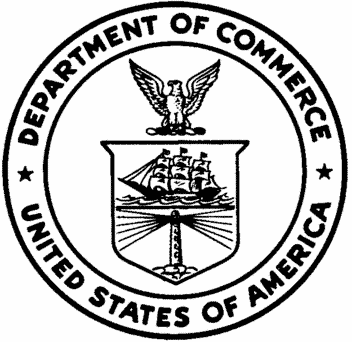
\includegraphics[alt={},width=2cm]{support_files/us_doc_logo.png}\newline % empty curly brackets without alt text is suitable for this logo because it's purely decorative/an "artifact"
  U.S. Department of Commerce\newline
  National Oceanic and Atmospheric Administration\newline
  National Marine Fisheries Service\newline
  Northwest Fisheries Science Center\newline

  \end{minipage}
  \restoregeometry
  \end{titlepage}


\newpage{}

Please cite this publication as:

Wetzel, C.R., and C. Rosemond. 2026. Summary of available Northwest
Fishery Science Center survey data to support assessments of U.S. West
Coast groundfish stocks. Pacific Fisheries Management Council, Portland,
Oregon.

\newpage{}

\hypersetup{linkcolor=.}
\setcounter{tocdepth}{3}
\tableofcontents

\newpage{}

\setlength{\parskip}{5mm plus1mm minus1mm}
\pagenumbering{arabic}
\setcounter{page}{1}
\setcounter{section}{0}
\renewcommand{\thefigure}{\arabic{figure}}
\renewcommand{\thetable}{\arabic{table}}
\setcounter{table}{0}
\setcounter{figure}{0}

\section{Introduction}\label{introduction}

This document provides a detailed summary of commonly used data sources
that may be used to support assessments in 2027. A detailed summary of
data available by year and across sources can allow the Pacific Fishery
Management Council (Council) and advisory bodies to understand the
coverage of data across time and the potential viability of a new
assessment or assessment type.

HIGHLIGHT CHANGES TO THIS YEAR'S REPORT

\subsection{Biological Samples}\label{biological-samples}

Data from the Northwest Fisheries Science Center (NWFSC) West Coast
Groundfish Bottom Trawl Survey (WCGBT) and NWFSC Hook-and-Line (HKL)
surveys are summarized.

Data collected by the NWFSC WCGBT survey between 2003-2024 and the NWFSC
HKL survey from 2004-2024 are summarized by species. Lengths, aged fish,
and unread age structures collected are available by year. Additionally,
the number of tows (NWFSC WCGBT survey) or sites (NWFSC HKL survey) that
observed each species by year are also provided.

\subsection{Survey Length
Compositions}\label{survey-length-compositions}

The length data collected by the NWFSC WCGBT survey were expanded using
a generalized area-based stratification. The composition data were
expanded using a design-based approach with strata based on state
latitudes with two depth strata: 55 - 183 m and 183 - 549 m, with an
exception for four species. The four species have considerable biomass
at depths greater than 549 m: sablefish, Dover sole, longspine
thornyhead, and shortspine thornyhead. Thus an additional depth strata
that covered deeper waters, 549 - 1,280 m, for each state area was
added. The expanded length composition data were summarized using either
a 2 or 4 cm bin structure depending upon the range between maximum and
minimum lengths observed within the survey data. Species where the range
between the maximum and minimum lengths observed by the survey were less
than 60 cm, 2 cm data bins were used, while for species where the range
was 60 cm or greater the data bins were set at 4 cm. All length
observations were treated as unsexed fish in this exercise for
simplicity and for ease of observing potential trends in length
observations across time. The generalized stratification and bin
structure selected here provides a simple summary of the data that can
be useful for decision making, but will likely differ from a
species-specific approach that would be selected in a future assessment.
Additionally, the NWFSC WCGBT survey selectivity for each species will
impact the lengths observed and has not been explicitly accounted for in
this analysis.

The length data collected by the NWFSC HKL survey were summarized to
reflect the proportion of observations by species, length bin, and year.
The length composition data were summarized using either a 2 or 4 cm bin
structure depending upon the range between maximum and minimum lengths
observed within the survey data, in the same manner as for the NWFSC
WCGBT survey. Similar to the NWFSC WCGBT survey, the selectivity of the
NWFSC HKL survey for each species will impact the lengths observed and
has not been explicitly accounted for in this analysis.

\subsection{Survey Relative Indices of
Abundance}\label{survey-relative-indices-of-abundance}

Indices of abundance were estimated from the NWFSC WCGBT survey using a
spatiotemporal model (smdTMB) for species well-observed by the survey.
The indices were estimated using a generalized set-up across species
using either a gamma or log-normal distribution, with the dispersion
parameter held constant across years with 200-500 knots used to create
the mesh. The model structure for each species is provided in Section
\ref{wcgbt-index-settings}. Future species-specific indices of abundance
created with sdmTMB would likely select a more tailored approach for
model settings (e.g., knots, distributions) which could result in slight
changes in year-by-year values for the indices of abundance. The indices
of abundance presented here should only be considered illustrative of
potential trends in abundance across time.

Indices of abundance were estimated from the NWFSC HKL survey for
well-observed species using a negative-binomial model that accounted for
year, site, and drop number. Additional covariates that would typically
be explored when developing species-specific indices for use in stock
assessments were not explored in this analysis for simplicity. The
selection of how to model these data for a particular species may vary
from the approach applied here. For example, the recent vermilion and
sunset rockfish assessment modeled the data as two indices (i.e., one
for areas outside of the Cowcod Conservation Areas {[}CCA{]} and one for
sites inside the CCAs). In contrast, the recent assessment of copper
rockfish estimated a single index with observations by areas weighted
(nearshore sites, northern Channel Islands, Southern Channel Islands).

\subsection{Maturity Data Collections}\label{maturity-data-collections}

Maturity samples for a wide range of West Coast groundfish species have
been collected across a range of sources: NWFSC WCGBT survey, NWFSC HKL
survey, Pacific hake survey, at-sea sampling of the Pacific hake
fishery, and port sampling by ODFW and WDFW. Samples have been collected
between 2009 - 2024. The following summary does not include collection
from the 2025 NWFSC WCGBT and HKL surveys. Summaries of the maturity
collections is provided for each species. This data summary only
includes collections led by the NWFSC but other collections could be
available at the SWFSC, CDFW, ODFW, WDFW, or other research groups.
Future data summaries will look to integrate these additional
collections in subsequent versions of this document.

\subsection{Additional Data}\label{additional-data}

Data may be available for consideration in future assessments that are
currently not included in this report. A summary of potential additional
data that could be available are described below:

\begin{itemize}
\item
  PacFIN and RecFIN.
\item
  Emphasize again that this is only survey data.
\end{itemize}

\newpage{}

\section{Groundfish species observed by surveys conducted by the
NWFSC}\label{groundfish-species-observed-by-surveys-conducted-by-the-nwfsc}

\subsection{Arrowtooth flounder}\label{arrowtooth-flounder}

The most recent assessment of arrowtooth flounder was an update
assessment conducted in 2017. Across available data, arrowtooth flounder
have been observed and sampled by the NWFSC WCGBT survey. The NWFSC
WCGBTS survey has an average of 215 positive tows per year. Across the
coast a total of 254 maturity samples have been collected with 96 read
maturities.

\begingroup\fontsize{10}{12}\selectfont
\begingroup\fontsize{10}{12}\selectfont

\begin{longtable}[t]{>{\raggedleft\arraybackslash}p{2cm}>{\raggedleft\arraybackslash}p{3.5cm}>{\raggedleft\arraybackslash}p{2cm}>{\raggedleft\arraybackslash}p{2cm}>{\raggedleft\arraybackslash}p{2cm}}
\caption{\label{tab:unnamed-chunk-3}Total number of available lengths, read ages, and unread age structures by data source and
state between for arrowtooth flounder.}\\
\toprule
State & Source & Lengths & Ages & Age Structures\\
\midrule
\endfirsthead
\caption[]{Total number of available lengths, read ages, and unread age structures by data source and
state between for arrowtooth flounder. (\textit{continued)}}\\
\toprule
State & Source & Lengths & Ages & Age Structures\\
\midrule
\endhead

\endfoot
\bottomrule
\endlastfoot
CA & NWFSC WCGBTS & 9,814 & 802 & 2,772\\
OR & NWFSC WCGBTS & 29,433 & 2,245 & 7,046\\
WA & NWFSC WCGBTS & 19,722 & 1,281 & 3,896\\*
\end{longtable}
\endgroup{}
\endgroup{}

\begin{figure}[H]

{\centering \pandocbounded{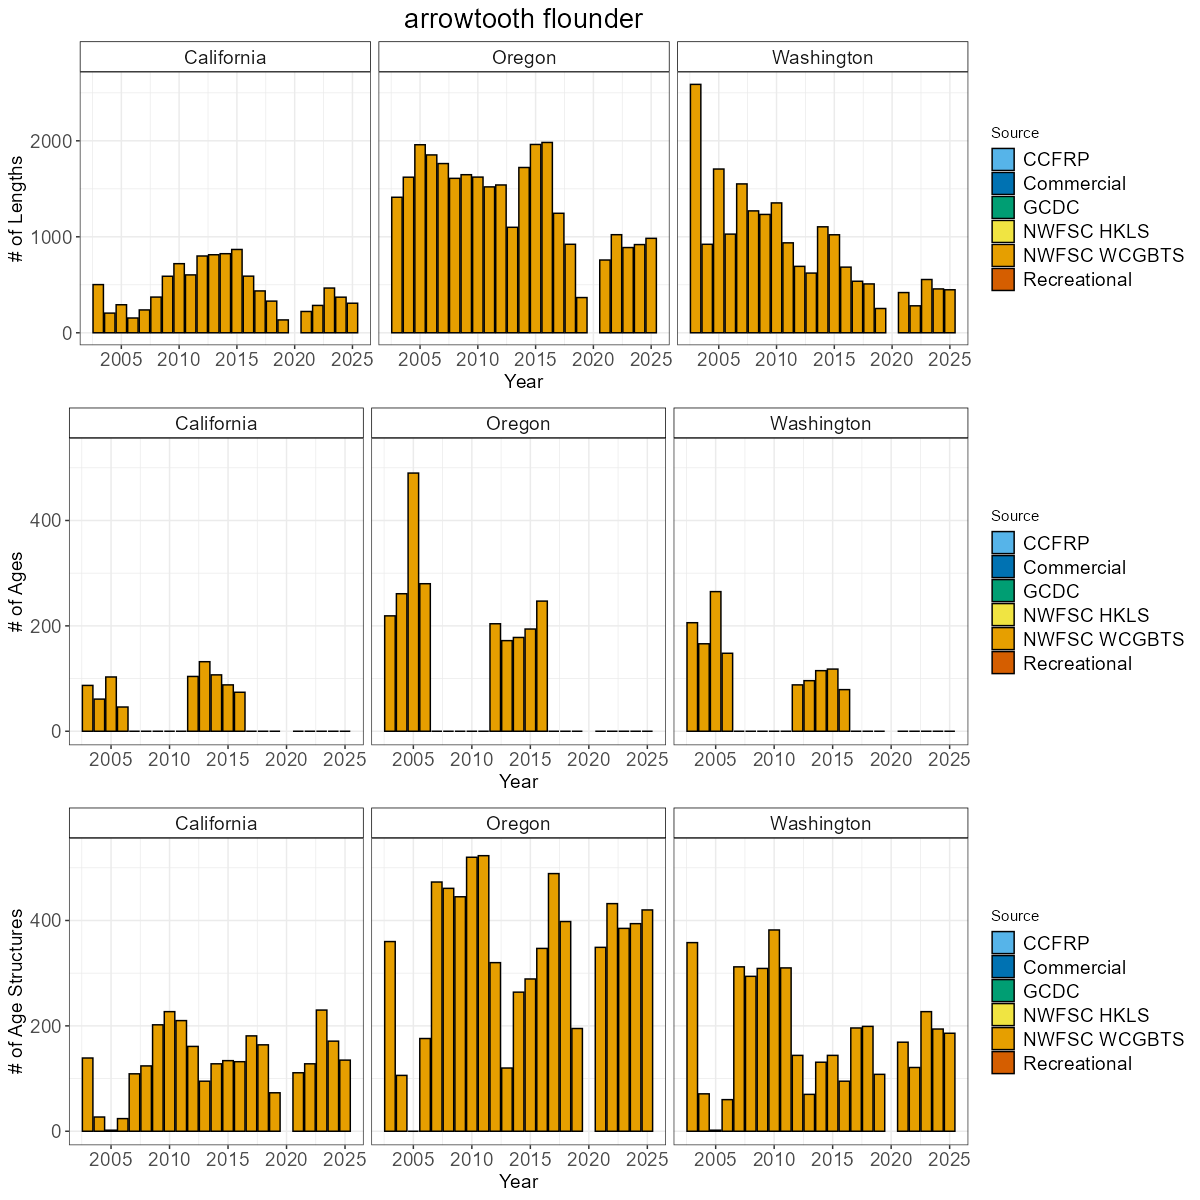
\includegraphics[keepaspectratio]{../plots/state_comparisons/arrowtooth_flounder_state_compositions.png}}

}

\caption{Total number of available lengths, read ages, and unread age
structures by data source by year. Note the y-axis is unique for the
number of lengths plot row compared to the number of age and age
structure plot rows.}

\end{figure}%

\newpage{}

\newpage{}

\subsection{Aurora rockfish}\label{aurora-rockfish}

The most recent assessment of aurora rockfish was a benchmark assessment
conducted in 2013. Across available data, aurora rockfish have been
observed and sampled by the NWFSC WCGBT survey. The NWFSC WCGBTS survey
has an average of 80 positive tows per year. Across the coast a total of
617 maturity samples have been collected with 567 read maturities.

\begingroup\fontsize{10}{12}\selectfont
\begingroup\fontsize{10}{12}\selectfont

\begin{longtable}[t]{>{\raggedleft\arraybackslash}p{2cm}>{\raggedleft\arraybackslash}p{3.5cm}>{\raggedleft\arraybackslash}p{2cm}>{\raggedleft\arraybackslash}p{2cm}>{\raggedleft\arraybackslash}p{2cm}}
\caption{\label{tab:unnamed-chunk-8}Total number of available lengths, read ages, and unread age structures by data source and
state between for aurora rockfish.}\\
\toprule
State & Source & Lengths & Ages & Age Structures\\
\midrule
\endfirsthead
\caption[]{Total number of available lengths, read ages, and unread age structures by data source and
state between for aurora rockfish. (\textit{continued)}}\\
\toprule
State & Source & Lengths & Ages & Age Structures\\
\midrule
\endhead

\endfoot
\bottomrule
\endlastfoot
CA & NWFSC WCGBTS & 26,219 & 2,269 & 7,988\\
OR & NWFSC WCGBTS & 5,453 & 784 & 2,843\\
WA & NWFSC WCGBTS & 384 & 37 & 258\\*
\end{longtable}
\endgroup{}
\endgroup{}

\begin{figure}[H]

{\centering \pandocbounded{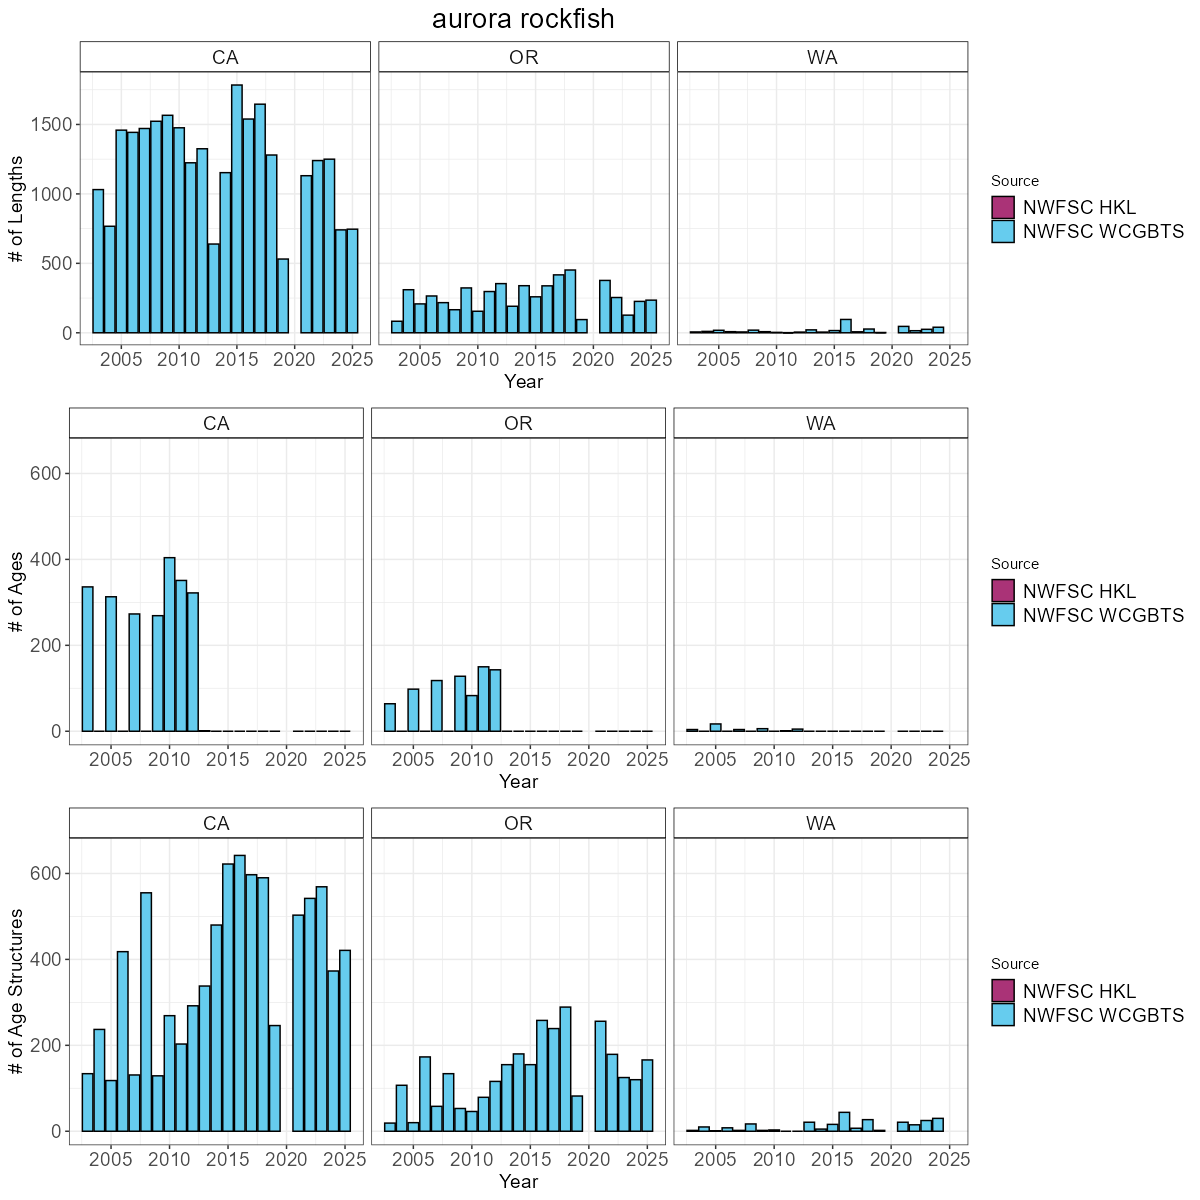
\includegraphics[keepaspectratio]{../plots/state_comparisons/aurora_rockfish_state_compositions.png}}

}

\caption{Total number of available lengths, read ages, and unread age
structures by data source by year. Note the y-axis is unique for the
number of lengths plot row compared to the number of age and age
structure plot rows.}

\end{figure}%

\newpage{}

\subsection{Bank rockfish}\label{bank-rockfish}

To date, no assessment or analysis has been conducted on bank rockfish.
Across available data, bank rockfish have been observed and sampled by
both the NWFSC WCGBT and HKL surveys. The NWFSC HKL survey has an
average of 27 positive tows per year. The NWFSC WCGBTS survey has an
average of 12 positive tows per year. Across the coast a total of 733
maturity samples have been collected with 85 read maturities.

\begingroup\fontsize{10}{12}\selectfont
\begingroup\fontsize{10}{12}\selectfont

\begin{longtable}[t]{>{\raggedleft\arraybackslash}p{2cm}>{\raggedleft\arraybackslash}p{3.5cm}>{\raggedleft\arraybackslash}p{2cm}>{\raggedleft\arraybackslash}p{2cm}>{\raggedleft\arraybackslash}p{2cm}}
\caption{\label{tab:unnamed-chunk-13}Total number of available lengths, read ages, and unread age structures by data source and
state between for bank rockfish.}\\
\toprule
State & Source & Lengths & Ages & Age Structures\\
\midrule
\endfirsthead
\caption[]{Total number of available lengths, read ages, and unread age structures by data source and
state between for bank rockfish. (\textit{continued)}}\\
\toprule
State & Source & Lengths & Ages & Age Structures\\
\midrule
\endhead

\endfoot
\bottomrule
\endlastfoot
CA & NWFSC HKL & 3,666 & 0 & 3,651\\
CA & NWFSC WCGBTS & 2,097 & 0 & 1,455\\
OR & NWFSC WCGBTS & 142 & 0 & 55\\
WA & NWFSC WCGBTS & 4 & 0 & 4\\*
\end{longtable}
\endgroup{}
\endgroup{}

\begin{figure}[H]

{\centering \pandocbounded{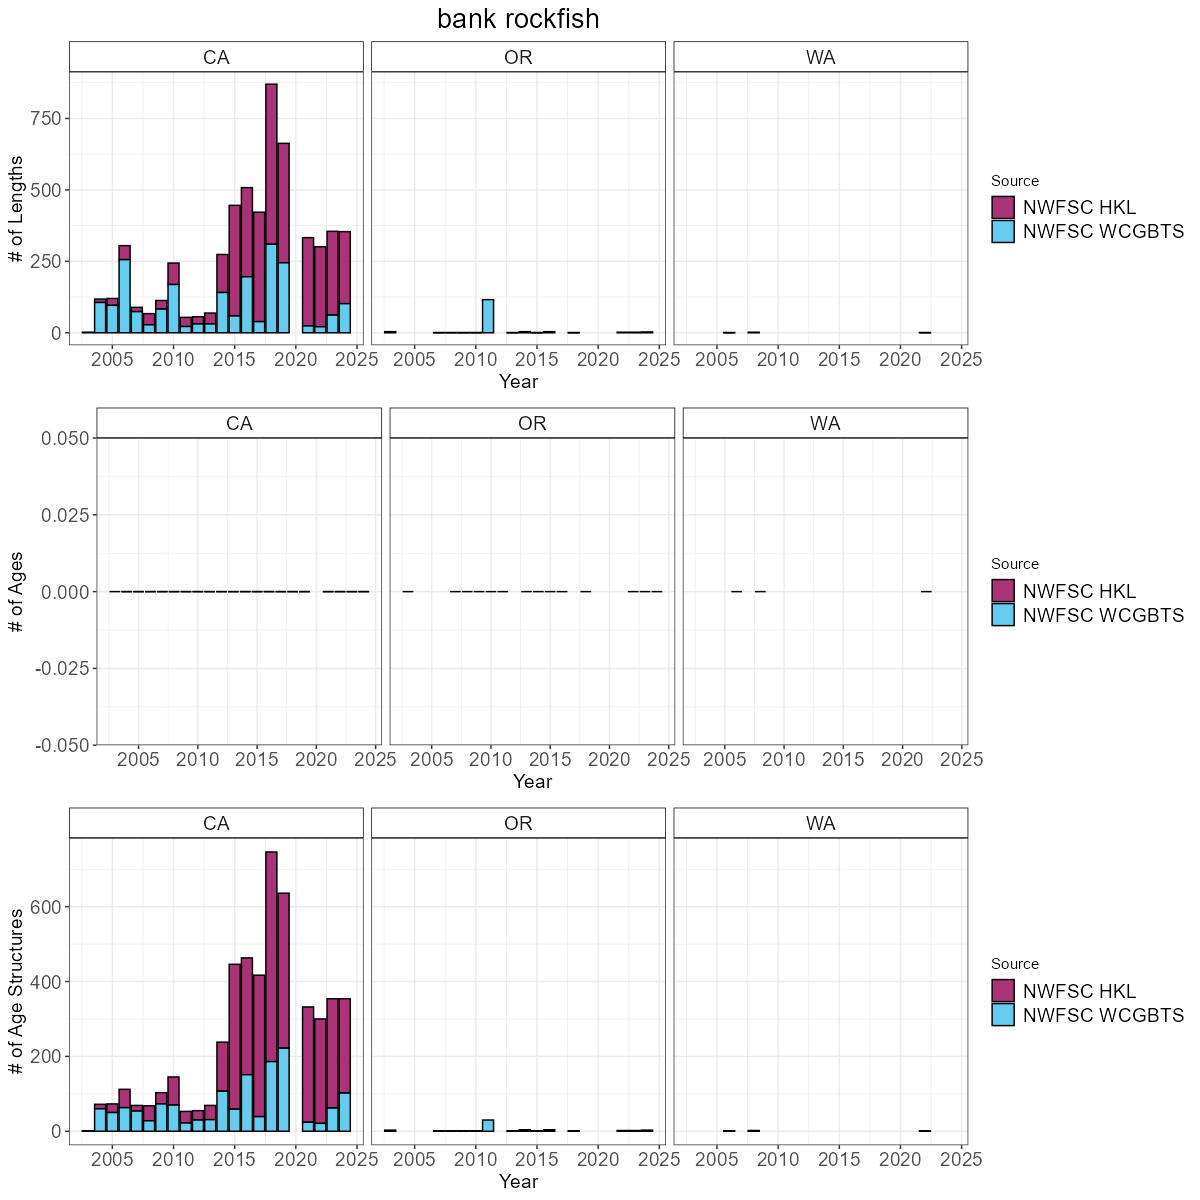
\includegraphics[keepaspectratio]{../plots/state_comparisons/bank_rockfish_state_compositions.png}}

}

\caption{Total number of available lengths, read ages, and unread age
structures by data source by year. Note the y-axis is unique for the
number of lengths plot row compared to the number of age and age
structure plot rows.}

\end{figure}%

\newpage{}

\subsection{Big skate}\label{big-skate}

The most recent assessment of big skate was a benchmark assessment
conducted in 2019. Across available data, big skate have been observed
and sampled by the NWFSC WCGBT survey. The NWFSC WCGBTS survey has an
average of 92 positive tows per year. Across the coast a total of 180
maturity samples have been collected with 180 read maturities.

\begingroup\fontsize{10}{12}\selectfont
\begingroup\fontsize{10}{12}\selectfont

\begin{longtable}[t]{>{\raggedleft\arraybackslash}p{2cm}>{\raggedleft\arraybackslash}p{3.5cm}>{\raggedleft\arraybackslash}p{2cm}>{\raggedleft\arraybackslash}p{2cm}>{\raggedleft\arraybackslash}p{2cm}}
\caption{\label{tab:unnamed-chunk-18}Total number of available lengths, read ages, and unread age structures by data source and
state between for big skate.}\\
\toprule
State & Source & Lengths & Ages & Age Structures\\
\midrule
\endfirsthead
\caption[]{Total number of available lengths, read ages, and unread age structures by data source and
state between for big skate. (\textit{continued)}}\\
\toprule
State & Source & Lengths & Ages & Age Structures\\
\midrule
\endhead

\endfoot
\bottomrule
\endlastfoot
CA & NWFSC WCGBTS & 2,263 & 351 & 132\\
OR & NWFSC WCGBTS & 2,651 & 422 & 331\\
WA & NWFSC WCGBTS & 1,987 & 261 & 235\\*
\end{longtable}
\endgroup{}
\endgroup{}

\begin{figure}[H]

{\centering \pandocbounded{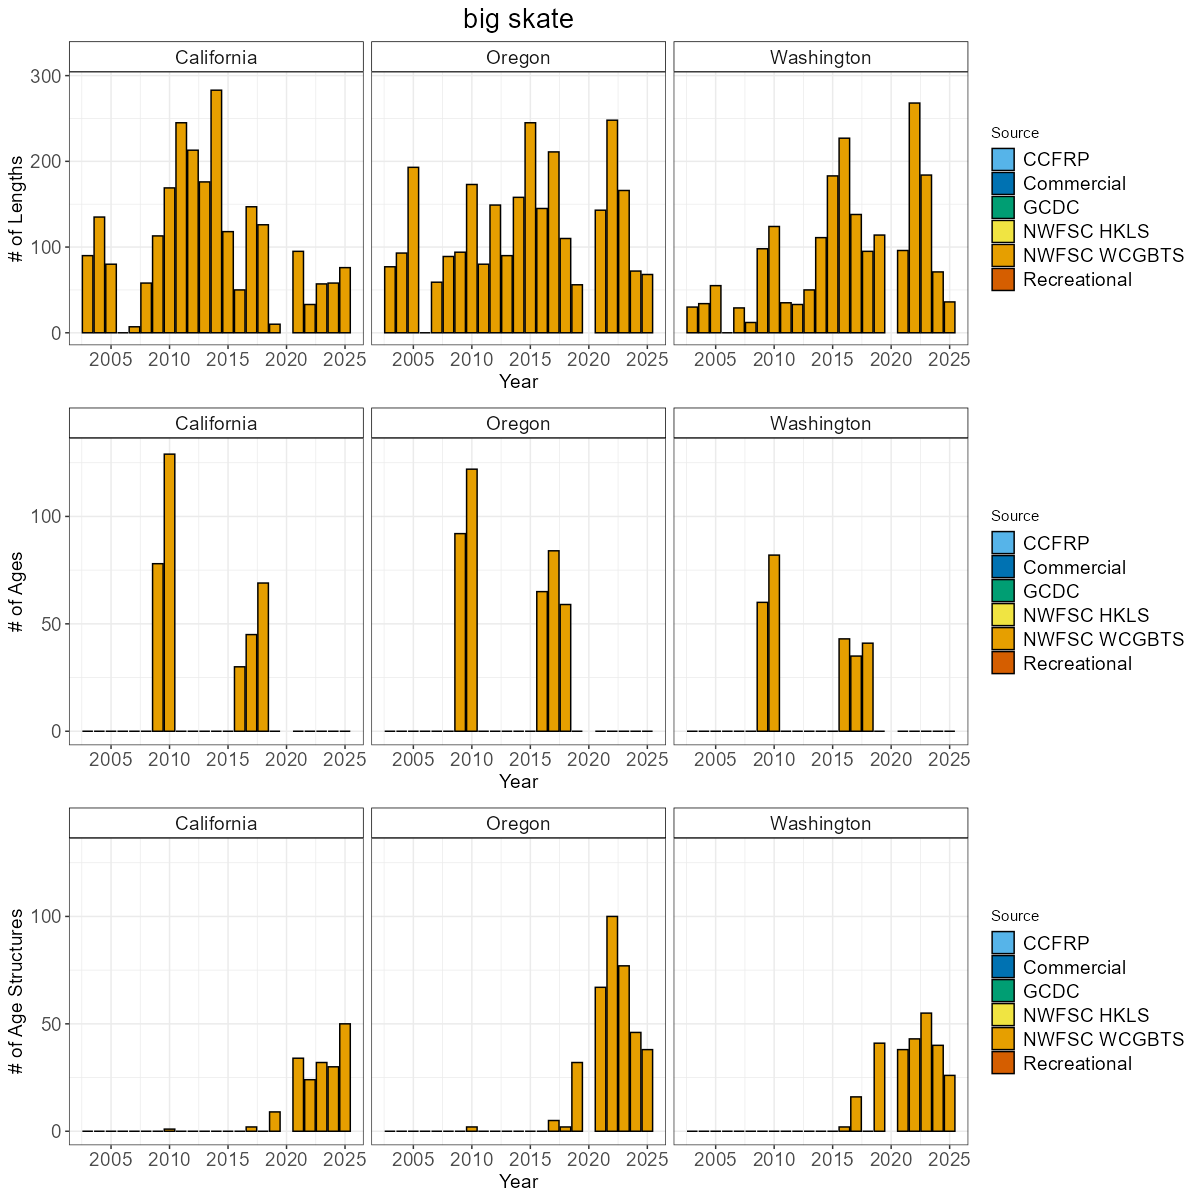
\includegraphics[keepaspectratio]{../plots/state_comparisons/big_skate_state_compositions.png}}

}

\caption{Total number of available lengths, read ages, and unread age
structures by data source by year. Note the y-axis is unique for the
number of lengths plot row compared to the number of age and age
structure plot rows.}

\end{figure}%

\newpage{}

\subsection{Blackgill rockfish}\label{blackgill-rockfish}

The most recent assessment of blackgill rockfish was an update
assessment conducted in 2017. Across available data, blackgill rockfish
have been observed and sampled by the NWFSC WCGBT survey. The NWFSC
WCGBTS survey has an average of 34 positive tows per year. Across the
coast a total of 126 maturity samples have been collected with 126 read
maturities.

\begingroup\fontsize{10}{12}\selectfont
\begingroup\fontsize{10}{12}\selectfont

\begin{longtable}[t]{>{\raggedleft\arraybackslash}p{2cm}>{\raggedleft\arraybackslash}p{3.5cm}>{\raggedleft\arraybackslash}p{2cm}>{\raggedleft\arraybackslash}p{2cm}>{\raggedleft\arraybackslash}p{2cm}}
\caption{\label{tab:unnamed-chunk-24}Total number of available lengths, read ages, and unread age structures by data source and
state between for blackgill rockfish.}\\
\toprule
State & Source & Lengths & Ages & Age Structures\\
\midrule
\endfirsthead
\caption[]{Total number of available lengths, read ages, and unread age structures by data source and
state between for blackgill rockfish. (\textit{continued)}}\\
\toprule
State & Source & Lengths & Ages & Age Structures\\
\midrule
\endhead

\endfoot
\bottomrule
\endlastfoot
CA & NWFSC HKL & 7 & 0 & 7\\
CA & NWFSC WCGBTS & 10,484 & 1,937 & 5,586\\
OR & NWFSC WCGBTS & 286 & 11 & 254\\
WA & NWFSC WCGBTS & 7 & 0 & 7\\*
\end{longtable}
\endgroup{}
\endgroup{}

\begin{figure}[H]

{\centering \pandocbounded{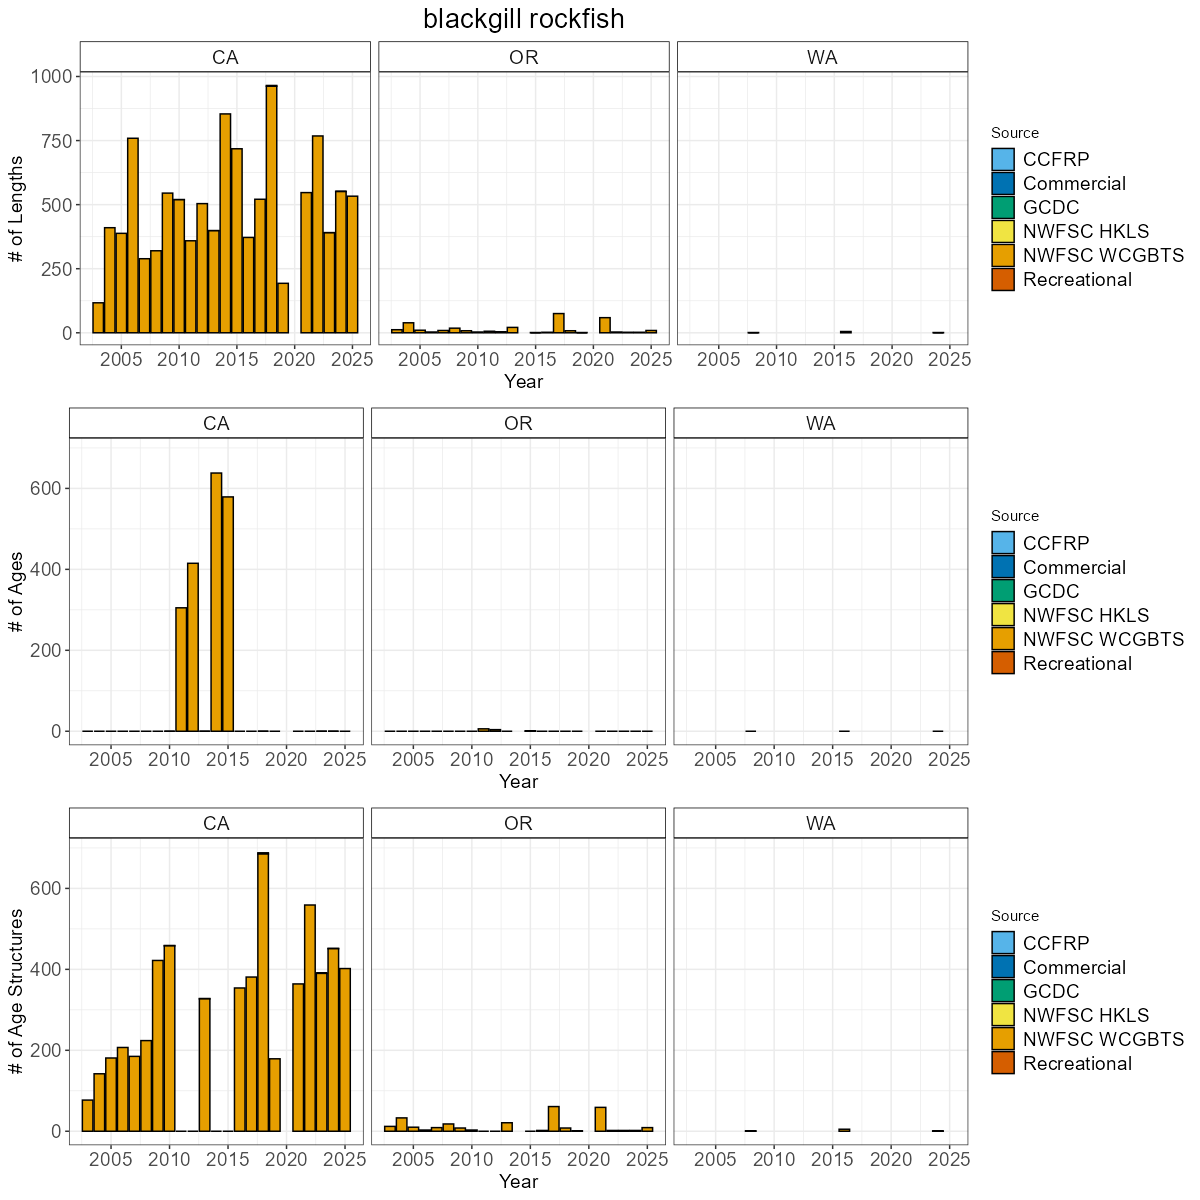
\includegraphics[keepaspectratio]{../plots/state_comparisons/blackgill_rockfish_state_compositions.png}}

}

\caption{Total number of available lengths, read ages, and unread age
structures by data source by year. Note the y-axis is unique for the
number of lengths plot row compared to the number of age and age
structure plot rows.}

\end{figure}%

\newpage{}

\subsection{Bocaccio}\label{bocaccio}

The most recent assessment of bocaccio was an update assessment
conducted in 2017. Across available data, bocaccio have been observed
and sampled by both the NWFSC WCGBT and HKL surveys. The NWFSC HKL
survey has an average of 112 positive tows per year. The NWFSC WCGBTS
survey has an average of 49 positive tows per year. Across the coast a
total of 837 maturity samples have been collected with 737 read
maturities.

\begingroup\fontsize{10}{12}\selectfont
\begingroup\fontsize{10}{12}\selectfont

\begin{longtable}[t]{>{\raggedleft\arraybackslash}p{2cm}>{\raggedleft\arraybackslash}p{3.5cm}>{\raggedleft\arraybackslash}p{2cm}>{\raggedleft\arraybackslash}p{2cm}>{\raggedleft\arraybackslash}p{2cm}}
\caption{\label{tab:unnamed-chunk-29}Total number of available lengths, read ages, and unread age structures by data source and
state between for bocaccio.}\\
\toprule
State & Source & Lengths & Ages & Age Structures\\
\midrule
\endfirsthead
\caption[]{Total number of available lengths, read ages, and unread age structures by data source and
state between for bocaccio. (\textit{continued)}}\\
\toprule
State & Source & Lengths & Ages & Age Structures\\
\midrule
\endhead

\endfoot
\bottomrule
\endlastfoot
CA & NWFSC HKL & 21,333 & 0 & 13,842\\
CA & NWFSC WCGBTS & 10,436 & 2,759 & 3,969\\
OR & NWFSC WCGBTS & 294 & 20 & 180\\
WA & NWFSC WCGBTS & 477 & 74 & 333\\*
\end{longtable}
\endgroup{}
\endgroup{}

\begin{figure}[H]

{\centering \pandocbounded{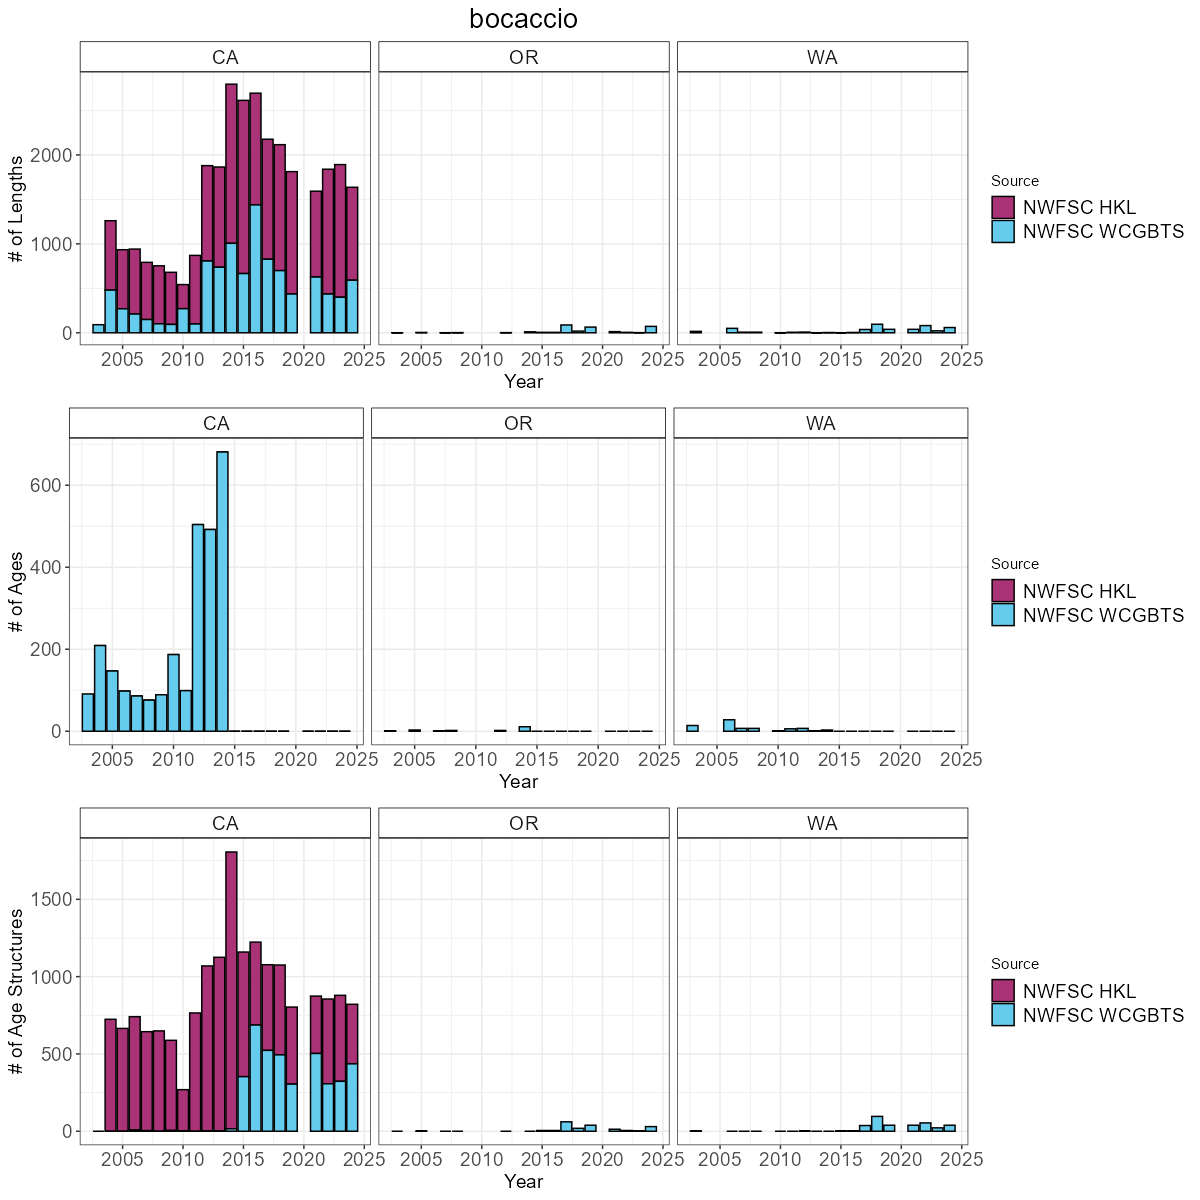
\includegraphics[keepaspectratio]{../plots/state_comparisons/bocaccio_state_compositions.png}}

}

\caption{Total number of available lengths, read ages, and unread age
structures by data source by year. Note the y-axis is unique for the
number of lengths plot row compared to the number of age and age
structure plot rows.}

\end{figure}%

\newpage{}

\subsection{California scorpionfish}\label{california-scorpionfish}

The most recent assessment of California scorpionfish was a benchmark
assessment conducted in 2017. Across available data, California
scorpionfish have been observed and sampled by both the NWFSC WCGBT and
HKL surveys. The NWFSC WCGBTS survey has an average of 12 positive tows
per year. Across the coast a total of 0 maturity samples have been
collected with 0 read maturities.

\begingroup\fontsize{10}{12}\selectfont
\begingroup\fontsize{10}{12}\selectfont

\begin{longtable}[t]{>{\raggedleft\arraybackslash}p{2cm}>{\raggedleft\arraybackslash}p{3.5cm}>{\raggedleft\arraybackslash}p{2cm}>{\raggedleft\arraybackslash}p{2cm}>{\raggedleft\arraybackslash}p{2cm}}
\caption{\label{tab:unnamed-chunk-35}Total number of available lengths, read ages, and unread age structures by data source and
state between for California scorpionfish.}\\
\toprule
State & Source & Lengths & Ages & Age Structures\\
\midrule
\endfirsthead
\caption[]{Total number of available lengths, read ages, and unread age structures by data source and
state between for California scorpionfish. (\textit{continued)}}\\
\toprule
State & Source & Lengths & Ages & Age Structures\\
\midrule
\endhead

\endfoot
\bottomrule
\endlastfoot
CA & NWFSC HKL & 41 & 0 & 23\\
CA & NWFSC WCGBTS & 4,203 & 911 & 1,044\\*
\end{longtable}
\endgroup{}
\endgroup{}

\begin{figure}[H]

{\centering \pandocbounded{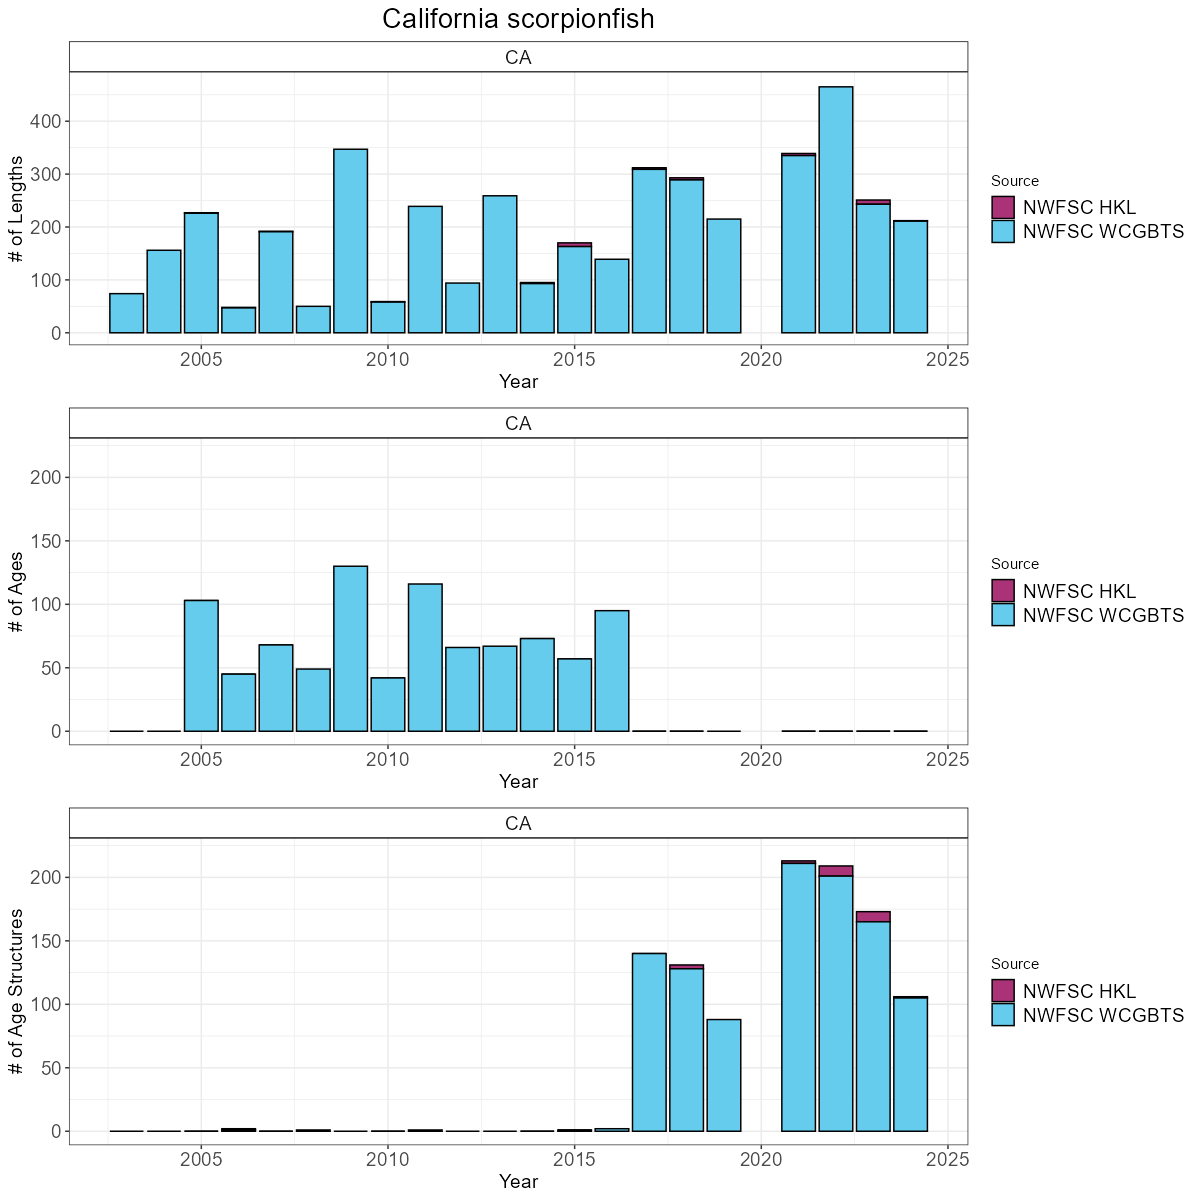
\includegraphics[keepaspectratio]{../plots/state_comparisons/california_scorpionfish_state_compositions.png}}

}

\caption{Total number of available lengths, read ages, and unread age
structures by data source by year. Note the y-axis is unique for the
number of lengths plot row compared to the number of age and age
structure plot rows.}

\end{figure}%

\newpage{}

\subsection{Canary rockfish}\label{canary-rockfish}

The most recent assessment of canary rockfish was a benchmark assessment
conducted in 2023. Across available data, canary rockfish have been
observed and sampled by both the NWFSC WCGBT and HKL surveys. The NWFSC
HKL survey has an average of 7 positive tows per year. The NWFSC WCGBTS
survey has an average of 51 positive tows per year. Across the coast a
total of 1480 maturity samples have been collected with 1184 read
maturities. ODFW scientists are planning a research cruise to Cobb Sea
Mount in the summer of 2026 to sample age and sex distributions of
rockfish species.

\begingroup\fontsize{10}{12}\selectfont
\begingroup\fontsize{10}{12}\selectfont

\begin{longtable}[t]{>{\raggedleft\arraybackslash}p{2cm}>{\raggedleft\arraybackslash}p{3.5cm}>{\raggedleft\arraybackslash}p{2cm}>{\raggedleft\arraybackslash}p{2cm}>{\raggedleft\arraybackslash}p{2cm}}
\caption{\label{tab:unnamed-chunk-40}Total number of available lengths, read ages, and unread age structures by data source and
state between for canary rockfish.}\\
\toprule
State & Source & Lengths & Ages & Age Structures\\
\midrule
\endfirsthead
\caption[]{Total number of available lengths, read ages, and unread age structures by data source and
state between for canary rockfish. (\textit{continued)}}\\
\toprule
State & Source & Lengths & Ages & Age Structures\\
\midrule
\endhead

\endfoot
\bottomrule
\endlastfoot
CA & NWFSC HKL & 553 & 511 & 38\\
CA & NWFSC WCGBTS & 3,397 & 1,854 & 190\\
OR & NWFSC WCGBTS & 4,893 & 3,178 & 138\\
WA & NWFSC WCGBTS & 6,382 & 3,430 & 377\\*
\end{longtable}
\endgroup{}
\endgroup{}

\begin{figure}[H]

{\centering \pandocbounded{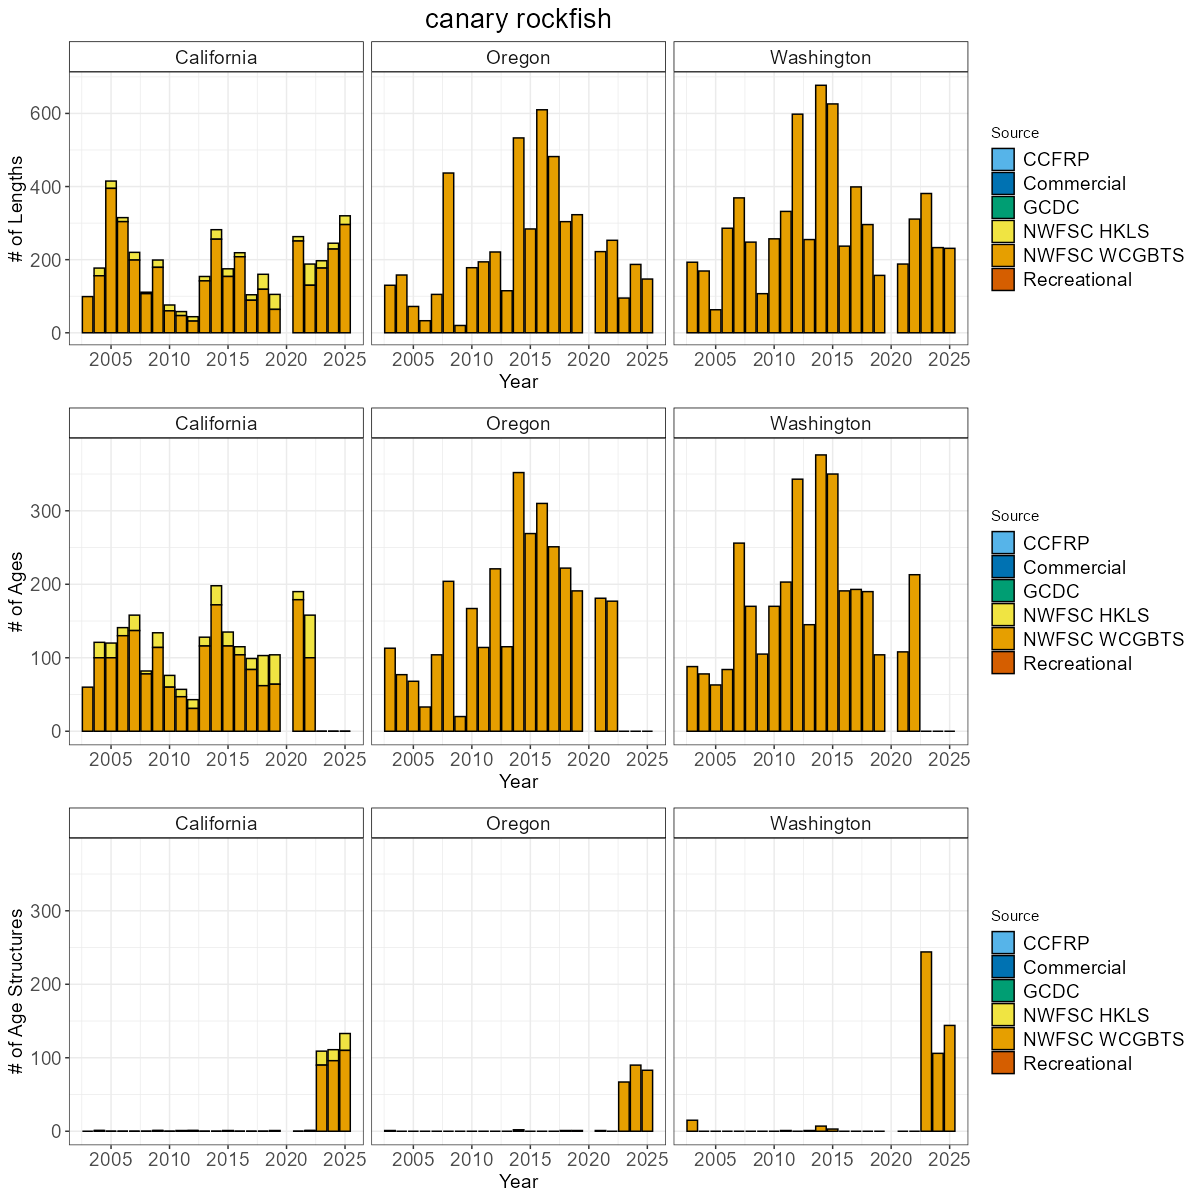
\includegraphics[keepaspectratio]{../plots/state_comparisons/canary_rockfish_state_compositions.png}}

}

\caption{Total number of available lengths, read ages, and unread age
structures by data source by year. Note the y-axis is unique for the
number of lengths plot row compared to the number of age and age
structure plot rows.}

\end{figure}%

\newpage{}

\subsection{Chilipepper}\label{chilipepper}

The most recent assessment of chilipepper was a benchmark assessment
conducted in 2025. Across available data, chilipepper have been observed
and sampled by both the NWFSC WCGBT and HKL surveys. The NWFSC HKL
survey has an average of 25 positive tows per year. The NWFSC WCGBTS
survey has an average of 88 positive tows per year. Across the coast a
total of 157 maturity samples have been collected with 157 read
maturities.

\begingroup\fontsize{10}{12}\selectfont
\begingroup\fontsize{10}{12}\selectfont

\begin{longtable}[t]{>{\raggedleft\arraybackslash}p{2cm}>{\raggedleft\arraybackslash}p{3.5cm}>{\raggedleft\arraybackslash}p{2cm}>{\raggedleft\arraybackslash}p{2cm}>{\raggedleft\arraybackslash}p{2cm}}
\caption{\label{tab:unnamed-chunk-45}Total number of available lengths, read ages, and unread age structures by data source and
state between for chilipepper.}\\
\toprule
State & Source & Lengths & Ages & Age Structures\\
\midrule
\endfirsthead
\caption[]{Total number of available lengths, read ages, and unread age structures by data source and
state between for chilipepper. (\textit{continued)}}\\
\toprule
State & Source & Lengths & Ages & Age Structures\\
\midrule
\endhead

\endfoot
\bottomrule
\endlastfoot
CA & NWFSC HKL & 2,881 & 249 & 2,449\\
CA & NWFSC WCGBTS & 33,744 & 12,386 & 728\\
OR & NWFSC WCGBTS & 2,182 & 904 & 57\\
WA & NWFSC WCGBTS & 27 & 27 & 0\\*
\end{longtable}
\endgroup{}
\endgroup{}

\begin{figure}[H]

{\centering \pandocbounded{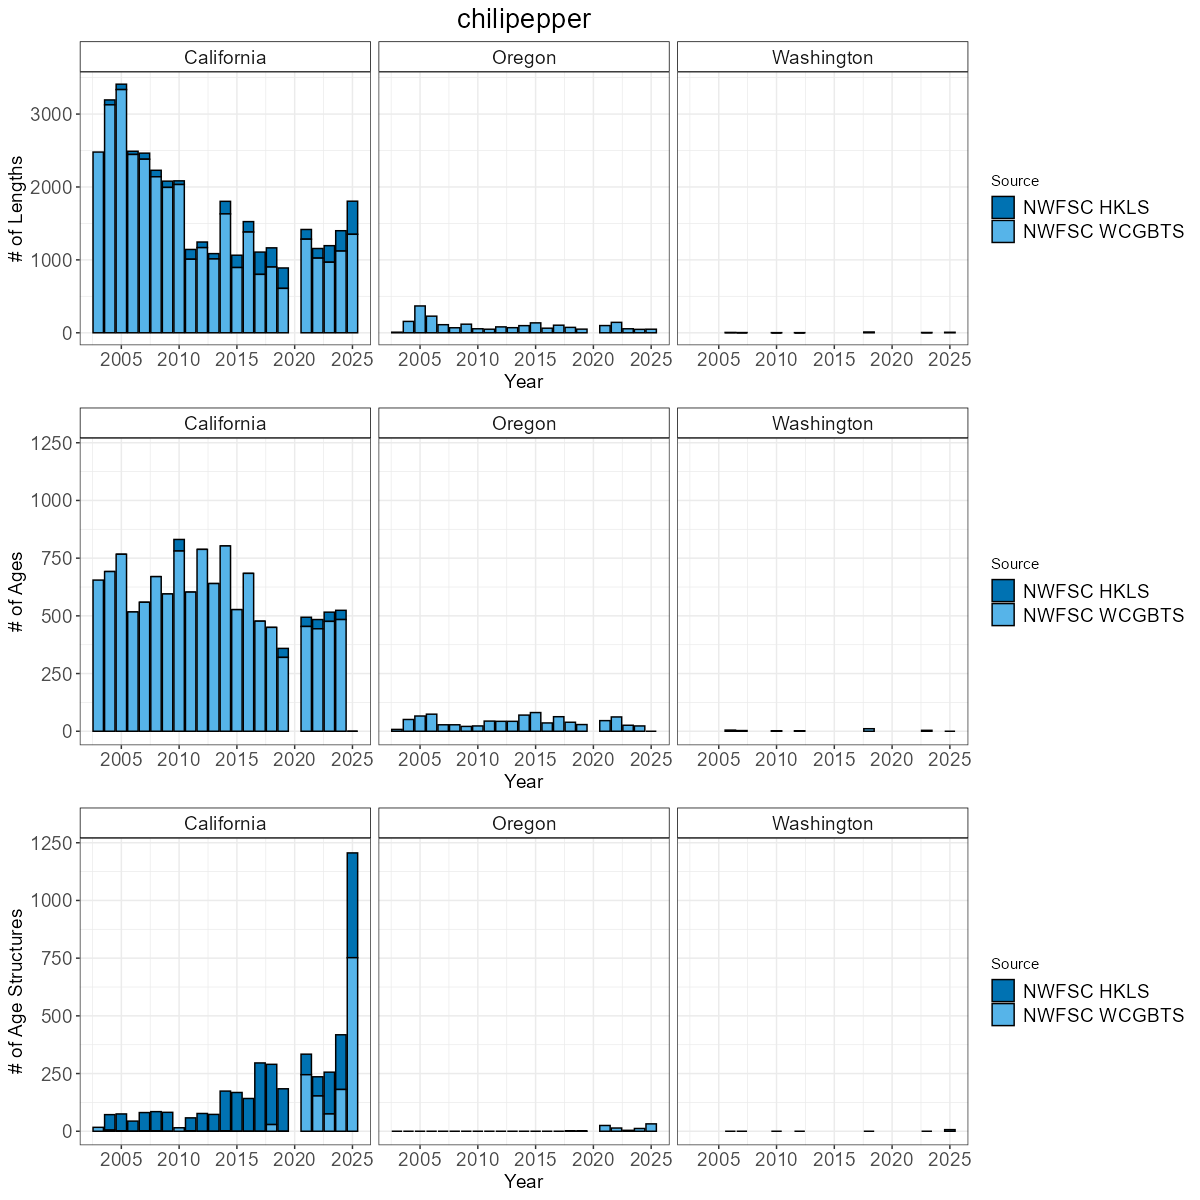
\includegraphics[keepaspectratio]{../plots/state_comparisons/chilipepper_state_compositions.png}}

}

\caption{Total number of available lengths, read ages, and unread age
structures by data source by year. Note the y-axis is unique for the
number of lengths plot row compared to the number of age and age
structure plot rows.}

\end{figure}%

\newpage{}

\subsection{Darkblotched rockfish}\label{darkblotched-rockfish}

The most recent assessment of darkblotched rockfish was an update
assessment conducted in 2017. Across available data, darkblotched
rockfish have been observed and sampled by the NWFSC WCGBT survey. The
NWFSC WCGBTS survey has an average of 107 positive tows per year. Across
the coast a total of 958 maturity samples have been collected with 927
read maturities.

\begingroup\fontsize{10}{12}\selectfont
\begingroup\fontsize{10}{12}\selectfont

\begin{longtable}[t]{>{\raggedleft\arraybackslash}p{2cm}>{\raggedleft\arraybackslash}p{3.5cm}>{\raggedleft\arraybackslash}p{2cm}>{\raggedleft\arraybackslash}p{2cm}>{\raggedleft\arraybackslash}p{2cm}}
\caption{\label{tab:unnamed-chunk-51}Total number of available lengths, read ages, and unread age structures by data source and
state between for darkblotched rockfish.}\\
\toprule
State & Source & Lengths & Ages & Age Structures\\
\midrule
\endfirsthead
\caption[]{Total number of available lengths, read ages, and unread age structures by data source and
state between for darkblotched rockfish. (\textit{continued)}}\\
\toprule
State & Source & Lengths & Ages & Age Structures\\
\midrule
\endhead

\endfoot
\bottomrule
\endlastfoot
CA & NWFSC WCGBTS & 7,634 & 2,561 & 925\\
OR & NWFSC WCGBTS & 22,610 & 6,636 & 2,941\\
WA & NWFSC WCGBTS & 8,474 & 2,523 & 789\\*
\end{longtable}
\endgroup{}
\endgroup{}

\begin{figure}[H]

{\centering \pandocbounded{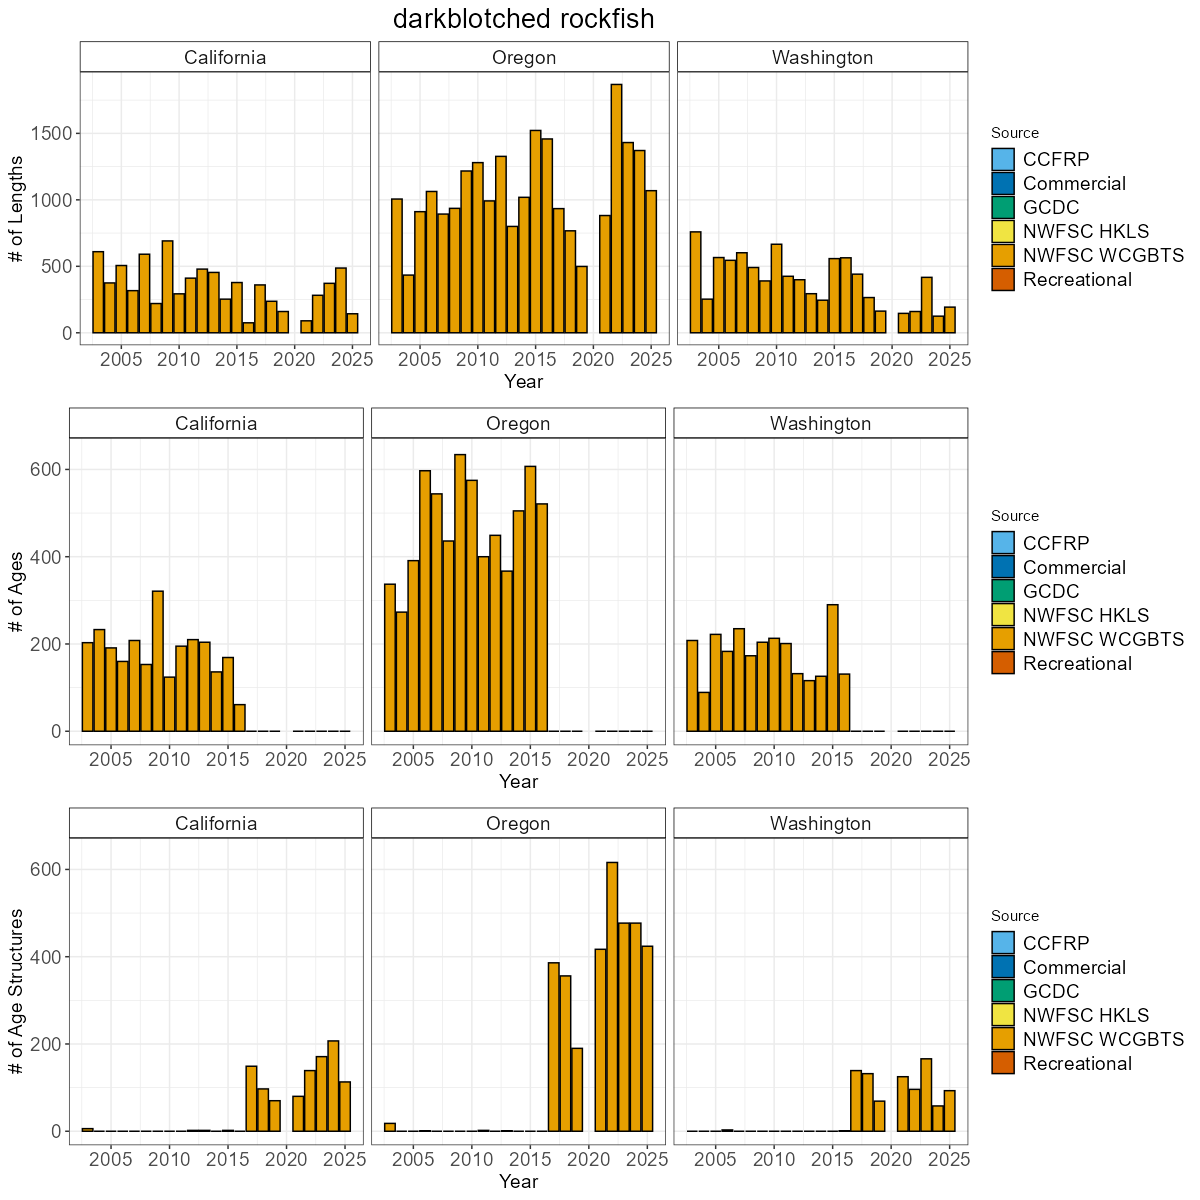
\includegraphics[keepaspectratio]{../plots/state_comparisons/darkblotched_rockfish_state_compositions.png}}

}

\caption{Total number of available lengths, read ages, and unread age
structures by data source by year. Note the y-axis is unique for the
number of lengths plot row compared to the number of age and age
structure plot rows.}

\end{figure}%

\newpage{}

\subsection{Dover sole}\label{dover-sole}

The most recent assessment of Dover sole was a benchmark assessment
conducted in 2021. Across available data, Dover sole have been observed
and sampled by the NWFSC WCGBT survey. The NWFSC WCGBTS survey has an
average of 508 positive tows per year. Across the coast a total of 820
maturity samples have been collected with 635 read maturities.

\begingroup\fontsize{10}{12}\selectfont
\begingroup\fontsize{10}{12}\selectfont

\begin{longtable}[t]{>{\raggedleft\arraybackslash}p{2cm}>{\raggedleft\arraybackslash}p{3.5cm}>{\raggedleft\arraybackslash}p{2cm}>{\raggedleft\arraybackslash}p{2cm}>{\raggedleft\arraybackslash}p{2cm}}
\caption{\label{tab:unnamed-chunk-56}Total number of available lengths, read ages, and unread age structures by data source and
state between for Dover sole.}\\
\toprule
State & Source & Lengths & Ages & Age Structures\\
\midrule
\endfirsthead
\caption[]{Total number of available lengths, read ages, and unread age structures by data source and
state between for Dover sole. (\textit{continued)}}\\
\toprule
State & Source & Lengths & Ages & Age Structures\\
\midrule
\endhead

\endfoot
\bottomrule
\endlastfoot
CA & NWFSC WCGBTS & 86,127 & 8,700 & 5,775\\
OR & NWFSC WCGBTS & 69,163 & 5,836 & 4,155\\
WA & NWFSC WCGBTS & 32,188 & 2,581 & 1,982\\*
\end{longtable}
\endgroup{}
\endgroup{}

\begin{figure}[H]

{\centering \pandocbounded{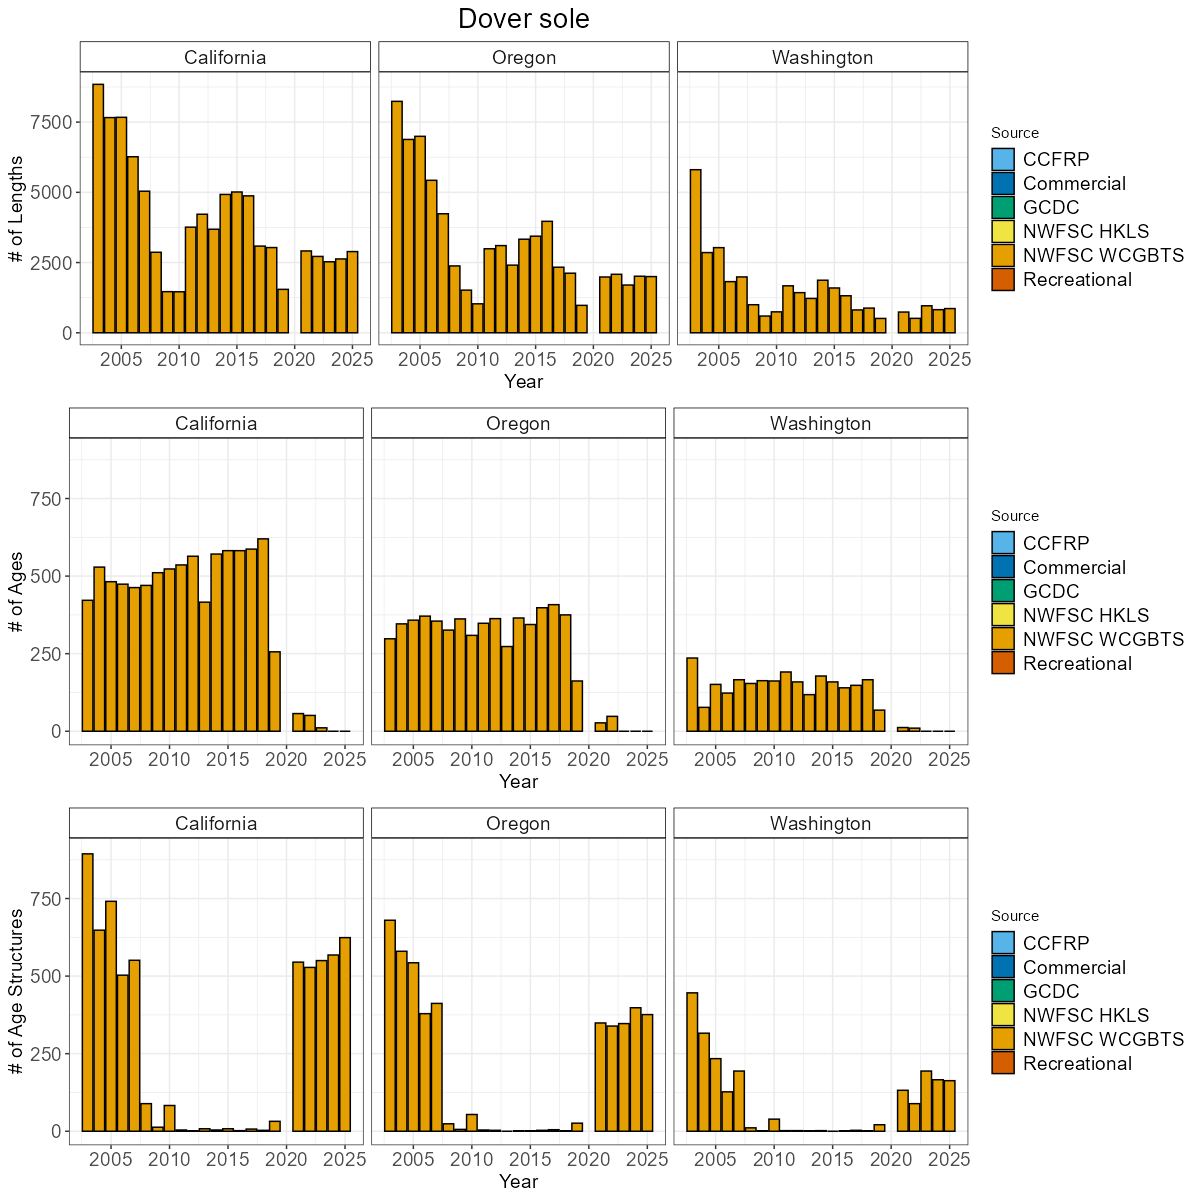
\includegraphics[keepaspectratio]{../plots/state_comparisons/dover_sole_state_compositions.png}}

}

\caption{Total number of available lengths, read ages, and unread age
structures by data source by year. Note the y-axis is unique for the
number of lengths plot row compared to the number of age and age
structure plot rows.}

\end{figure}%

\newpage{}

\subsection{English sole}\label{english-sole}

The most recent assessment of English sole was a data-moderate
assessment conducted in 2013. Across available data, English sole have
been observed and sampled by the NWFSC WCGBT survey. The NWFSC WCGBTS
survey has an average of 253 positive tows per year. Across the coast a
total of 174 maturity samples have been collected with 0 read
maturities.

\begingroup\fontsize{10}{12}\selectfont
\begingroup\fontsize{10}{12}\selectfont

\begin{longtable}[t]{>{\raggedleft\arraybackslash}p{2cm}>{\raggedleft\arraybackslash}p{3.5cm}>{\raggedleft\arraybackslash}p{2cm}>{\raggedleft\arraybackslash}p{2cm}>{\raggedleft\arraybackslash}p{2cm}}
\caption{\label{tab:unnamed-chunk-61}Total number of available lengths, read ages, and unread age structures by data source and
state between for English sole.}\\
\toprule
State & Source & Lengths & Ages & Age Structures\\
\midrule
\endfirsthead
\caption[]{Total number of available lengths, read ages, and unread age structures by data source and
state between for English sole. (\textit{continued)}}\\
\toprule
State & Source & Lengths & Ages & Age Structures\\
\midrule
\endhead

\endfoot
\bottomrule
\endlastfoot
CA & NWFSC WCGBTS & 44,691 & 478 & 8,824\\
OR & NWFSC WCGBTS & 31,096 & 279 & 5,347\\
WA & NWFSC WCGBTS & 13,520 & 141 & 2,882\\*
\end{longtable}
\endgroup{}
\endgroup{}

\begin{figure}[H]

{\centering \pandocbounded{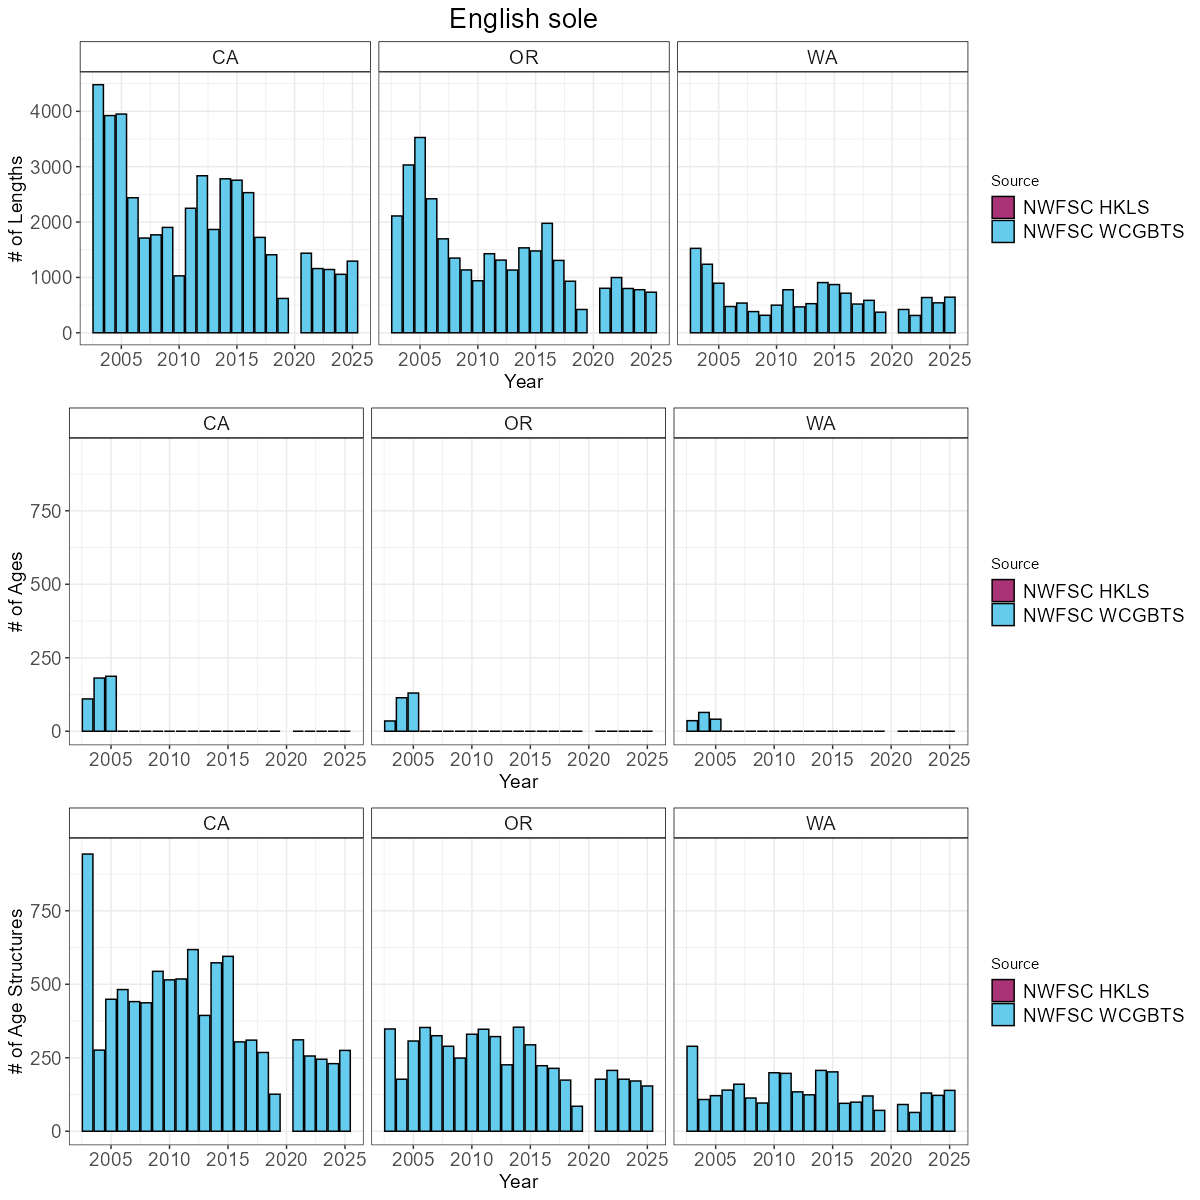
\includegraphics[keepaspectratio]{../plots/state_comparisons/english_sole_state_compositions.png}}

}

\caption{Total number of available lengths, read ages, and unread age
structures by data source by year. Note the y-axis is unique for the
number of lengths plot row compared to the number of age and age
structure plot rows.}

\end{figure}%

\newpage{}

\subsection{Flathead sole}\label{flathead-sole}

To date, no assessment or analysis has been conducted on flathead sole.
Across available data, flathead sole have been observed and sampled by
the NWFSC WCGBT survey. The NWFSC WCGBTS survey has an average of 49
positive tows per year. Across the coast a total of 0 maturity samples
have been collected with 0 read maturities.

\begingroup\fontsize{10}{12}\selectfont
\begingroup\fontsize{10}{12}\selectfont

\begin{longtable}[t]{>{\raggedleft\arraybackslash}p{2cm}>{\raggedleft\arraybackslash}p{3.5cm}>{\raggedleft\arraybackslash}p{2cm}>{\raggedleft\arraybackslash}p{2cm}>{\raggedleft\arraybackslash}p{2cm}}
\caption{\label{tab:unnamed-chunk-66}Total number of available lengths, read ages, and unread age structures by data source and
state between for flathead sole.}\\
\toprule
State & Source & Lengths & Ages & Age Structures\\
\midrule
\endfirsthead
\caption[]{Total number of available lengths, read ages, and unread age structures by data source and
state between for flathead sole. (\textit{continued)}}\\
\toprule
State & Source & Lengths & Ages & Age Structures\\
\midrule
\endhead

\endfoot
\bottomrule
\endlastfoot
CA & NWFSC WCGBTS & 76 & 0 & 38\\
OR & NWFSC WCGBTS & 4,776 & 0 & 2,009\\
WA & NWFSC WCGBTS & 7,168 & 0 & 1,639\\*
\end{longtable}
\endgroup{}
\endgroup{}

\begin{figure}[H]

{\centering \pandocbounded{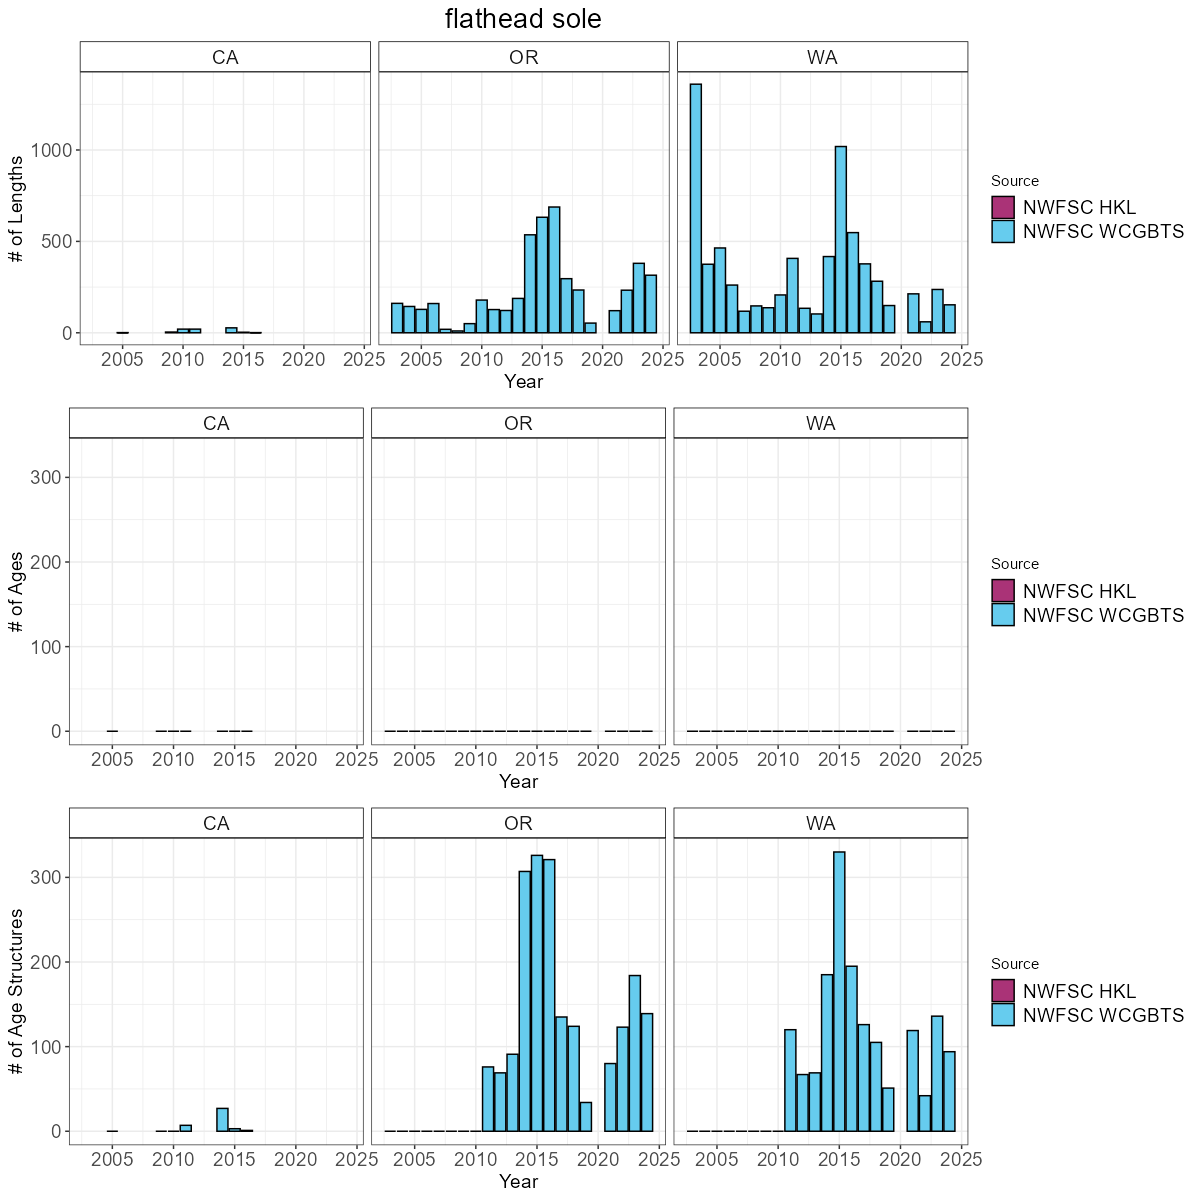
\includegraphics[keepaspectratio]{../plots/state_comparisons/flathead_sole_state_compositions.png}}

}

\caption{Total number of available lengths, read ages, and unread age
structures by data source by year. Note the y-axis is unique for the
number of lengths plot row compared to the number of age and age
structure plot rows.}

\end{figure}%

\newpage{}

\subsection{Greenspotted rockfish}\label{greenspotted-rockfish}

The most recent assessment of greenspotted rockfish was a benchmark
assessment conducted in 2011. Across available data, greenspotted
rockfish have been observed and sampled by both the NWFSC WCGBT and HKL
surveys. The NWFSC HKL survey has an average of 61 positive tows per
year. The NWFSC WCGBTS survey has an average of 33 positive tows per
year. Across the coast a total of 338 maturity samples have been
collected with 175 read maturities.

\begingroup\fontsize{10}{12}\selectfont
\begingroup\fontsize{10}{12}\selectfont

\begin{longtable}[t]{>{\raggedleft\arraybackslash}p{2cm}>{\raggedleft\arraybackslash}p{3.5cm}>{\raggedleft\arraybackslash}p{2cm}>{\raggedleft\arraybackslash}p{2cm}>{\raggedleft\arraybackslash}p{2cm}}
\caption{\label{tab:unnamed-chunk-71}Total number of available lengths, read ages, and unread age structures by data source and
state between for greenspotted rockfish.}\\
\toprule
State & Source & Lengths & Ages & Age Structures\\
\midrule
\endfirsthead
\caption[]{Total number of available lengths, read ages, and unread age structures by data source and
state between for greenspotted rockfish. (\textit{continued)}}\\
\toprule
State & Source & Lengths & Ages & Age Structures\\
\midrule
\endhead

\endfoot
\bottomrule
\endlastfoot
CA & NWFSC HKL & 6,110 & 843 & 5,090\\
CA & NWFSC WCGBTS & 7,797 & 701 & 3,823\\
OR & NWFSC WCGBTS & 1,323 & 0 & 1,031\\
WA & NWFSC WCGBTS & 40 & 0 & 37\\*
\end{longtable}
\endgroup{}
\endgroup{}

\begin{figure}[H]

{\centering \pandocbounded{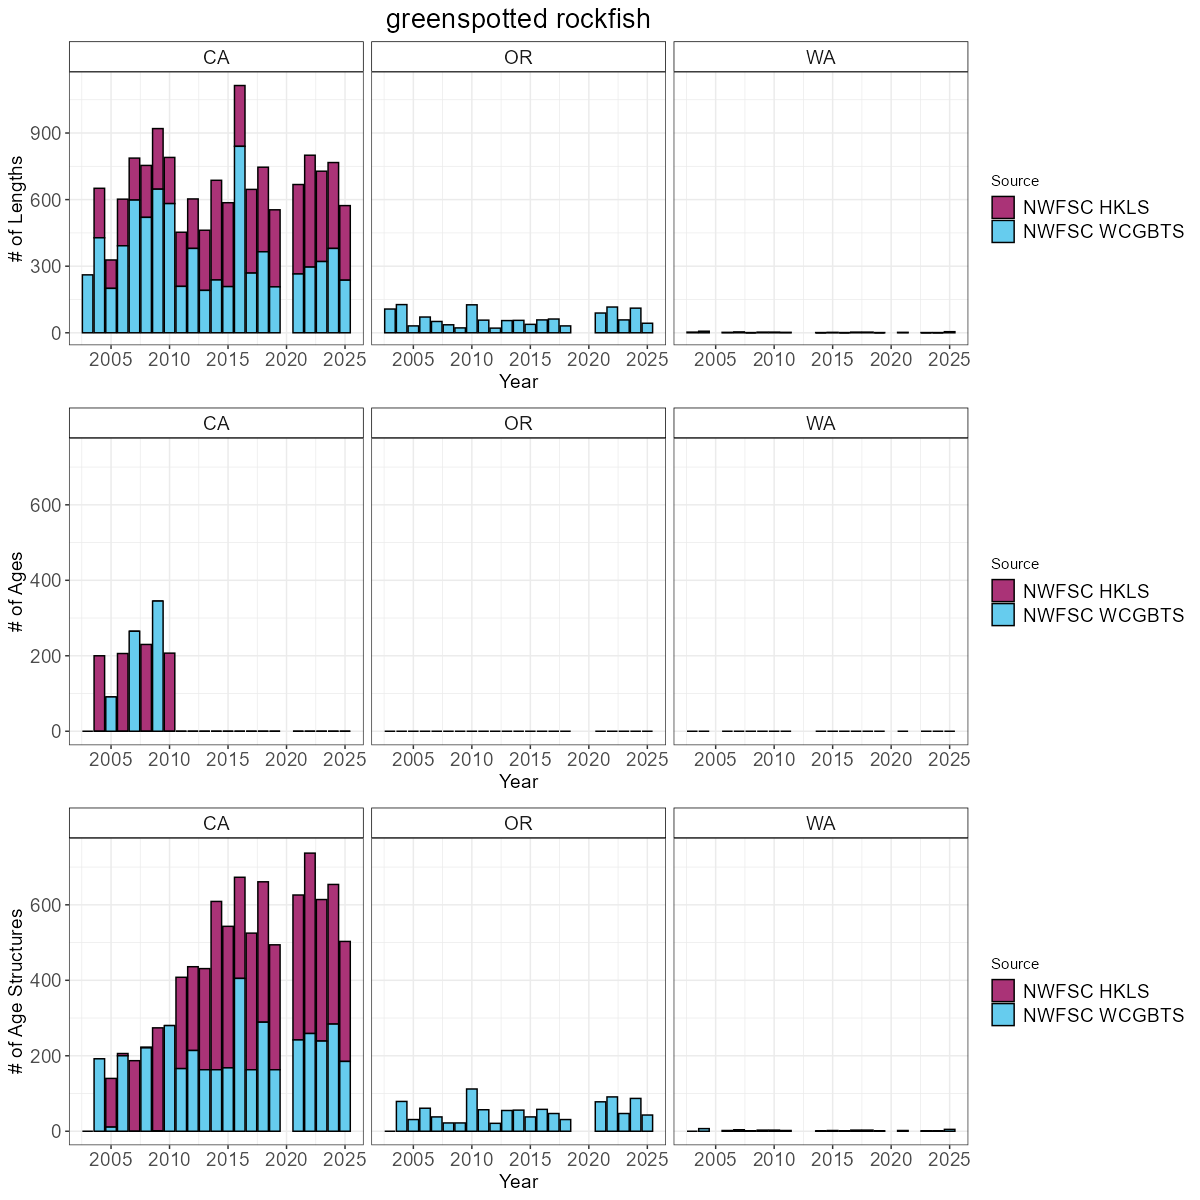
\includegraphics[keepaspectratio]{../plots/state_comparisons/greenspotted_rockfish_state_compositions.png}}

}

\caption{Total number of available lengths, read ages, and unread age
structures by data source by year. Note the y-axis is unique for the
number of lengths plot row compared to the number of age and age
structure plot rows.}

\end{figure}%

\newpage{}

\subsection{Greenstriped rockfish}\label{greenstriped-rockfish}

The most recent assessment of greenstriped rockfish was a benchmark
assessment conducted in 2009. Across available data, greenstriped
rockfish have been observed and sampled by both the NWFSC WCGBT and HKL
surveys. The NWFSC HKL survey has an average of 25 positive tows per
year. The NWFSC WCGBTS survey has an average of 154 positive tows per
year. Across the coast a total of 73 maturity samples have been
collected with 73 read maturities.

\begingroup\fontsize{10}{12}\selectfont
\begingroup\fontsize{10}{12}\selectfont

\begin{longtable}[t]{>{\raggedleft\arraybackslash}p{2cm}>{\raggedleft\arraybackslash}p{3.5cm}>{\raggedleft\arraybackslash}p{2cm}>{\raggedleft\arraybackslash}p{2cm}>{\raggedleft\arraybackslash}p{2cm}}
\caption{\label{tab:unnamed-chunk-76}Total number of available lengths, read ages, and unread age structures by data source and
state between for greenstriped rockfish.}\\
\toprule
State & Source & Lengths & Ages & Age Structures\\
\midrule
\endfirsthead
\caption[]{Total number of available lengths, read ages, and unread age structures by data source and
state between for greenstriped rockfish. (\textit{continued)}}\\
\toprule
State & Source & Lengths & Ages & Age Structures\\
\midrule
\endhead

\endfoot
\bottomrule
\endlastfoot
CA & NWFSC HKL & 1,180 & 0 & 1,167\\
CA & NWFSC WCGBTS & 16,867 & 1,359 & 4,220\\
OR & NWFSC WCGBTS & 19,607 & 1,346 & 3,924\\
WA & NWFSC WCGBTS & 10,355 & 709 & 1,918\\*
\end{longtable}
\endgroup{}
\endgroup{}

\begin{figure}[H]

{\centering \pandocbounded{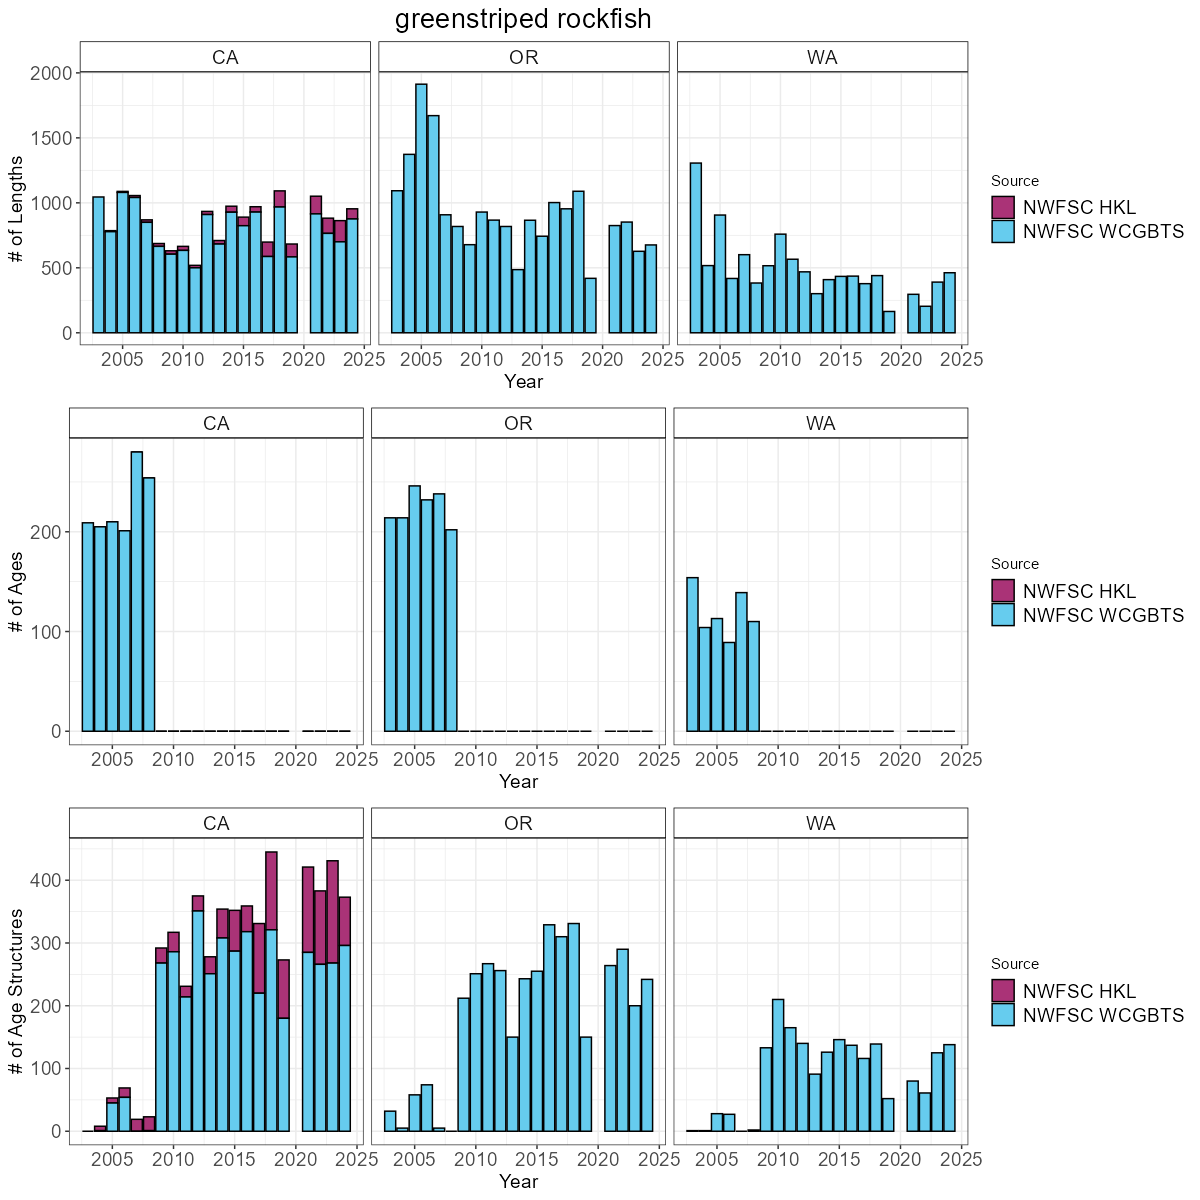
\includegraphics[keepaspectratio]{../plots/state_comparisons/greenstriped_rockfish_state_compositions.png}}

}

\caption{Total number of available lengths, read ages, and unread age
structures by data source by year. Note the y-axis is unique for the
number of lengths plot row compared to the number of age and age
structure plot rows.}

\end{figure}%

\newpage{}

\subsection{Kelp greenling}\label{kelp-greenling}

The most recent assessment of kelp greenling was a benchmark assessment
conducted in 2015. Across available data, kelp greenling have been
observed and sampled by the NWFSC WCGBT survey. The NWFSC WCGBTS survey
has an average of 9 positive tows per year. Across the coast a total of
8 maturity samples have been collected with 8 read maturities. ODFW
scientists have conducted research looking at the influences of hypoxia
on the catch per unit effort for kelp greenling.

\begingroup\fontsize{10}{12}\selectfont
\begingroup\fontsize{10}{12}\selectfont

\begin{longtable}[t]{>{\raggedleft\arraybackslash}p{2cm}>{\raggedleft\arraybackslash}p{3.5cm}>{\raggedleft\arraybackslash}p{2cm}>{\raggedleft\arraybackslash}p{2cm}>{\raggedleft\arraybackslash}p{2cm}}
\caption{\label{tab:unnamed-chunk-81}Total number of available lengths, read ages, and unread age structures by data source and
state between for kelp greenling.}\\
\toprule
State & Source & Lengths & Ages & Age Structures\\
\midrule
\endfirsthead
\caption[]{Total number of available lengths, read ages, and unread age structures by data source and
state between for kelp greenling. (\textit{continued)}}\\
\toprule
State & Source & Lengths & Ages & Age Structures\\
\midrule
\endhead

\endfoot
\bottomrule
\endlastfoot
OR & NWFSC WCGBTS & 673 & 0 & 504\\
WA & NWFSC WCGBTS & 214 & 0 & 194\\*
\end{longtable}
\endgroup{}
\endgroup{}

\begin{figure}[H]

{\centering \pandocbounded{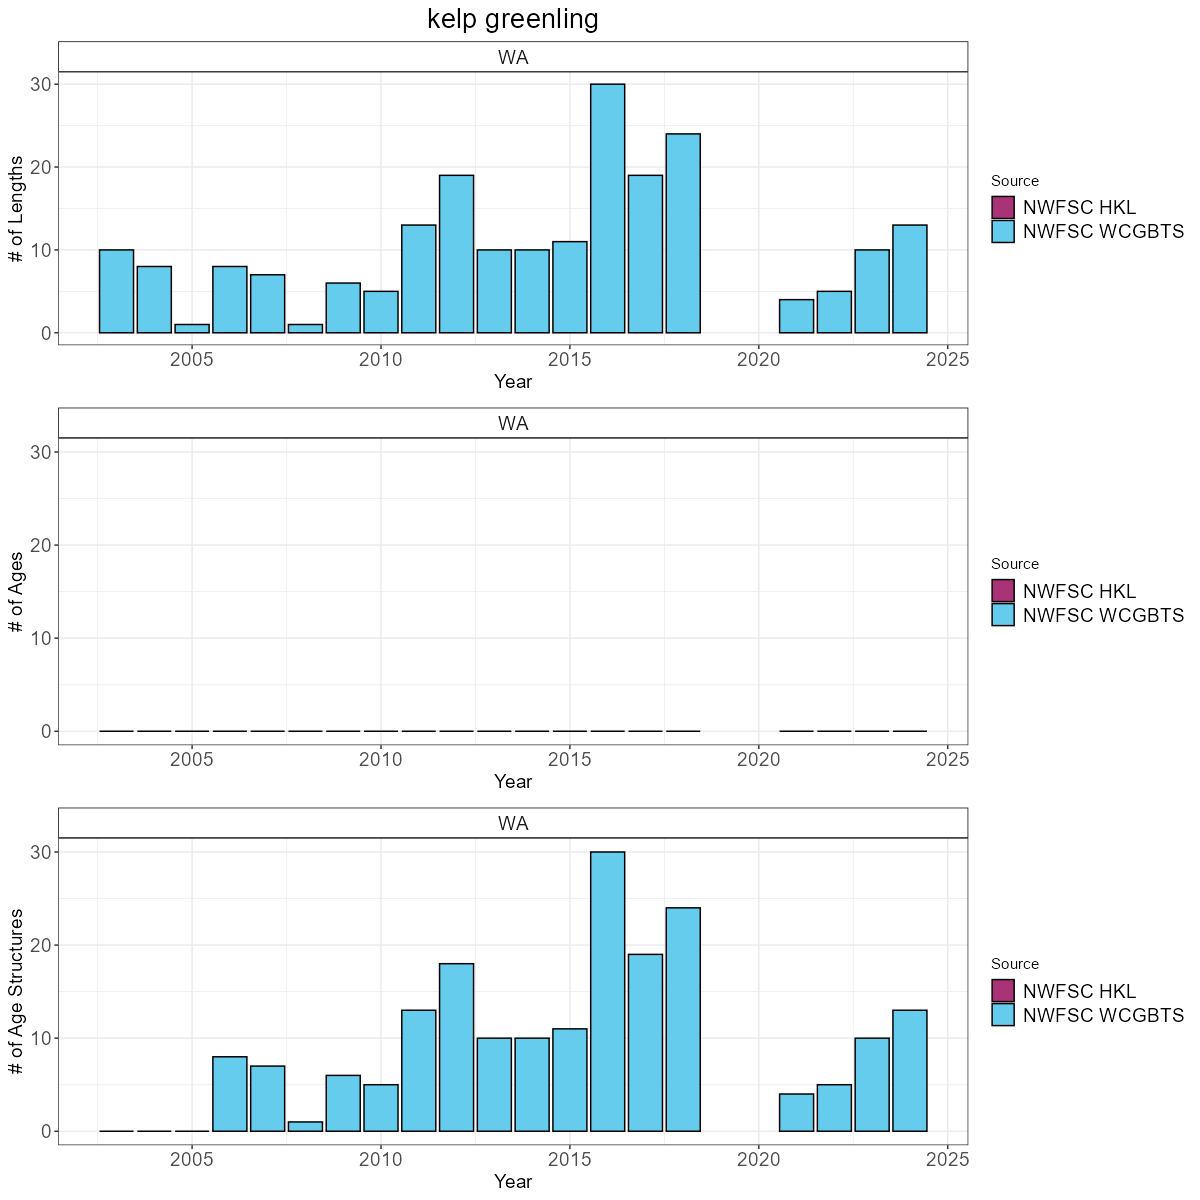
\includegraphics[keepaspectratio]{../plots/state_comparisons/kelp_greenling_state_compositions.png}}

}

\caption{Total number of available lengths, read ages, and unread age
structures by data source by year. Note the y-axis is unique for the
number of lengths plot row compared to the number of age and age
structure plot rows.}

\end{figure}%

\newpage{}

\subsection{Lingcod north}\label{lingcod-north}

The most recent assessment of lingcod north was a benchmark assessment
conducted in 2021. Across available data, lingcod north have been
observed and sampled by the NWFSC WCGBT survey. The NWFSC WCGBTS survey
has an average of 124 positive tows per year. Across the coast a total
of 1161 maturity samples have been collected with 1031 read maturities.
ODFW scientists have conducted research looking at the influences of
hypoxia on the catch per unit effort for lingcod north.

\begingroup\fontsize{10}{12}\selectfont
\begingroup\fontsize{10}{12}\selectfont

\begin{longtable}[t]{>{\raggedleft\arraybackslash}p{2cm}>{\raggedleft\arraybackslash}p{3.5cm}>{\raggedleft\arraybackslash}p{2cm}>{\raggedleft\arraybackslash}p{2cm}>{\raggedleft\arraybackslash}p{2cm}}
\caption{\label{tab:unnamed-chunk-86}Total number of available lengths, read ages, and unread age structures by data source and
state between for lingcod north.}\\
\toprule
State & Source & Lengths & Ages & Age Structures\\
\midrule
\endfirsthead
\caption[]{Total number of available lengths, read ages, and unread age structures by data source and
state between for lingcod north. (\textit{continued)}}\\
\toprule
State & Source & Lengths & Ages & Age Structures\\
\midrule
\endhead

\endfoot
\bottomrule
\endlastfoot
CA & NWFSC WCGBTS & 2,523 & 780 & 597\\
OR & NWFSC WCGBTS & 9,519 & 2,782 & 2,524\\
WA & NWFSC WCGBTS & 6,684 & 1,582 & 1,345\\*
\end{longtable}
\endgroup{}
\endgroup{}

\begin{figure}[H]

{\centering \pandocbounded{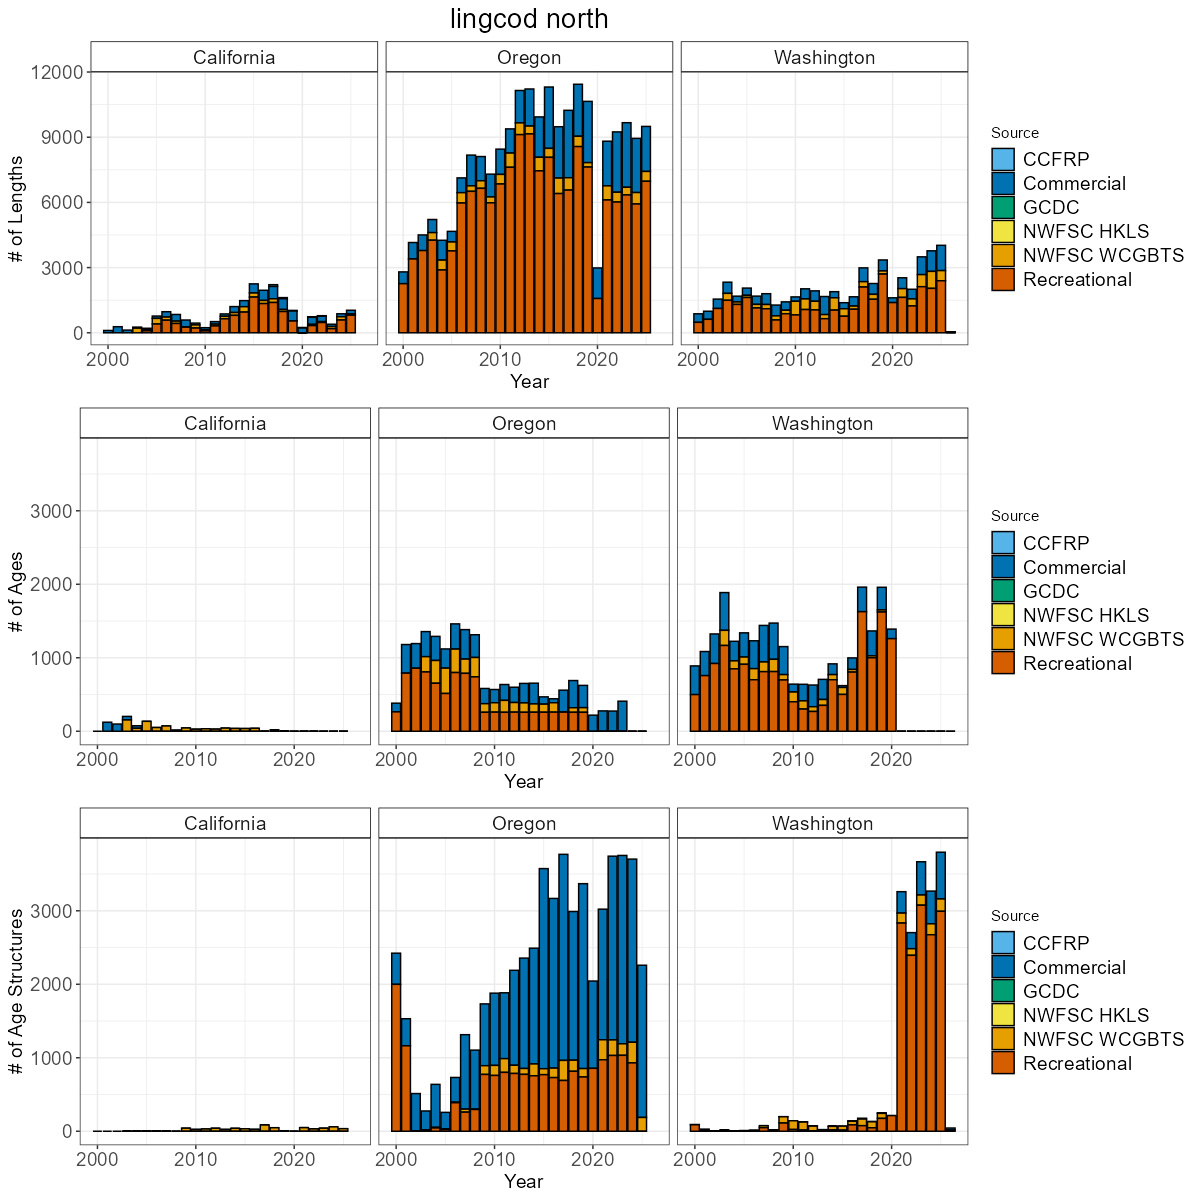
\includegraphics[keepaspectratio]{../plots/state_comparisons/lingcod_north_state_compositions.png}}

}

\caption{Total number of available lengths, read ages, and unread age
structures by data source by year. Note the y-axis is unique for the
number of lengths plot row compared to the number of age and age
structure plot rows.}

\end{figure}%

\newpage{}

\subsection{Lingcod south}\label{lingcod-south}

The most recent assessment of lingcod south was a benchmark assessment
conducted in 2021. Across available data, lingcod south have been
observed and sampled by the NWFSC WCGBT survey. The NWFSC WCGBTS survey
has an average of 75 positive tows per year. Across the coast a total of
1161 maturity samples have been collected with 1031 read maturities.

\begingroup\fontsize{10}{12}\selectfont
\begingroup\fontsize{10}{12}\selectfont

\begin{longtable}[t]{>{\raggedleft\arraybackslash}p{2cm}>{\raggedleft\arraybackslash}p{3.5cm}>{\raggedleft\arraybackslash}p{2cm}>{\raggedleft\arraybackslash}p{2cm}>{\raggedleft\arraybackslash}p{2cm}}
\caption{\label{tab:unnamed-chunk-91}Total number of available lengths, read ages, and unread age structures by data source and
state between for lingcod south.}\\
\toprule
State & Source & Lengths & Ages & Age Structures\\
\midrule
\endfirsthead
\caption[]{Total number of available lengths, read ages, and unread age structures by data source and
state between for lingcod south. (\textit{continued)}}\\
\toprule
State & Source & Lengths & Ages & Age Structures\\
\midrule
\endhead

\endfoot
\bottomrule
\endlastfoot
CA & NWFSC WCGBTS & 11,921 & 3,870 & 2,491\\*
\end{longtable}
\endgroup{}
\endgroup{}

\begin{figure}[H]

{\centering \pandocbounded{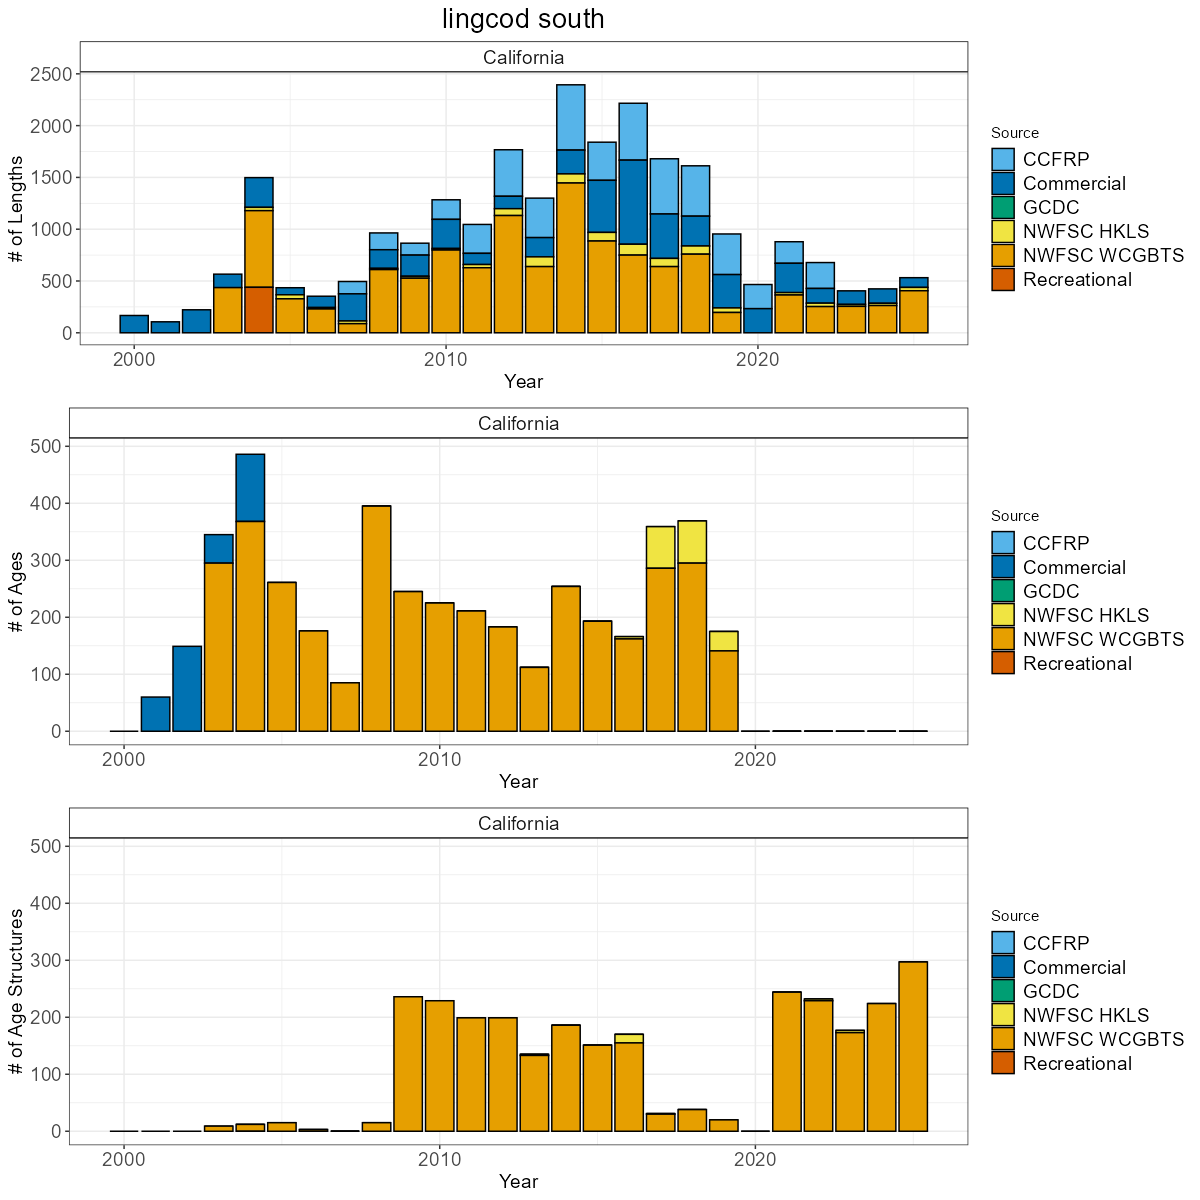
\includegraphics[keepaspectratio]{../plots/state_comparisons/lingcod_south_state_compositions.png}}

}

\caption{Total number of available lengths, read ages, and unread age
structures by data source by year. Note the y-axis is unique for the
number of lengths plot row compared to the number of age and age
structure plot rows.}

\end{figure}%

\newpage{}

\subsection{Longnose skate}\label{longnose-skate}

The most recent assessment of longnose skate was a benchmark assessment
conducted in 2019. Across available data, longnose skate have been
observed and sampled by the NWFSC WCGBT survey. The NWFSC WCGBTS survey
has an average of 364 positive tows per year. Across the coast a total
of 508 maturity samples have been collected with 508 read maturities.

\begingroup\fontsize{10}{12}\selectfont
\begingroup\fontsize{10}{12}\selectfont

\begin{longtable}[t]{>{\raggedleft\arraybackslash}p{2cm}>{\raggedleft\arraybackslash}p{3.5cm}>{\raggedleft\arraybackslash}p{2cm}>{\raggedleft\arraybackslash}p{2cm}>{\raggedleft\arraybackslash}p{2cm}}
\caption{\label{tab:unnamed-chunk-96}Total number of available lengths, read ages, and unread age structures by data source and
state between for longnose skate.}\\
\toprule
State & Source & Lengths & Ages & Age Structures\\
\midrule
\endfirsthead
\caption[]{Total number of available lengths, read ages, and unread age structures by data source and
state between for longnose skate. (\textit{continued)}}\\
\toprule
State & Source & Lengths & Ages & Age Structures\\
\midrule
\endhead

\endfoot
\bottomrule
\endlastfoot
CA & NWFSC WCGBTS & 34,520 & 336 & 1,229\\
OR & NWFSC WCGBTS & 18,099 & 227 & 850\\
WA & NWFSC WCGBTS & 8,858 & 84 & 347\\*
\end{longtable}
\endgroup{}
\endgroup{}

\begin{figure}[H]

{\centering \pandocbounded{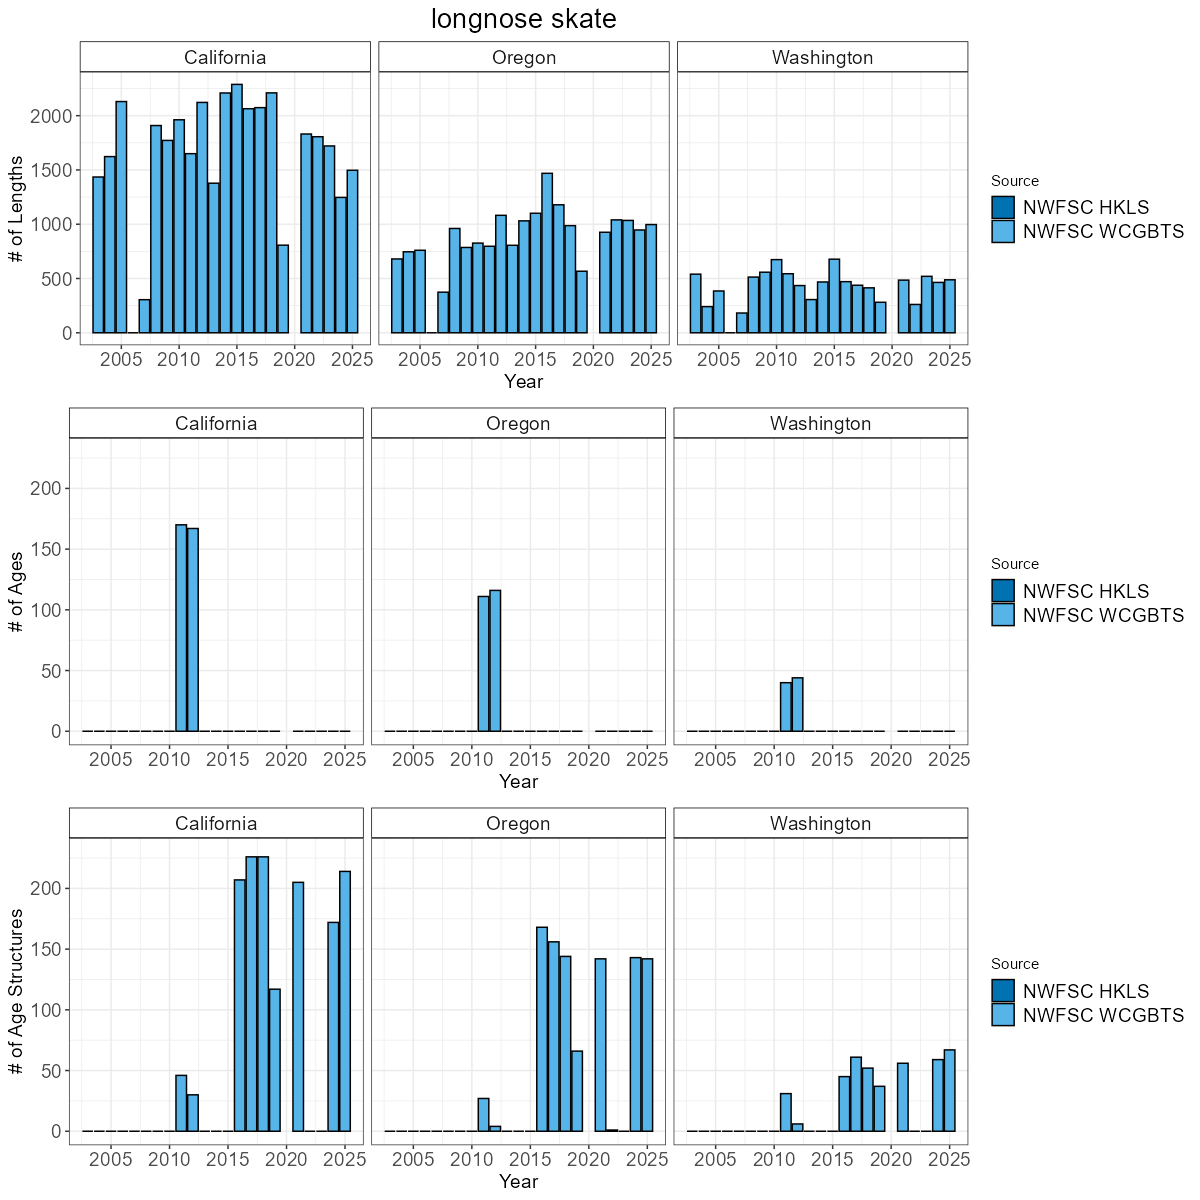
\includegraphics[keepaspectratio]{../plots/state_comparisons/longnose_skate_state_compositions.png}}

}

\caption{Total number of available lengths, read ages, and unread age
structures by data source by year. Note the y-axis is unique for the
number of lengths plot row compared to the number of age and age
structure plot rows.}

\end{figure}%

\newpage{}

\subsection{Longspine thornyhead}\label{longspine-thornyhead}

The most recent assessment of longspine thornyhead was a benchmark
assessment conducted in 2013. Across available data, longspine
thornyhead have been observed and sampled by the NWFSC WCGBT survey. The
NWFSC WCGBTS survey has an average of 211 positive tows per year. Across
the coast a total of 341 maturity samples have been collected with 63
read maturities.

\begingroup\fontsize{10}{12}\selectfont
\begingroup\fontsize{10}{12}\selectfont

\begin{longtable}[t]{>{\raggedleft\arraybackslash}p{2cm}>{\raggedleft\arraybackslash}p{3.5cm}>{\raggedleft\arraybackslash}p{2cm}>{\raggedleft\arraybackslash}p{2cm}>{\raggedleft\arraybackslash}p{2cm}}
\caption{\label{tab:unnamed-chunk-101}Total number of available lengths, read ages, and unread age structures by data source and
state between for longspine thornyhead.}\\
\toprule
State & Source & Lengths & Ages & Age Structures\\
\midrule
\endfirsthead
\caption[]{Total number of available lengths, read ages, and unread age structures by data source and
state between for longspine thornyhead. (\textit{continued)}}\\
\toprule
State & Source & Lengths & Ages & Age Structures\\
\midrule
\endhead

\endfoot
\bottomrule
\endlastfoot
CA & NWFSC WCGBTS & 73,218 & 0 & 9,607\\
OR & NWFSC WCGBTS & 33,808 & 0 & 4,111\\
WA & NWFSC WCGBTS & 14,270 & 0 & 1,777\\*
\end{longtable}
\endgroup{}
\endgroup{}

\begin{figure}[H]

{\centering \pandocbounded{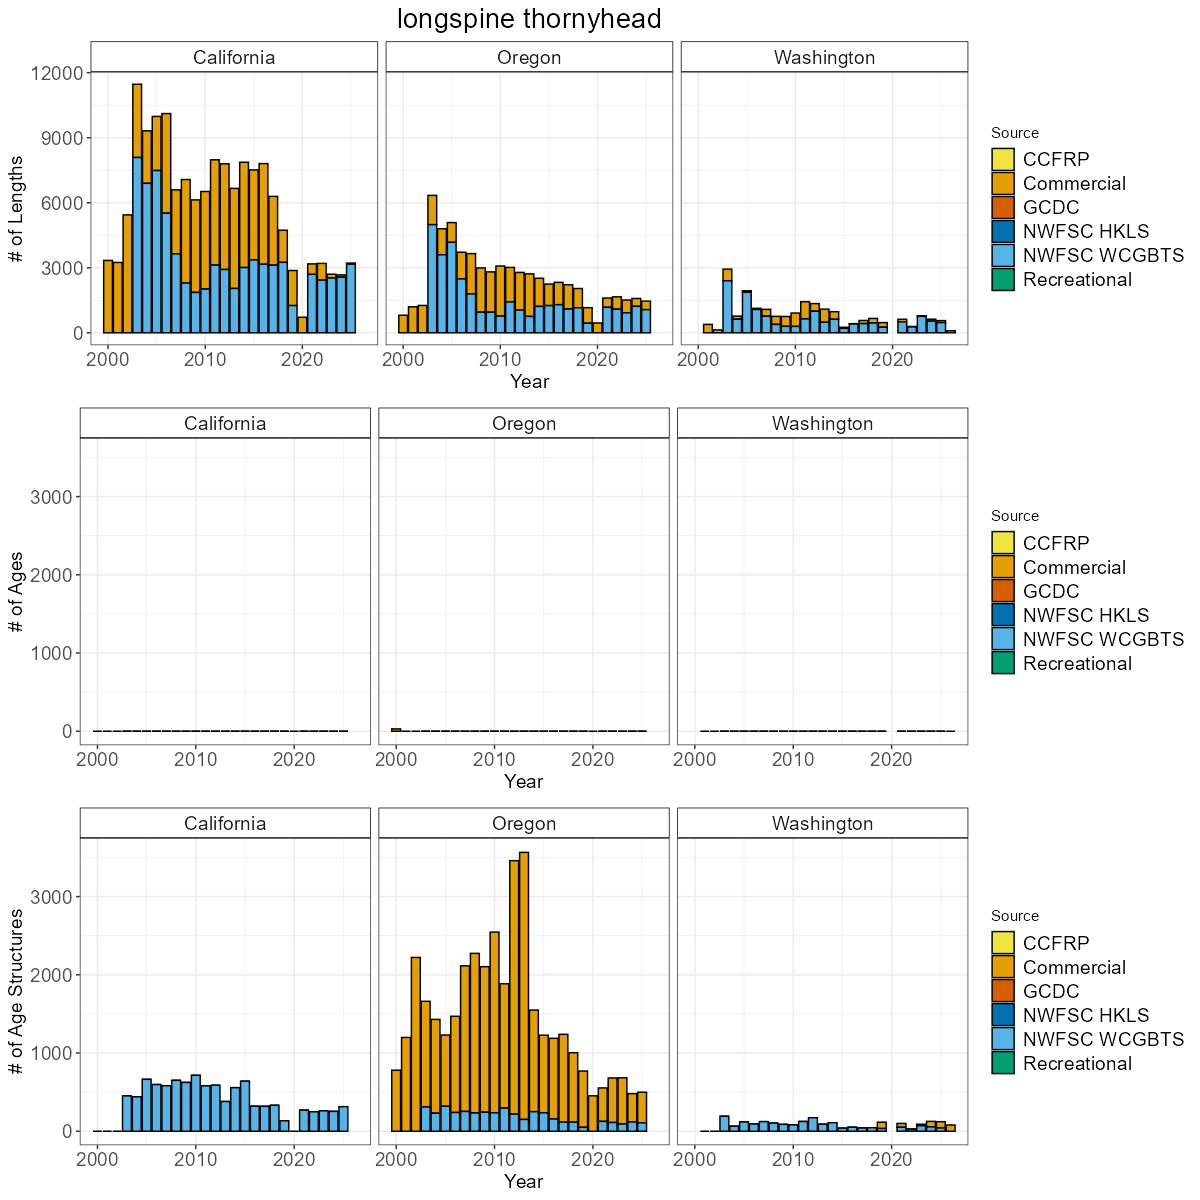
\includegraphics[keepaspectratio]{../plots/state_comparisons/longspine_thornyhead_state_compositions.png}}

}

\caption{Total number of available lengths, read ages, and unread age
structures by data source by year. Note the y-axis is unique for the
number of lengths plot row compared to the number of age and age
structure plot rows.}

\end{figure}%

\newpage{}

\subsection{Pacific cod}\label{pacific-cod}

To date, no assessment or analysis has been conducted on Pacific cod.
Across available data, Pacific cod have been observed and sampled by the
NWFSC WCGBT survey. The NWFSC WCGBTS survey has an average of 27
positive tows per year. Across the coast a total of 125 maturity samples
have been collected with 0 read maturities.

\begingroup\fontsize{10}{12}\selectfont
\begingroup\fontsize{10}{12}\selectfont

\begin{longtable}[t]{>{\raggedleft\arraybackslash}p{2cm}>{\raggedleft\arraybackslash}p{3.5cm}>{\raggedleft\arraybackslash}p{2cm}>{\raggedleft\arraybackslash}p{2cm}>{\raggedleft\arraybackslash}p{2cm}}
\caption{\label{tab:unnamed-chunk-106}Total number of available lengths, read ages, and unread age structures by data source and
state between for Pacific cod.}\\
\toprule
State & Source & Lengths & Ages & Age Structures\\
\midrule
\endfirsthead
\caption[]{Total number of available lengths, read ages, and unread age structures by data source and
state between for Pacific cod. (\textit{continued)}}\\
\toprule
State & Source & Lengths & Ages & Age Structures\\
\midrule
\endhead

\endfoot
\bottomrule
\endlastfoot
CA & NWFSC WCGBTS & 14 & 0 & 0\\
OR & NWFSC WCGBTS & 511 & 0 & 215\\
WA & NWFSC WCGBTS & 3,747 & 0 & 1,342\\*
\end{longtable}
\endgroup{}
\endgroup{}

\begin{figure}[H]

{\centering \pandocbounded{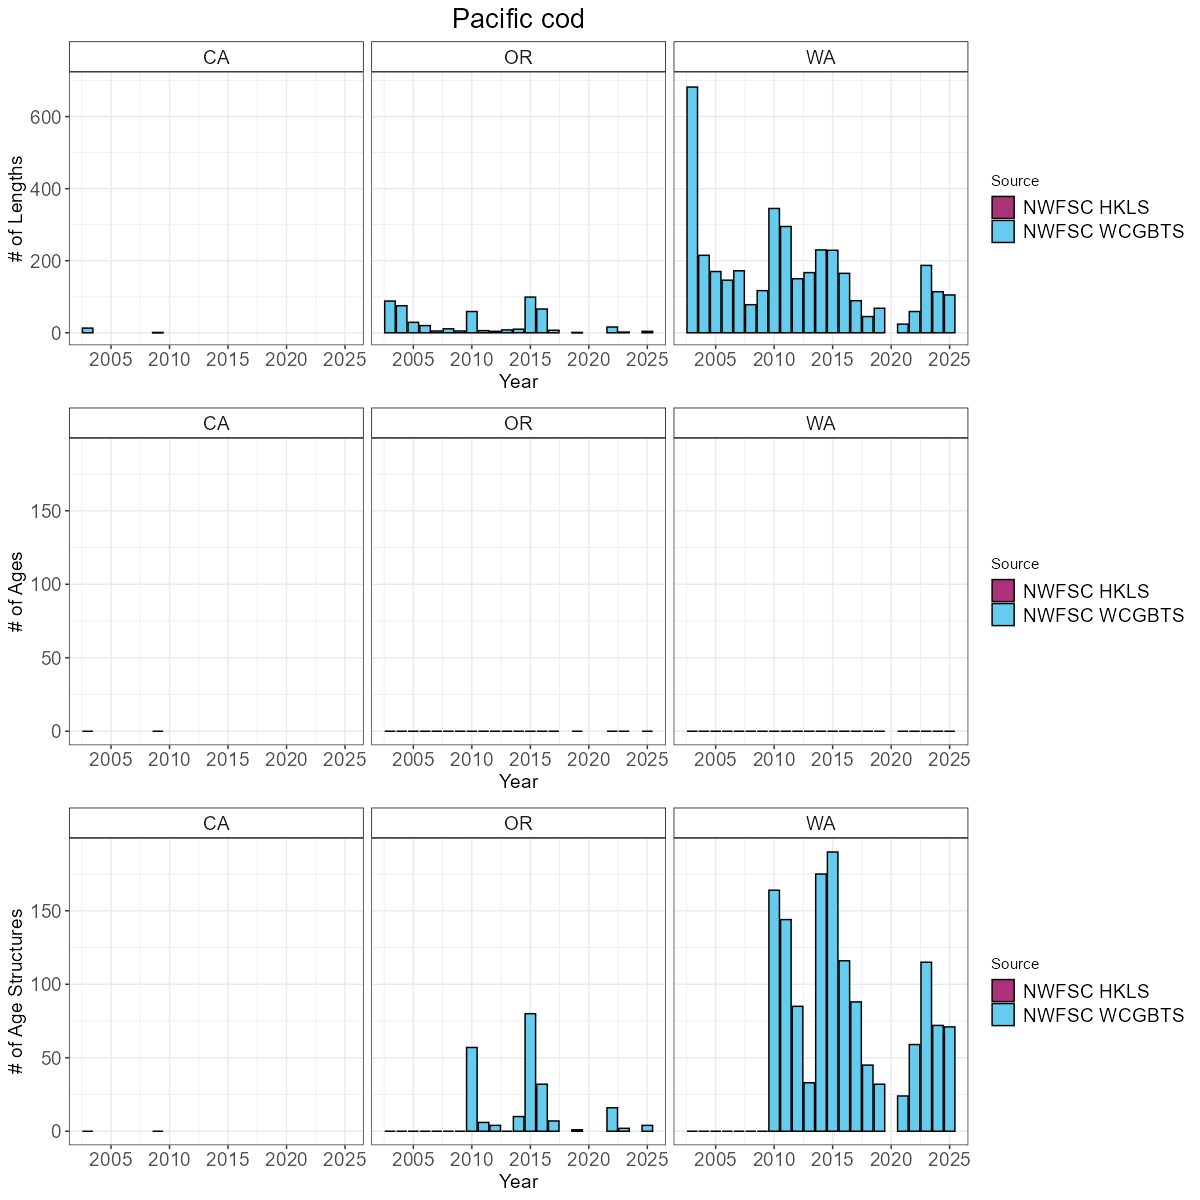
\includegraphics[keepaspectratio]{../plots/state_comparisons/pacific_cod_state_compositions.png}}

}

\caption{Total number of available lengths, read ages, and unread age
structures by data source by year. Note the y-axis is unique for the
number of lengths plot row compared to the number of age and age
structure plot rows.}

\end{figure}%

\newpage{}

\subsection{Pacific ocean perch}\label{pacific-ocean-perch}

The most recent assessment of Pacific ocean perch was a benchmark
assessment conducted in 2017. Across available data, Pacific ocean perch
have been observed and sampled by the NWFSC WCGBT survey. The NWFSC
WCGBTS survey has an average of 46 positive tows per year. Across the
coast a total of 583 maturity samples have been collected with 583 read
maturities.

\begingroup\fontsize{10}{12}\selectfont
\begingroup\fontsize{10}{12}\selectfont

\begin{longtable}[t]{>{\raggedleft\arraybackslash}p{2cm}>{\raggedleft\arraybackslash}p{3.5cm}>{\raggedleft\arraybackslash}p{2cm}>{\raggedleft\arraybackslash}p{2cm}>{\raggedleft\arraybackslash}p{2cm}}
\caption{\label{tab:unnamed-chunk-111}Total number of available lengths, read ages, and unread age structures by data source and
state between for Pacific ocean perch.}\\
\toprule
State & Source & Lengths & Ages & Age Structures\\
\midrule
\endfirsthead
\caption[]{Total number of available lengths, read ages, and unread age structures by data source and
state between for Pacific ocean perch. (\textit{continued)}}\\
\toprule
State & Source & Lengths & Ages & Age Structures\\
\midrule
\endhead

\endfoot
\bottomrule
\endlastfoot
CA & NWFSC WCGBTS & 232 & 78 & 153\\
OR & NWFSC WCGBTS & 9,520 & 3,061 & 3,776\\
WA & NWFSC WCGBTS & 8,009 & 2,743 & 1,955\\*
\end{longtable}
\endgroup{}
\endgroup{}

\begin{figure}[H]

{\centering \pandocbounded{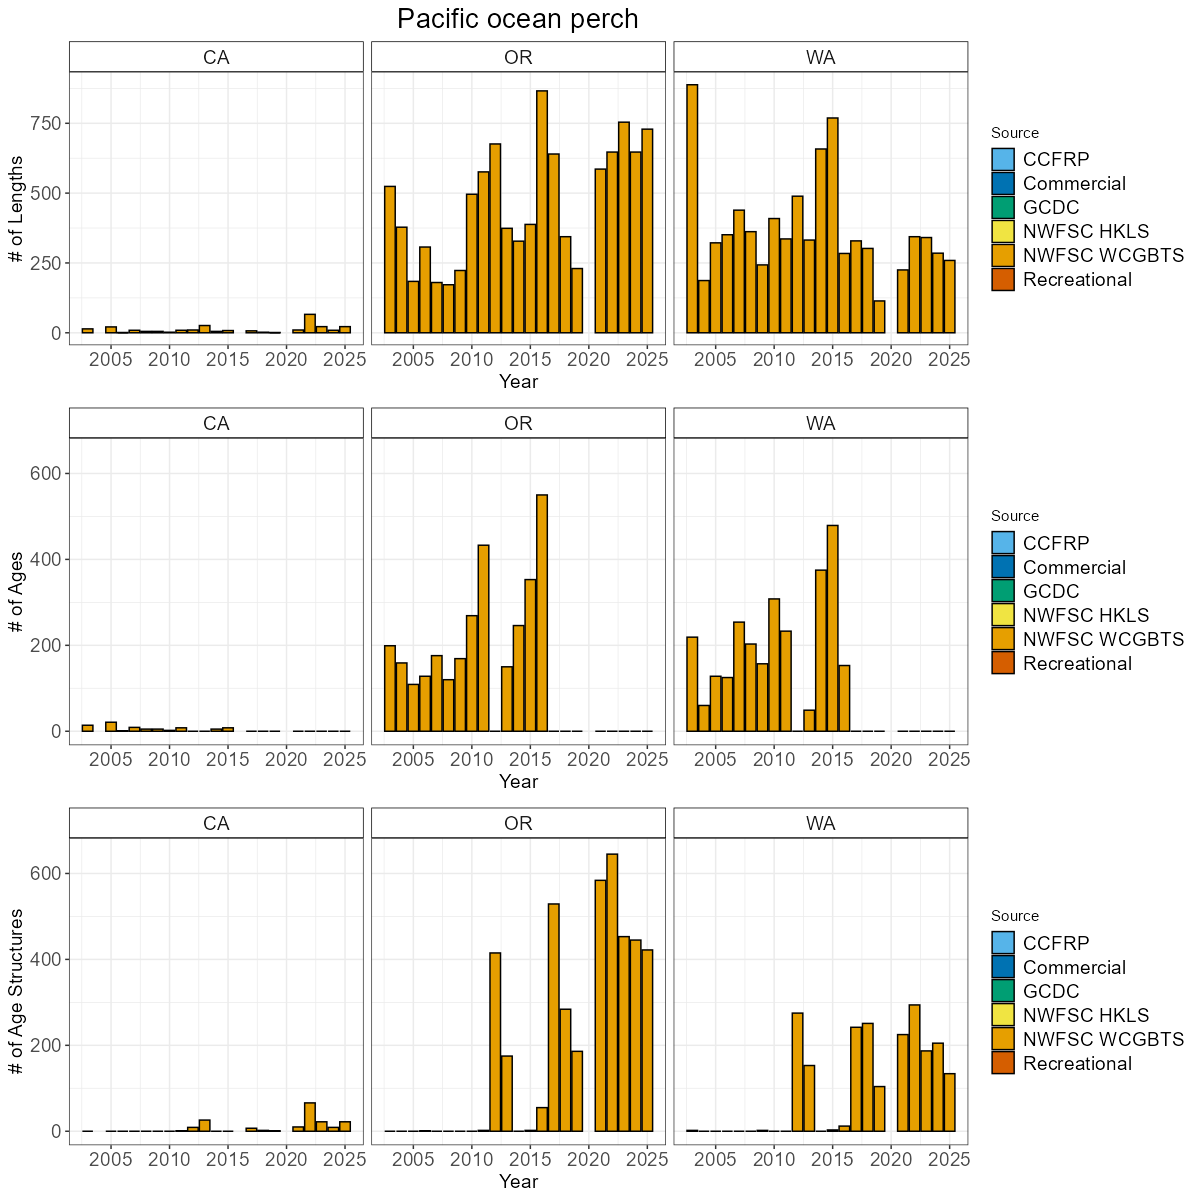
\includegraphics[keepaspectratio]{../plots/state_comparisons/pacific_ocean_perch_state_compositions.png}}

}

\caption{Total number of available lengths, read ages, and unread age
structures by data source by year. Note the y-axis is unique for the
number of lengths plot row compared to the number of age and age
structure plot rows.}

\end{figure}%

\newpage{}

\subsection{Pacific sanddab}\label{pacific-sanddab}

To date, no assessment or analysis has been conducted on Pacific
sanddab. Across available data, Pacific sanddab have been observed and
sampled by the NWFSC WCGBT survey. The NWFSC WCGBTS survey has an
average of 198 positive tows per year. Across the coast a total of 0
maturity samples have been collected with 0 read maturities.

\begingroup\fontsize{10}{12}\selectfont
\begingroup\fontsize{10}{12}\selectfont

\begin{longtable}[t]{>{\raggedleft\arraybackslash}p{2cm}>{\raggedleft\arraybackslash}p{3.5cm}>{\raggedleft\arraybackslash}p{2cm}>{\raggedleft\arraybackslash}p{2cm}>{\raggedleft\arraybackslash}p{2cm}}
\caption{\label{tab:unnamed-chunk-116}Total number of available lengths, read ages, and unread age structures by data source and
state between for Pacific sanddab.}\\
\toprule
State & Source & Lengths & Ages & Age Structures\\
\midrule
\endfirsthead
\caption[]{Total number of available lengths, read ages, and unread age structures by data source and
state between for Pacific sanddab. (\textit{continued)}}\\
\toprule
State & Source & Lengths & Ages & Age Structures\\
\midrule
\endhead

\endfoot
\bottomrule
\endlastfoot
CA & NWFSC WCGBTS & 53,720 & 4,714 & 3,943\\
OR & NWFSC WCGBTS & 27,649 & 2,374 & 2,175\\
WA & NWFSC WCGBTS & 10,581 & 874 & 903\\*
\end{longtable}
\endgroup{}
\endgroup{}

\begin{figure}[H]

{\centering \pandocbounded{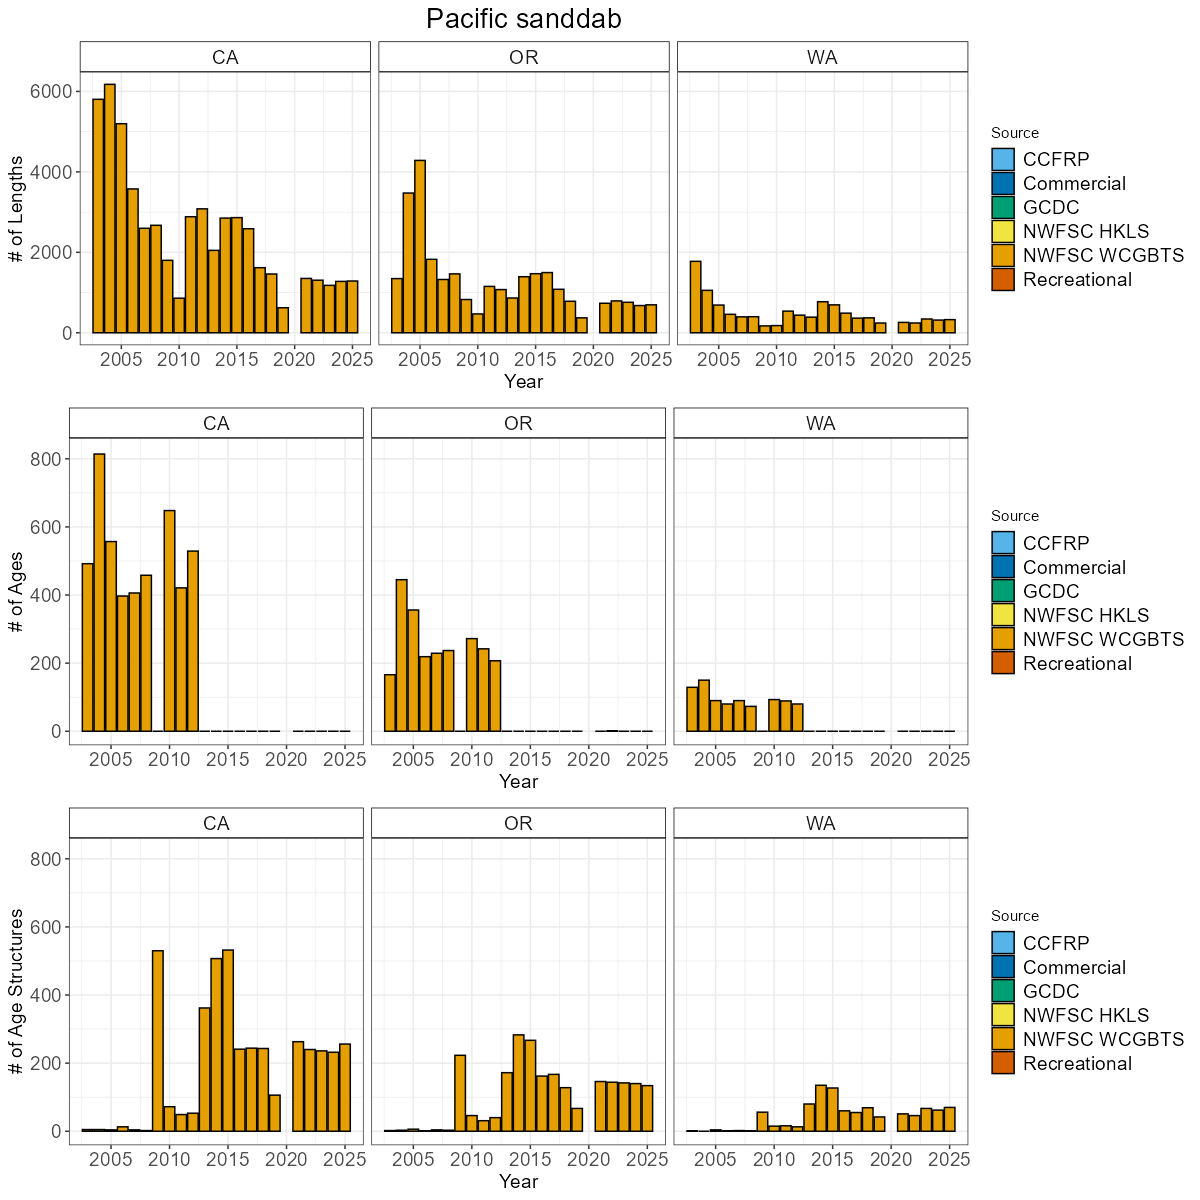
\includegraphics[keepaspectratio]{../plots/state_comparisons/pacific_sanddab_state_compositions.png}}

}

\caption{Total number of available lengths, read ages, and unread age
structures by data source by year. Note the y-axis is unique for the
number of lengths plot row compared to the number of age and age
structure plot rows.}

\end{figure}%

\newpage{}

\subsection{Pacific spiny dogfish}\label{pacific-spiny-dogfish}

The most recent assessment of Pacific spiny dogfish was a benchmark
assessment conducted in 2021. Across available data, Pacific spiny
dogfish have been observed and sampled by the NWFSC WCGBT survey. The
NWFSC WCGBTS survey has an average of 155 positive tows per year. Across
the coast a total of 0 maturity samples have been collected with 0 read
maturities. Researchers have conducted an analysis of the trends of
Pacific spiny dogfish across the North Pacific indicating declining
population trends across regions.

\begingroup\fontsize{10}{12}\selectfont
\begingroup\fontsize{10}{12}\selectfont

\begin{longtable}[t]{>{\raggedleft\arraybackslash}p{2cm}>{\raggedleft\arraybackslash}p{3.5cm}>{\raggedleft\arraybackslash}p{2cm}>{\raggedleft\arraybackslash}p{2cm}>{\raggedleft\arraybackslash}p{2cm}}
\caption{\label{tab:unnamed-chunk-121}Total number of available lengths, read ages, and unread age structures by data source and
state between for Pacific spiny dogfish.}\\
\toprule
State & Source & Lengths & Ages & Age Structures\\
\midrule
\endfirsthead
\caption[]{Total number of available lengths, read ages, and unread age structures by data source and
state between for Pacific spiny dogfish. (\textit{continued)}}\\
\toprule
State & Source & Lengths & Ages & Age Structures\\
\midrule
\endhead

\endfoot
\bottomrule
\endlastfoot
CA & NWFSC HKL & 7 & 0 & 0\\
CA & NWFSC WCGBTS & 17,911 & 285 & 4,744\\
OR & NWFSC WCGBTS & 4,384 & 128 & 1,879\\
WA & NWFSC WCGBTS & 11,562 & 178 & 2,877\\*
\end{longtable}
\endgroup{}
\endgroup{}

\begin{figure}[H]

{\centering \pandocbounded{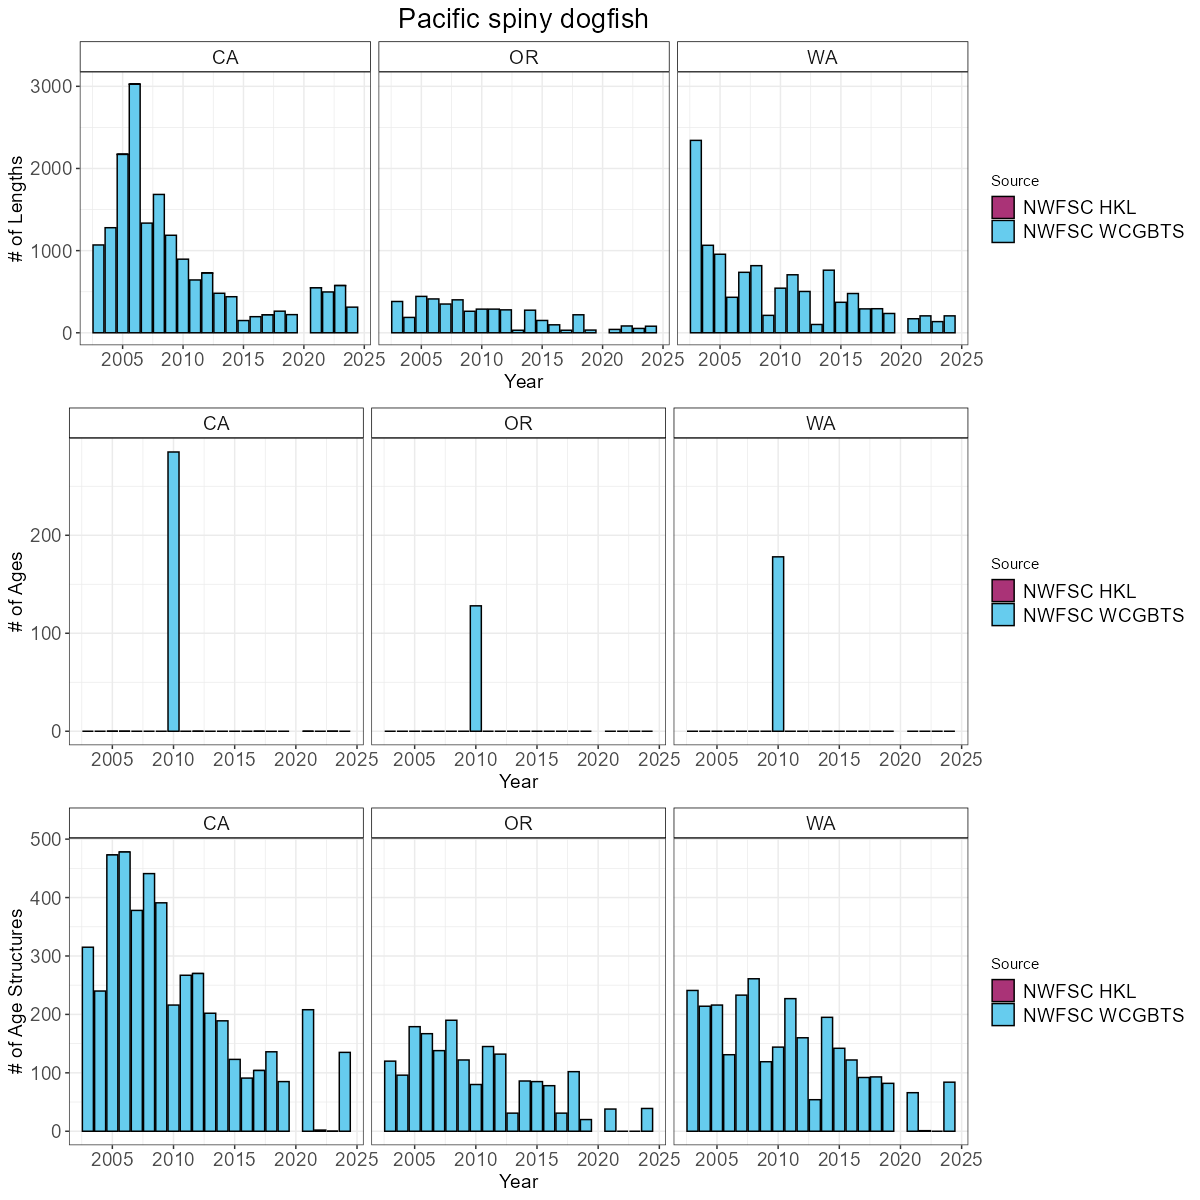
\includegraphics[keepaspectratio]{../plots/state_comparisons/pacific_spiny_dogfish_state_compositions.png}}

}

\caption{Total number of available lengths, read ages, and unread age
structures by data source by year. Note the y-axis is unique for the
number of lengths plot row compared to the number of age and age
structure plot rows.}

\end{figure}%

\newpage{}

\subsection{Petrale sole}\label{petrale-sole}

The most recent assessment of petrale sole was a benchmark assessment
conducted in 2023. Across available data, petrale sole have been
observed and sampled by the NWFSC WCGBT survey. The NWFSC WCGBTS survey
has an average of 260 positive tows per year. Across the coast a total
of 728 maturity samples have been collected with 598 read maturities.

\begingroup\fontsize{10}{12}\selectfont
\begingroup\fontsize{10}{12}\selectfont

\begin{longtable}[t]{>{\raggedleft\arraybackslash}p{2cm}>{\raggedleft\arraybackslash}p{3.5cm}>{\raggedleft\arraybackslash}p{2cm}>{\raggedleft\arraybackslash}p{2cm}>{\raggedleft\arraybackslash}p{2cm}}
\caption{\label{tab:unnamed-chunk-126}Total number of available lengths, read ages, and unread age structures by data source and
state between for petrale sole.}\\
\toprule
State & Source & Lengths & Ages & Age Structures\\
\midrule
\endfirsthead
\caption[]{Total number of available lengths, read ages, and unread age structures by data source and
state between for petrale sole. (\textit{continued)}}\\
\toprule
State & Source & Lengths & Ages & Age Structures\\
\midrule
\endhead

\endfoot
\bottomrule
\endlastfoot
CA & NWFSC HKL & 4 & 0 & 0\\
CA & NWFSC WCGBTS & 35,677 & 7,165 & 3,016\\
OR & NWFSC WCGBTS & 31,575 & 4,857 & 3,589\\
WA & NWFSC WCGBTS & 15,349 & 2,676 & 2,089\\*
\end{longtable}
\endgroup{}
\endgroup{}

\begin{figure}[H]

{\centering \pandocbounded{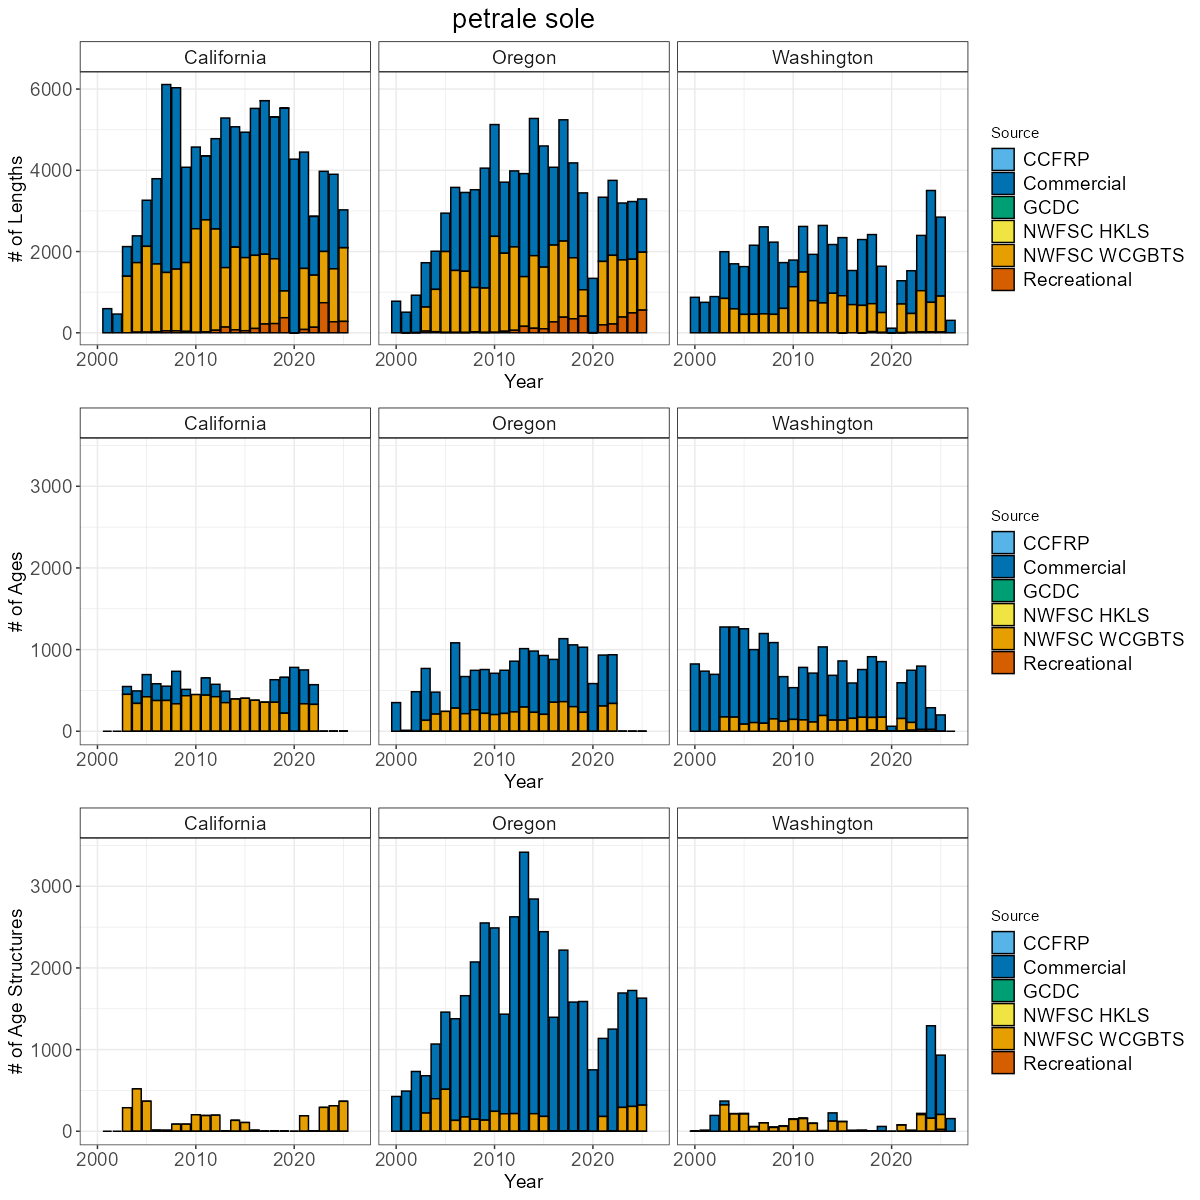
\includegraphics[keepaspectratio]{../plots/state_comparisons/petrale_sole_state_compositions.png}}

}

\caption{Total number of available lengths, read ages, and unread age
structures by data source by year. Note the y-axis is unique for the
number of lengths plot row compared to the number of age and age
structure plot rows.}

\end{figure}%

\newpage{}

\subsection{Quillback rockfish}\label{quillback-rockfish}

The most recent assessment of quillback rockfish was a data-moderate
assessment conducted in 2021. Across available data, quillback rockfish
have been observed and sampled by the NWFSC WCGBT survey. Across the
coast a total of 167 maturity samples have been collected with 162 read
maturities. ODFW scientists have conducted research looking at the
influences of hypoxia on the catch per unit effort for quillback
rockfish.

\begingroup\fontsize{10}{12}\selectfont
\begingroup\fontsize{10}{12}\selectfont

\begin{longtable}[t]{>{\raggedleft\arraybackslash}p{2cm}>{\raggedleft\arraybackslash}p{3.5cm}>{\raggedleft\arraybackslash}p{2cm}>{\raggedleft\arraybackslash}p{2cm}>{\raggedleft\arraybackslash}p{2cm}}
\caption{\label{tab:unnamed-chunk-131}Total number of available lengths, read ages, and unread age structures by data source and
state between for quillback rockfish.}\\
\toprule
State & Source & Lengths & Ages & Age Structures\\
\midrule
\endfirsthead
\caption[]{Total number of available lengths, read ages, and unread age structures by data source and
state between for quillback rockfish. (\textit{continued)}}\\
\toprule
State & Source & Lengths & Ages & Age Structures\\
\midrule
\endhead

\endfoot
\bottomrule
\endlastfoot
OR & NWFSC WCGBTS & 124 & 87 & 20\\
WA & NWFSC WCGBTS & 105 & 75 & 9\\*
\end{longtable}
\endgroup{}
\endgroup{}

\begin{figure}[H]

{\centering \pandocbounded{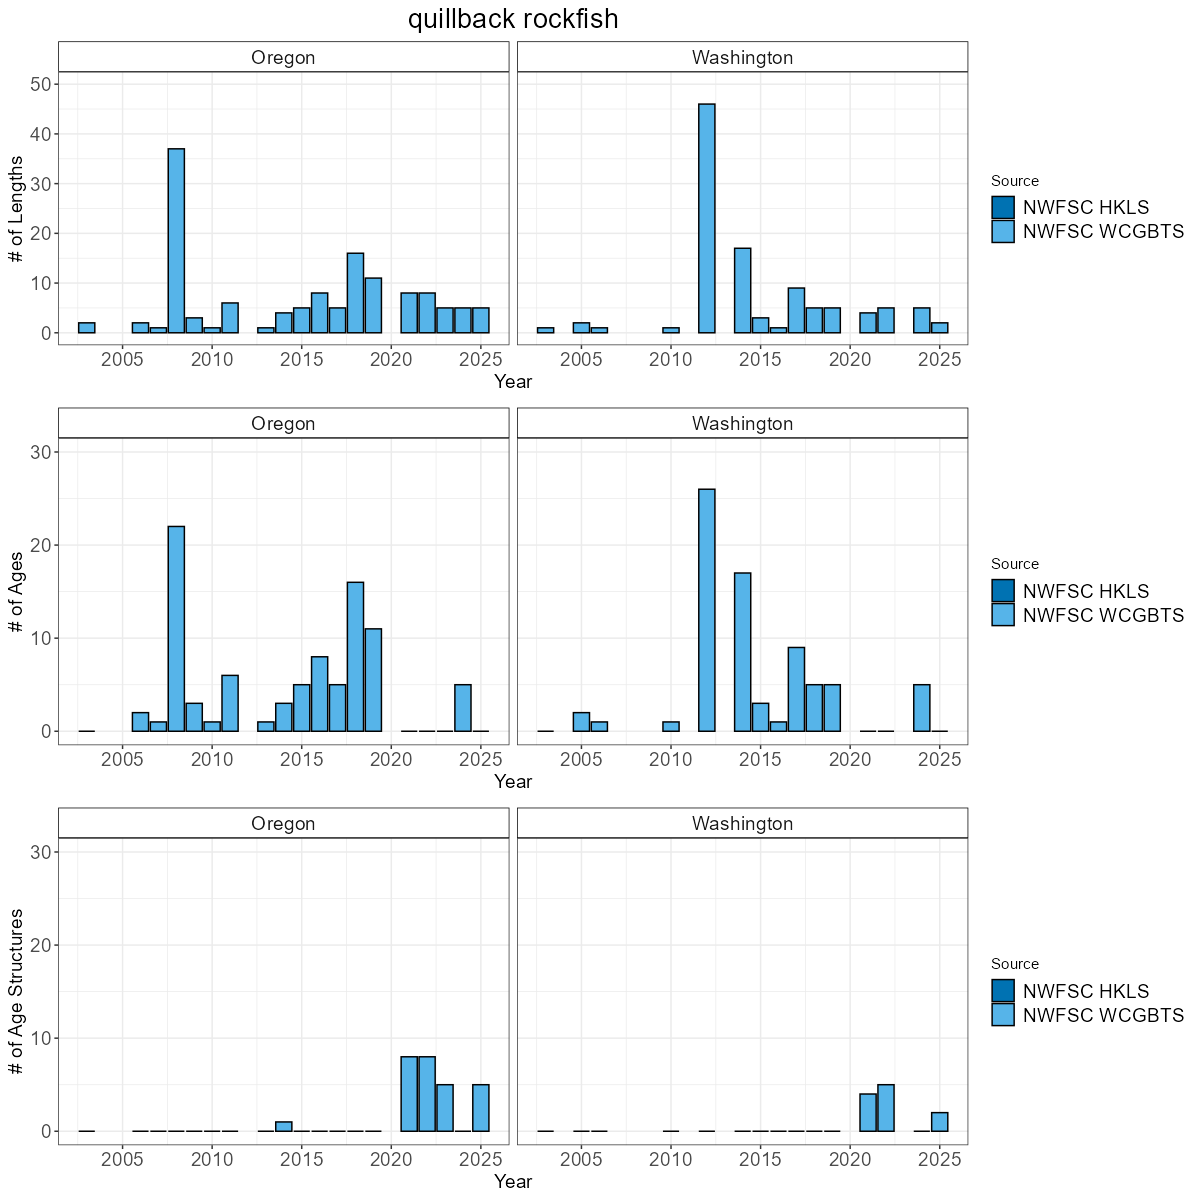
\includegraphics[keepaspectratio]{../plots/state_comparisons/quillback_rockfish_state_compositions.png}}

}

\caption{Total number of available lengths, read ages, and unread age
structures by data source by year. Note the y-axis is unique for the
number of lengths plot row compared to the number of age and age
structure plot rows.}

\end{figure}%

\newpage{}

\subsection{Redbanded rockfish}\label{redbanded-rockfish}

To date, no assessment or analysis has been conducted on redbanded
rockfish. Across available data, redbanded rockfish have been observed
and sampled by the NWFSC WCGBT survey. The NWFSC WCGBTS survey has an
average of 51 positive tows per year. Across the coast a total of 330
maturity samples have been collected with 125 read maturities.

\begingroup\fontsize{10}{12}\selectfont
\begingroup\fontsize{10}{12}\selectfont

\begin{longtable}[t]{>{\raggedleft\arraybackslash}p{2cm}>{\raggedleft\arraybackslash}p{3.5cm}>{\raggedleft\arraybackslash}p{2cm}>{\raggedleft\arraybackslash}p{2cm}>{\raggedleft\arraybackslash}p{2cm}}
\caption{\label{tab:unnamed-chunk-136}Total number of available lengths, read ages, and unread age structures by data source and
state between for redbanded rockfish.}\\
\toprule
State & Source & Lengths & Ages & Age Structures\\
\midrule
\endfirsthead
\caption[]{Total number of available lengths, read ages, and unread age structures by data source and
state between for redbanded rockfish. (\textit{continued)}}\\
\toprule
State & Source & Lengths & Ages & Age Structures\\
\midrule
\endhead

\endfoot
\bottomrule
\endlastfoot
CA & NWFSC WCGBTS & 1,014 & 0 & 982\\
OR & NWFSC WCGBTS & 1,937 & 0 & 1,846\\
WA & NWFSC WCGBTS & 1,091 & 0 & 1,018\\*
\end{longtable}
\endgroup{}
\endgroup{}

\begin{figure}[H]

{\centering \pandocbounded{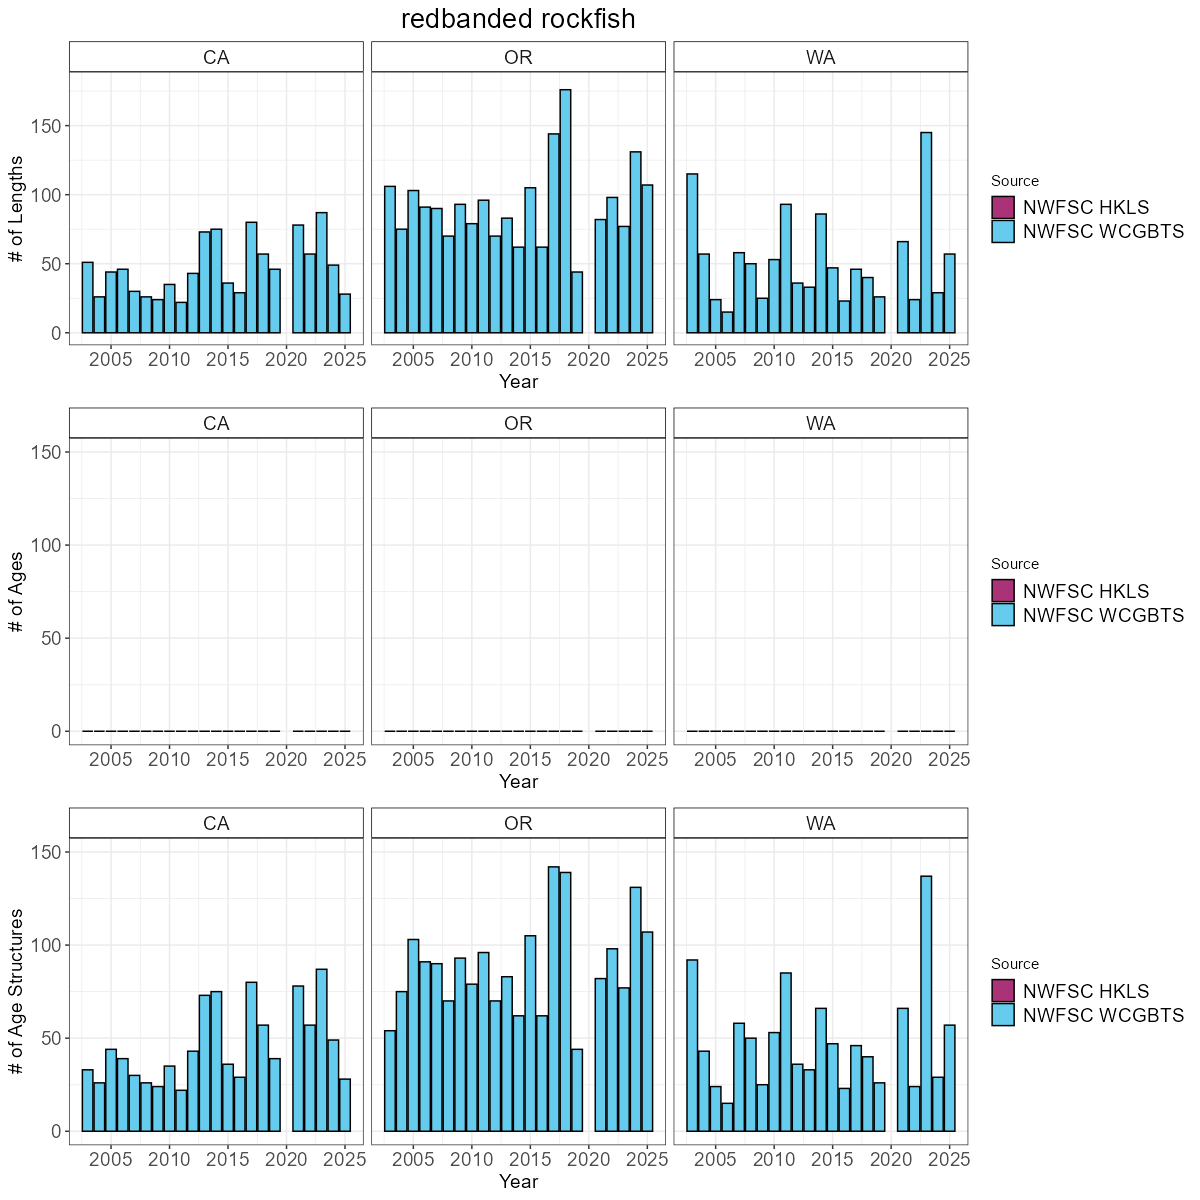
\includegraphics[keepaspectratio]{../plots/state_comparisons/redbanded_rockfish_state_compositions.png}}

}

\caption{Total number of available lengths, read ages, and unread age
structures by data source by year. Note the y-axis is unique for the
number of lengths plot row compared to the number of age and age
structure plot rows.}

\end{figure}%

\newpage{}

\subsection{Redstripe rockfish}\label{redstripe-rockfish}

To date, no assessment or analysis has been conducted on redstripe
rockfish. Across available data, redstripe rockfish have been observed
and sampled by the NWFSC WCGBT survey. The NWFSC WCGBTS survey has an
average of 12 positive tows per year. Across the coast a total of 0
maturity samples have been collected with 0 read maturities.

\begingroup\fontsize{10}{12}\selectfont
\begingroup\fontsize{10}{12}\selectfont

\begin{longtable}[t]{>{\raggedleft\arraybackslash}p{2cm}>{\raggedleft\arraybackslash}p{3.5cm}>{\raggedleft\arraybackslash}p{2cm}>{\raggedleft\arraybackslash}p{2cm}>{\raggedleft\arraybackslash}p{2cm}}
\caption{\label{tab:unnamed-chunk-141}Total number of available lengths, read ages, and unread age structures by data source and
state between for redstripe rockfish.}\\
\toprule
State & Source & Lengths & Ages & Age Structures\\
\midrule
\endfirsthead
\caption[]{Total number of available lengths, read ages, and unread age structures by data source and
state between for redstripe rockfish. (\textit{continued)}}\\
\toprule
State & Source & Lengths & Ages & Age Structures\\
\midrule
\endhead

\endfoot
\bottomrule
\endlastfoot
CA & NWFSC WCGBTS & 348 & 0 & 199\\
OR & NWFSC WCGBTS & 4,195 & 0 & 1,892\\
WA & NWFSC WCGBTS & 3,276 & 0 & 1,646\\*
\end{longtable}
\endgroup{}
\endgroup{}

\begin{figure}[H]

{\centering \pandocbounded{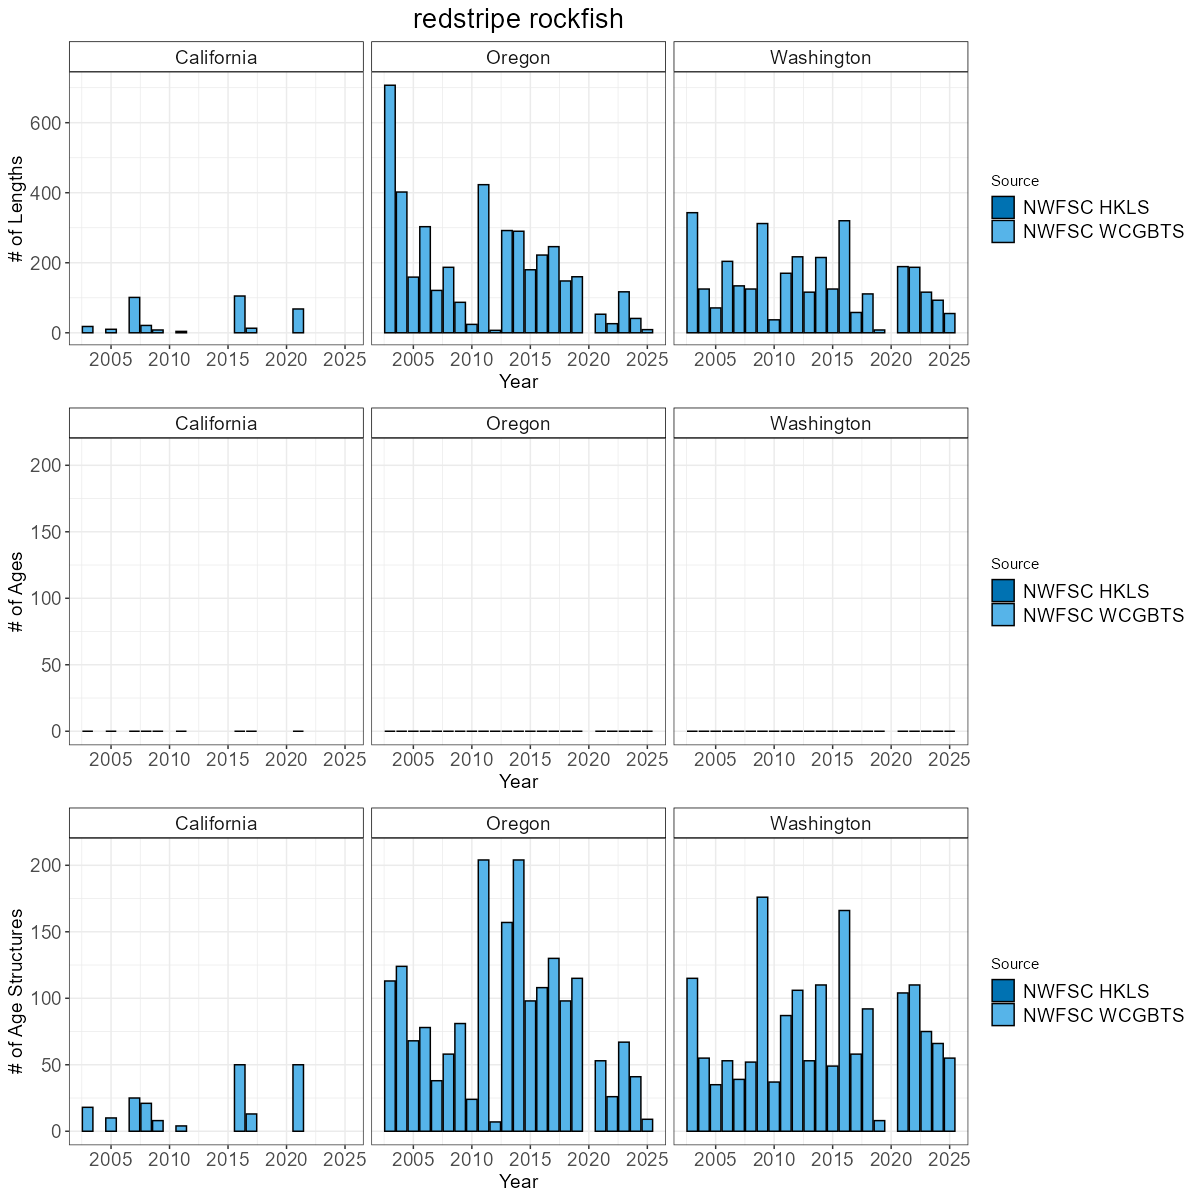
\includegraphics[keepaspectratio]{../plots/state_comparisons/redstripe_rockfish_state_compositions.png}}

}

\caption{Total number of available lengths, read ages, and unread age
structures by data source by year. Note the y-axis is unique for the
number of lengths plot row compared to the number of age and age
structure plot rows.}

\end{figure}%

\newpage{}

\subsection{Rex sole}\label{rex-sole}

The most recent assessment of rex sole was a data-moderate assessment
conducted in 2023. Across available data, rex sole have been observed
and sampled by the NWFSC WCGBT survey. The NWFSC WCGBTS survey has an
average of 367 positive tows per year. Across the coast a total of 0
maturity samples have been collected with 0 read maturities.

\begingroup\fontsize{10}{12}\selectfont
\begingroup\fontsize{10}{12}\selectfont

\begin{longtable}[t]{>{\raggedleft\arraybackslash}p{2cm}>{\raggedleft\arraybackslash}p{3.5cm}>{\raggedleft\arraybackslash}p{2cm}>{\raggedleft\arraybackslash}p{2cm}>{\raggedleft\arraybackslash}p{2cm}}
\caption{\label{tab:unnamed-chunk-146}Total number of available lengths, read ages, and unread age structures by data source and
state between for rex sole.}\\
\toprule
State & Source & Lengths & Ages & Age Structures\\
\midrule
\endfirsthead
\caption[]{Total number of available lengths, read ages, and unread age structures by data source and
state between for rex sole. (\textit{continued)}}\\
\toprule
State & Source & Lengths & Ages & Age Structures\\
\midrule
\endhead

\endfoot
\bottomrule
\endlastfoot
CA & NWFSC WCGBTS & 57,526 & 273 & 4,920\\
OR & NWFSC WCGBTS & 67,944 & 208 & 4,700\\
WA & NWFSC WCGBTS & 25,156 & 140 & 1,917\\*
\end{longtable}
\endgroup{}
\endgroup{}

\begin{figure}[H]

{\centering \pandocbounded{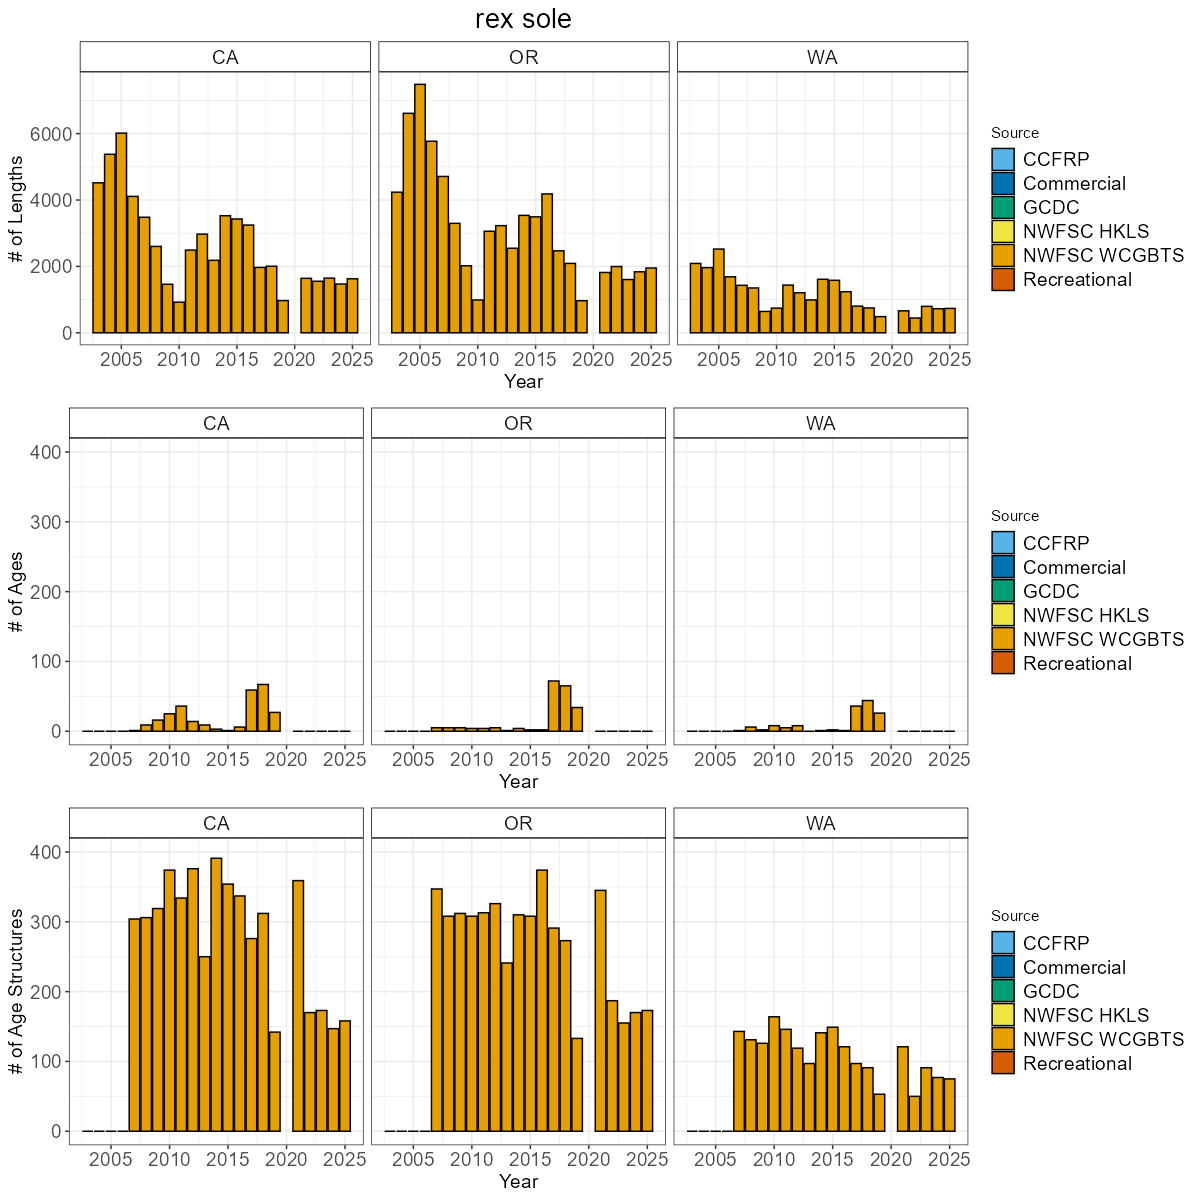
\includegraphics[keepaspectratio]{../plots/state_comparisons/rex_sole_state_compositions.png}}

}

\caption{Total number of available lengths, read ages, and unread age
structures by data source by year. Note the y-axis is unique for the
number of lengths plot row compared to the number of age and age
structure plot rows.}

\end{figure}%

\newpage{}

\subsection{Rosethorn rockfish}\label{rosethorn-rockfish}

To date, no assessment or analysis has been conducted on rosethorn
rockfish. Across available data, rosethorn rockfish have been observed
and sampled by the NWFSC WCGBT survey. The NWFSC WCGBTS survey has an
average of 46 positive tows per year. Across the coast a total of 0
maturity samples have been collected with 0 read maturities.

\begingroup\fontsize{10}{12}\selectfont
\begingroup\fontsize{10}{12}\selectfont

\begin{longtable}[t]{>{\raggedleft\arraybackslash}p{2cm}>{\raggedleft\arraybackslash}p{3.5cm}>{\raggedleft\arraybackslash}p{2cm}>{\raggedleft\arraybackslash}p{2cm}>{\raggedleft\arraybackslash}p{2cm}}
\caption{\label{tab:unnamed-chunk-151}Total number of available lengths, read ages, and unread age structures by data source and
state between for rosethorn rockfish.}\\
\toprule
State & Source & Lengths & Ages & Age Structures\\
\midrule
\endfirsthead
\caption[]{Total number of available lengths, read ages, and unread age structures by data source and
state between for rosethorn rockfish. (\textit{continued)}}\\
\toprule
State & Source & Lengths & Ages & Age Structures\\
\midrule
\endhead

\endfoot
\bottomrule
\endlastfoot
CA & NWFSC HKL & 36 & 0 & 27\\
CA & NWFSC WCGBTS & 3,060 & 0 & 1,528\\
OR & NWFSC WCGBTS & 10,290 & 0 & 4,214\\
WA & NWFSC WCGBTS & 6,822 & 0 & 2,827\\*
\end{longtable}
\endgroup{}
\endgroup{}

\begin{figure}[H]

{\centering \pandocbounded{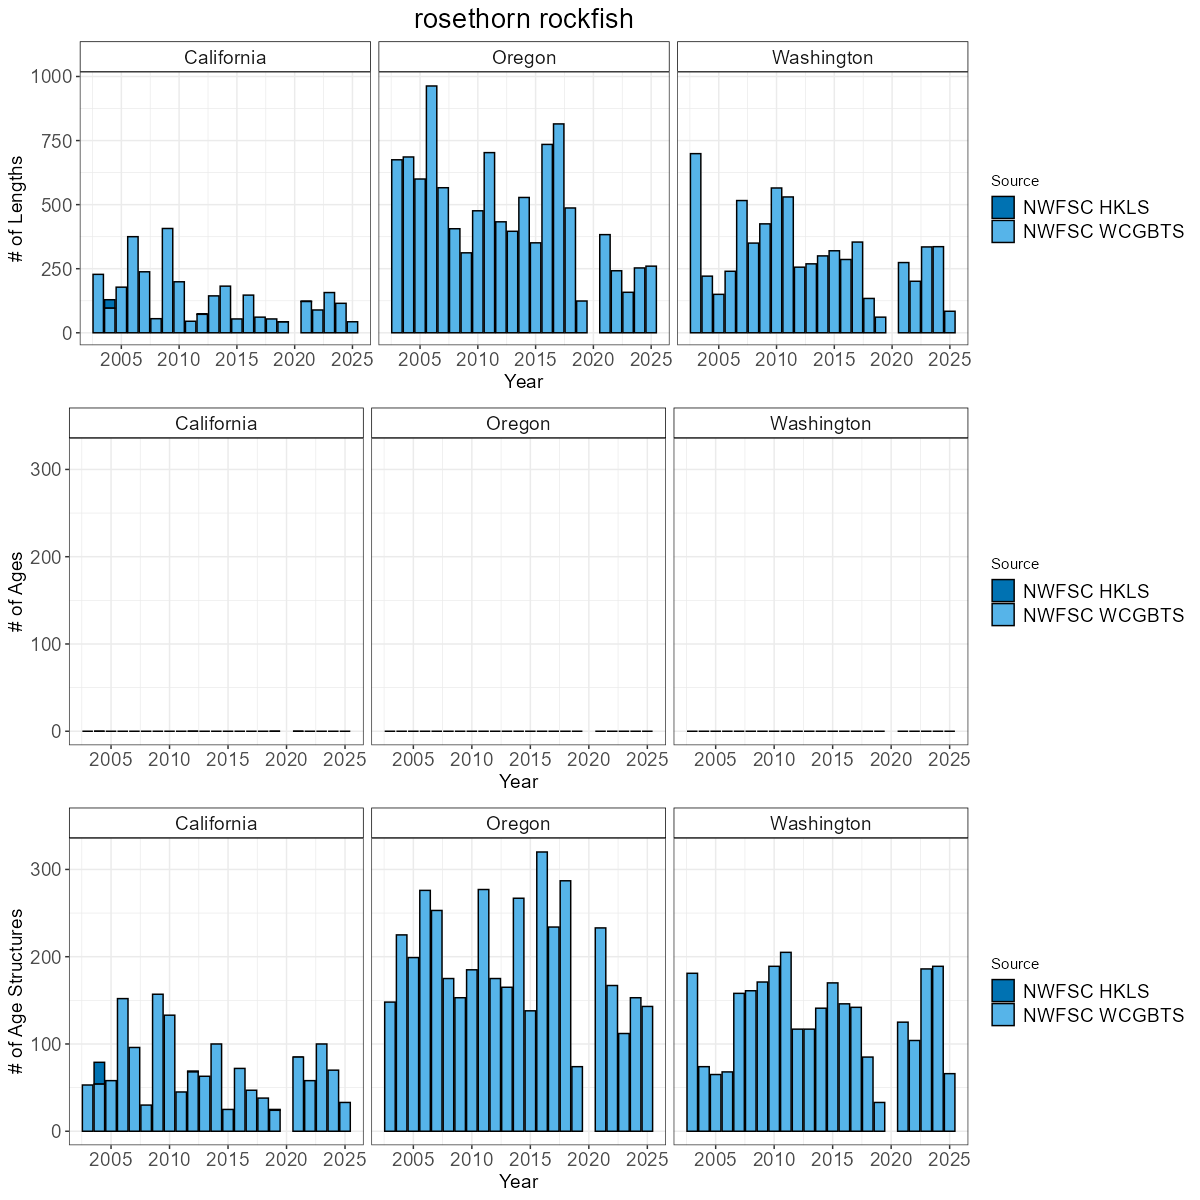
\includegraphics[keepaspectratio]{../plots/state_comparisons/rosethorn_rockfish_state_compositions.png}}

}

\caption{Total number of available lengths, read ages, and unread age
structures by data source by year. Note the y-axis is unique for the
number of lengths plot row compared to the number of age and age
structure plot rows.}

\end{figure}%

\newpage{}

\subsection{Rougheye and blackspotted
rockfish}\label{rougheye-and-blackspotted-rockfish}

The most recent assessment of rougheye and blackspotted rockfish was a
benchmark assessment conducted in 2025. Across available data, rougheye
and blackspotted rockfish have been observed and sampled by the NWFSC
WCGBT survey. The NWFSC WCGBTS survey has an average of 27 positive tows
per year. Across the coast a total of 549 maturity samples have been
collected with 549 read maturities.

\begingroup\fontsize{10}{12}\selectfont
\begingroup\fontsize{10}{12}\selectfont

\begin{longtable}[t]{>{\raggedleft\arraybackslash}p{2cm}>{\raggedleft\arraybackslash}p{3.5cm}>{\raggedleft\arraybackslash}p{2cm}>{\raggedleft\arraybackslash}p{2cm}>{\raggedleft\arraybackslash}p{2cm}}
\caption{\label{tab:unnamed-chunk-156}Total number of available lengths, read ages, and unread age structures by data source and
state between for rougheye and blackspotted rockfish.}\\
\toprule
State & Source & Lengths & Ages & Age Structures\\
\midrule
\endfirsthead
\caption[]{Total number of available lengths, read ages, and unread age structures by data source and
state between for rougheye and blackspotted rockfish. (\textit{continued)}}\\
\toprule
State & Source & Lengths & Ages & Age Structures\\
\midrule
\endhead

\endfoot
\bottomrule
\endlastfoot
CA & NWFSC HKL & 1 & 0 & 1\\
CA & NWFSC WCGBTS & 15 & 14 & 0\\
OR & NWFSC WCGBTS & 1,104 & 919 & 13\\
WA & NWFSC WCGBTS & 1,182 & 1,029 & 3\\*
\end{longtable}
\endgroup{}
\endgroup{}

\begin{figure}[H]

{\centering \pandocbounded{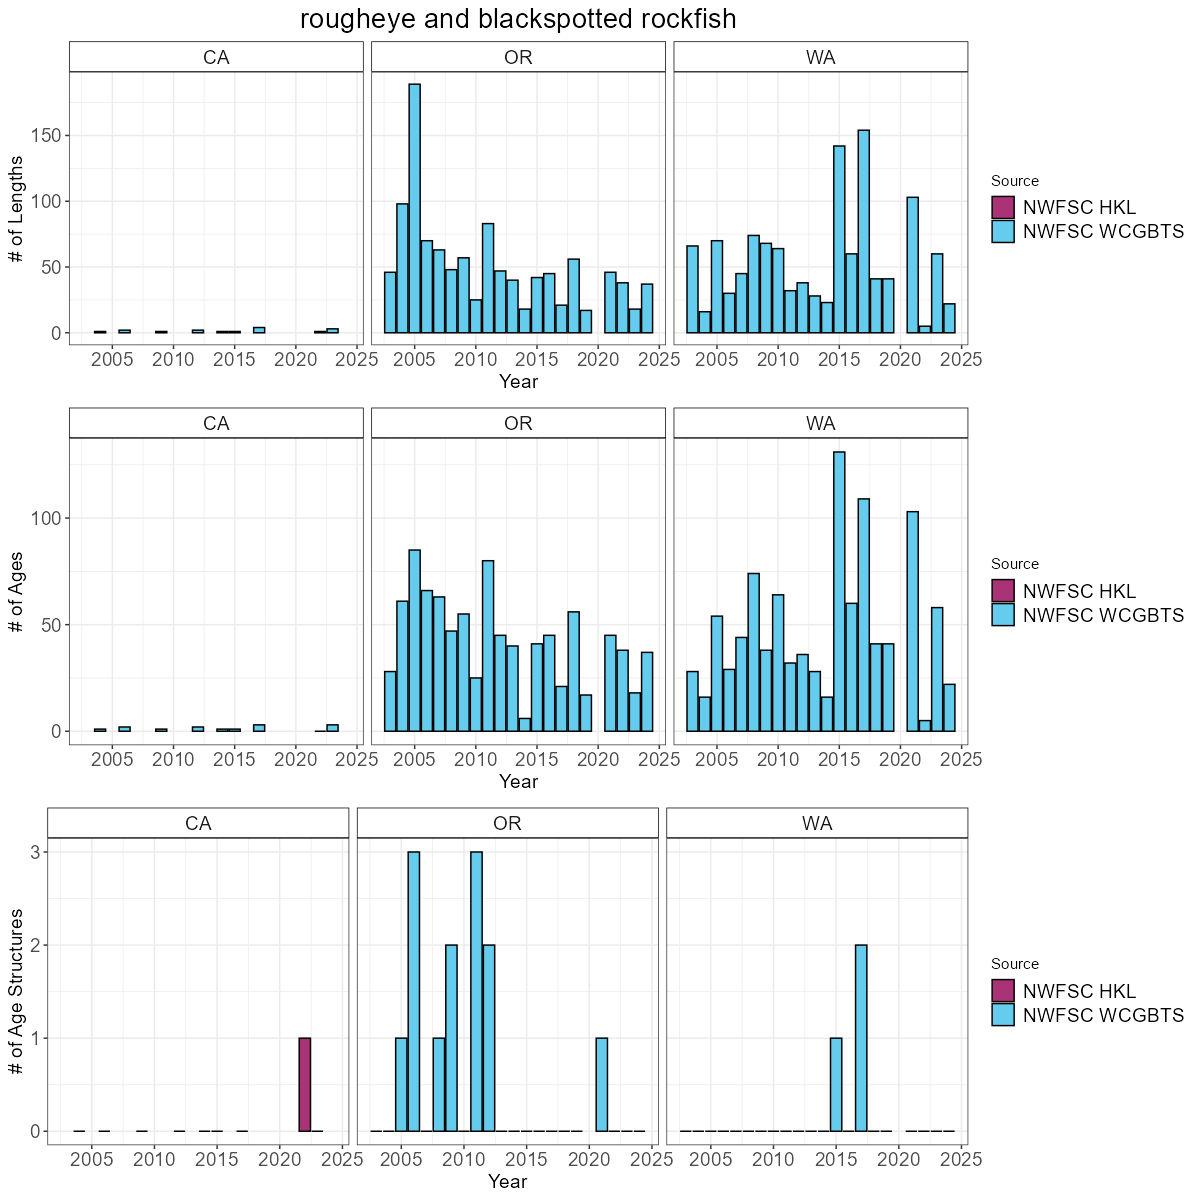
\includegraphics[keepaspectratio]{../plots/state_comparisons/rougheye_and_blackspotted_rockfish_state_compositions.png}}

}

\caption{Total number of available lengths, read ages, and unread age
structures by data source by year. Note the y-axis is unique for the
number of lengths plot row compared to the number of age and age
structure plot rows.}

\end{figure}%

\newpage{}

\subsection{Sablefish}\label{sablefish}

The most recent assessment of sablefish was a benchmark assessment
conducted in 2025. Across available data, sablefish have been observed
and sampled by the NWFSC WCGBT survey. The NWFSC WCGBTS survey has an
average of 404 positive tows per year. Across the coast a total of 1312
maturity samples have been collected with 1157 read maturities.

\begingroup\fontsize{10}{12}\selectfont
\begingroup\fontsize{10}{12}\selectfont

\begin{longtable}[t]{>{\raggedleft\arraybackslash}p{2cm}>{\raggedleft\arraybackslash}p{3.5cm}>{\raggedleft\arraybackslash}p{2cm}>{\raggedleft\arraybackslash}p{2cm}>{\raggedleft\arraybackslash}p{2cm}}
\caption{\label{tab:unnamed-chunk-161}Total number of available lengths, read ages, and unread age structures by data source and
state between for sablefish.}\\
\toprule
State & Source & Lengths & Ages & Age Structures\\
\midrule
\endfirsthead
\caption[]{Total number of available lengths, read ages, and unread age structures by data source and
state between for sablefish. (\textit{continued)}}\\
\toprule
State & Source & Lengths & Ages & Age Structures\\
\midrule
\endhead

\endfoot
\bottomrule
\endlastfoot
CA & NWFSC WCGBTS & 50,794 & 13,641 & 6,031\\
OR & NWFSC WCGBTS & 36,899 & 9,952 & 4,228\\
WA & NWFSC WCGBTS & 13,340 & 3,931 & 1,537\\*
\end{longtable}
\endgroup{}
\endgroup{}

\begin{figure}[H]

{\centering \pandocbounded{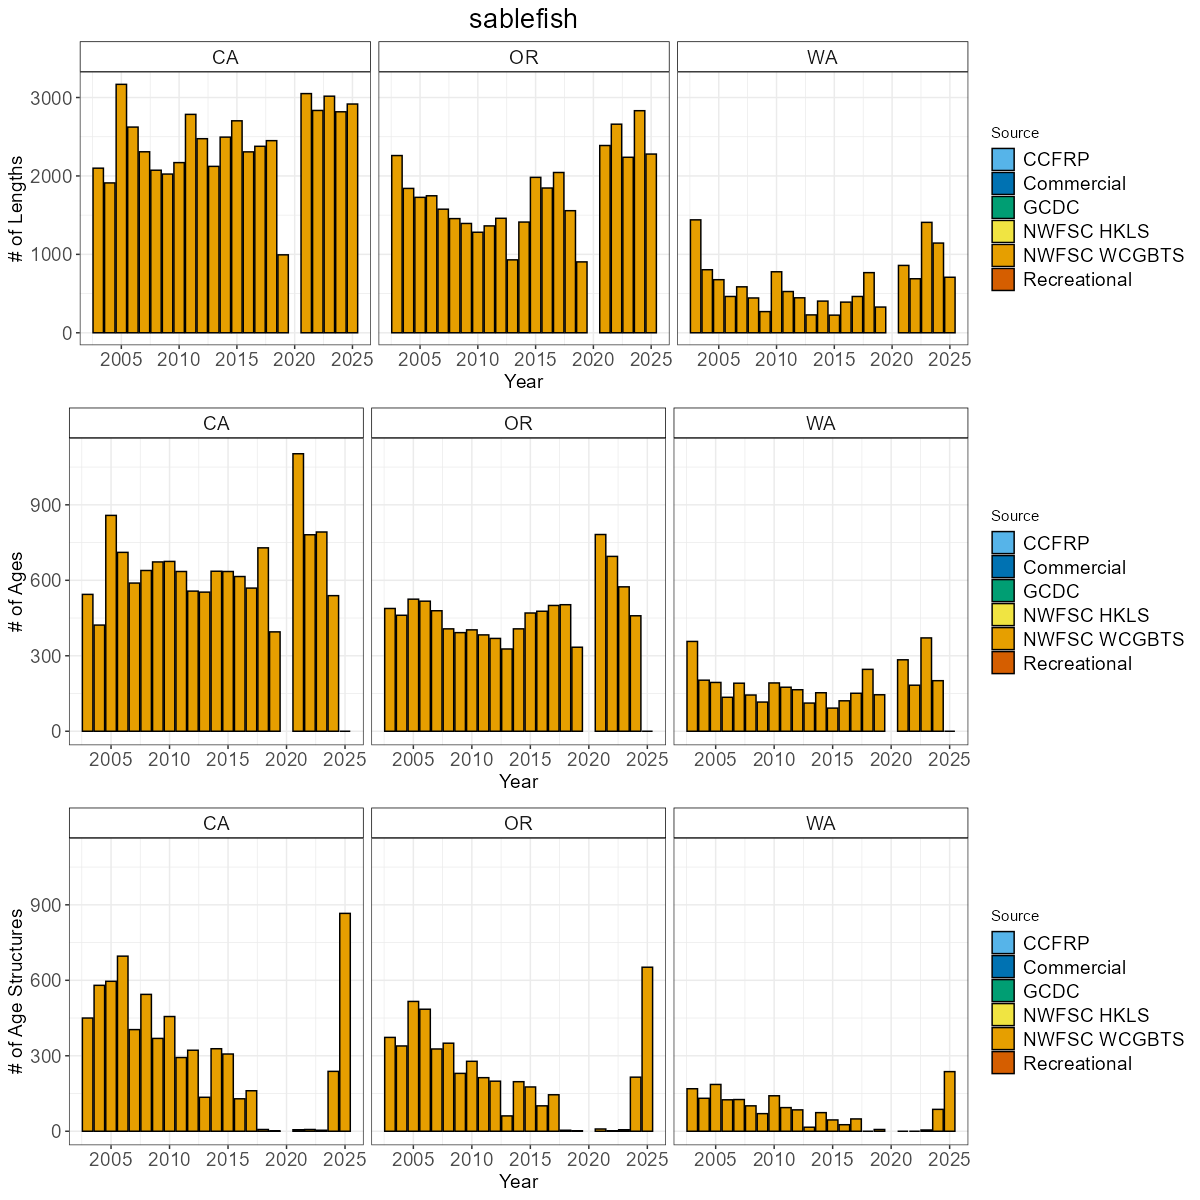
\includegraphics[keepaspectratio]{../plots/state_comparisons/sablefish_state_compositions.png}}

}

\caption{Total number of available lengths, read ages, and unread age
structures by data source by year. Note the y-axis is unique for the
number of lengths plot row compared to the number of age and age
structure plot rows.}

\end{figure}%

\newpage{}

\subsection{Sharpchin rockfish}\label{sharpchin-rockfish}

The most recent assessment of sharpchin rockfish was a data-moderate
assessment conducted in 2013. Across available data, sharpchin rockfish
have been observed and sampled by the NWFSC WCGBT survey. The NWFSC
WCGBTS survey has an average of 41 positive tows per year. Across the
coast a total of 0 maturity samples have been collected with 0 read
maturities.

\begingroup\fontsize{10}{12}\selectfont
\begingroup\fontsize{10}{12}\selectfont

\begin{longtable}[t]{>{\raggedleft\arraybackslash}p{2cm}>{\raggedleft\arraybackslash}p{3.5cm}>{\raggedleft\arraybackslash}p{2cm}>{\raggedleft\arraybackslash}p{2cm}>{\raggedleft\arraybackslash}p{2cm}}
\caption{\label{tab:unnamed-chunk-166}Total number of available lengths, read ages, and unread age structures by data source and
state between for sharpchin rockfish.}\\
\toprule
State & Source & Lengths & Ages & Age Structures\\
\midrule
\endfirsthead
\caption[]{Total number of available lengths, read ages, and unread age structures by data source and
state between for sharpchin rockfish. (\textit{continued)}}\\
\toprule
State & Source & Lengths & Ages & Age Structures\\
\midrule
\endhead

\endfoot
\bottomrule
\endlastfoot
CA & NWFSC HKL & 13 & 0 & 13\\
CA & NWFSC WCGBTS & 3,704 & 0 & 1,874\\
OR & NWFSC WCGBTS & 10,182 & 0 & 4,153\\
WA & NWFSC WCGBTS & 6,869 & 0 & 3,072\\*
\end{longtable}
\endgroup{}
\endgroup{}

\begin{figure}[H]

{\centering \pandocbounded{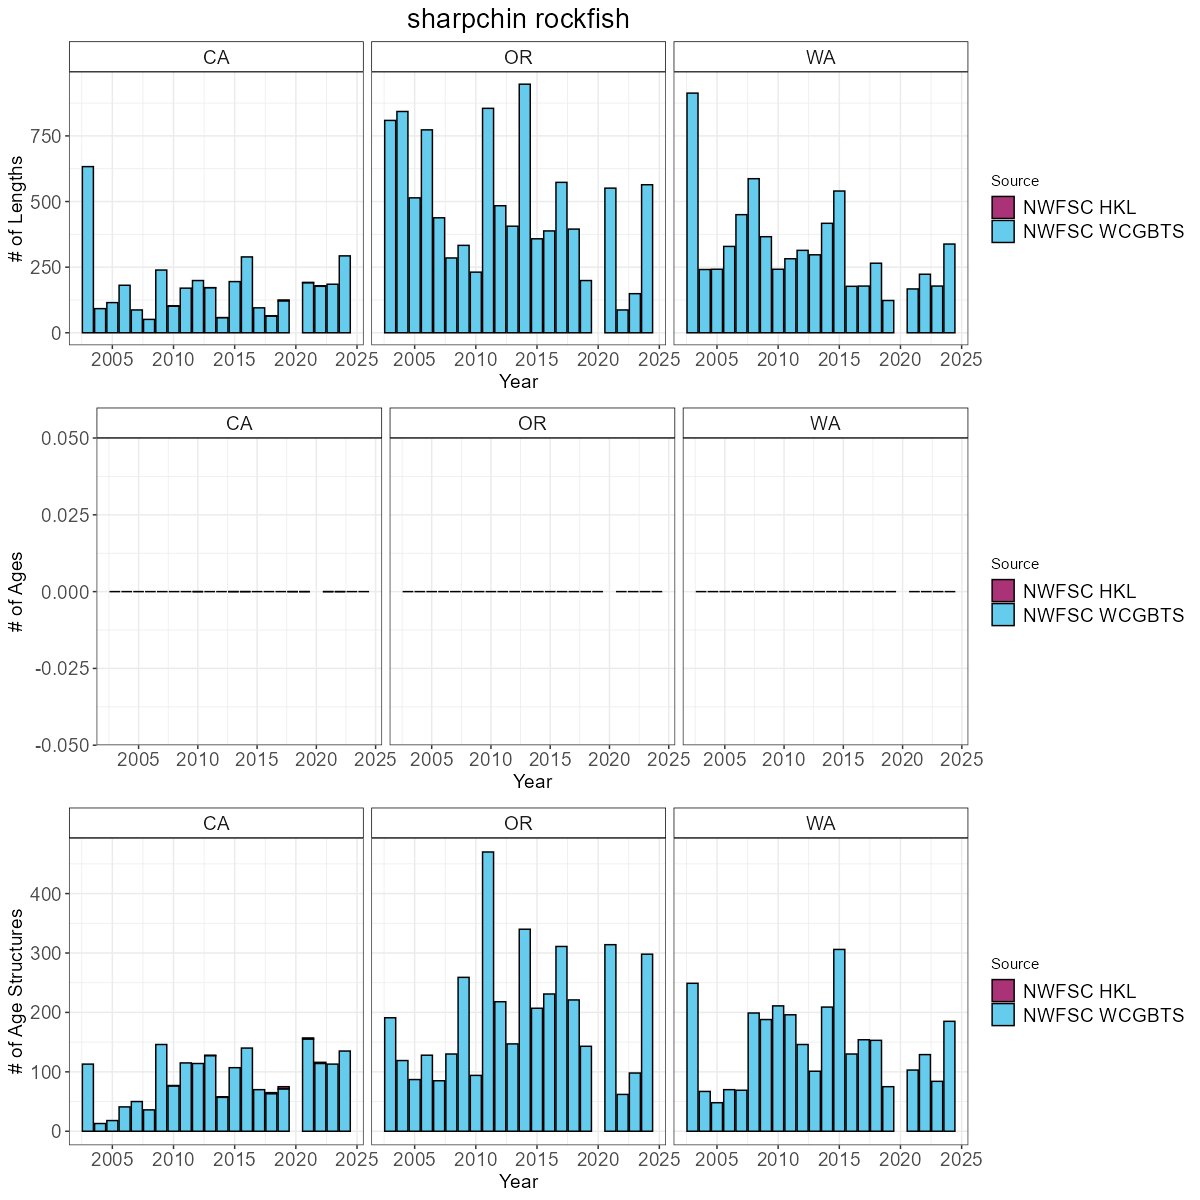
\includegraphics[keepaspectratio]{../plots/state_comparisons/sharpchin_rockfish_state_compositions.png}}

}

\caption{Total number of available lengths, read ages, and unread age
structures by data source by year. Note the y-axis is unique for the
number of lengths plot row compared to the number of age and age
structure plot rows.}

\end{figure}%

\newpage{}

\subsection{Shortspine thornyhead}\label{shortspine-thornyhead}

The most recent assessment of shortspine thornyhead was a data-moderate
assessment conducted in 2023. Across available data, shortspine
thornyhead have been observed and sampled by the NWFSC WCGBT survey. The
NWFSC WCGBTS survey has an average of 308 positive tows per year. Across
the coast a total of 1136 maturity samples have been collected with 862
read maturities.

\begingroup\fontsize{10}{12}\selectfont
\begingroup\fontsize{10}{12}\selectfont

\begin{longtable}[t]{>{\raggedleft\arraybackslash}p{2cm}>{\raggedleft\arraybackslash}p{3.5cm}>{\raggedleft\arraybackslash}p{2cm}>{\raggedleft\arraybackslash}p{2cm}>{\raggedleft\arraybackslash}p{2cm}}
\caption{\label{tab:unnamed-chunk-172}Total number of available lengths, read ages, and unread age structures by data source and
state between for shortspine thornyhead.}\\
\toprule
State & Source & Lengths & Ages & Age Structures\\
\midrule
\endfirsthead
\caption[]{Total number of available lengths, read ages, and unread age structures by data source and
state between for shortspine thornyhead. (\textit{continued)}}\\
\toprule
State & Source & Lengths & Ages & Age Structures\\
\midrule
\endhead

\endfoot
\bottomrule
\endlastfoot
CA & NWFSC WCGBTS & 48,129 & 0 & 12,092\\
OR & NWFSC WCGBTS & 42,573 & 0 & 7,321\\
WA & NWFSC WCGBTS & 12,585 & 0 & 2,724\\*
\end{longtable}
\endgroup{}
\endgroup{}

\begin{figure}[H]

{\centering \pandocbounded{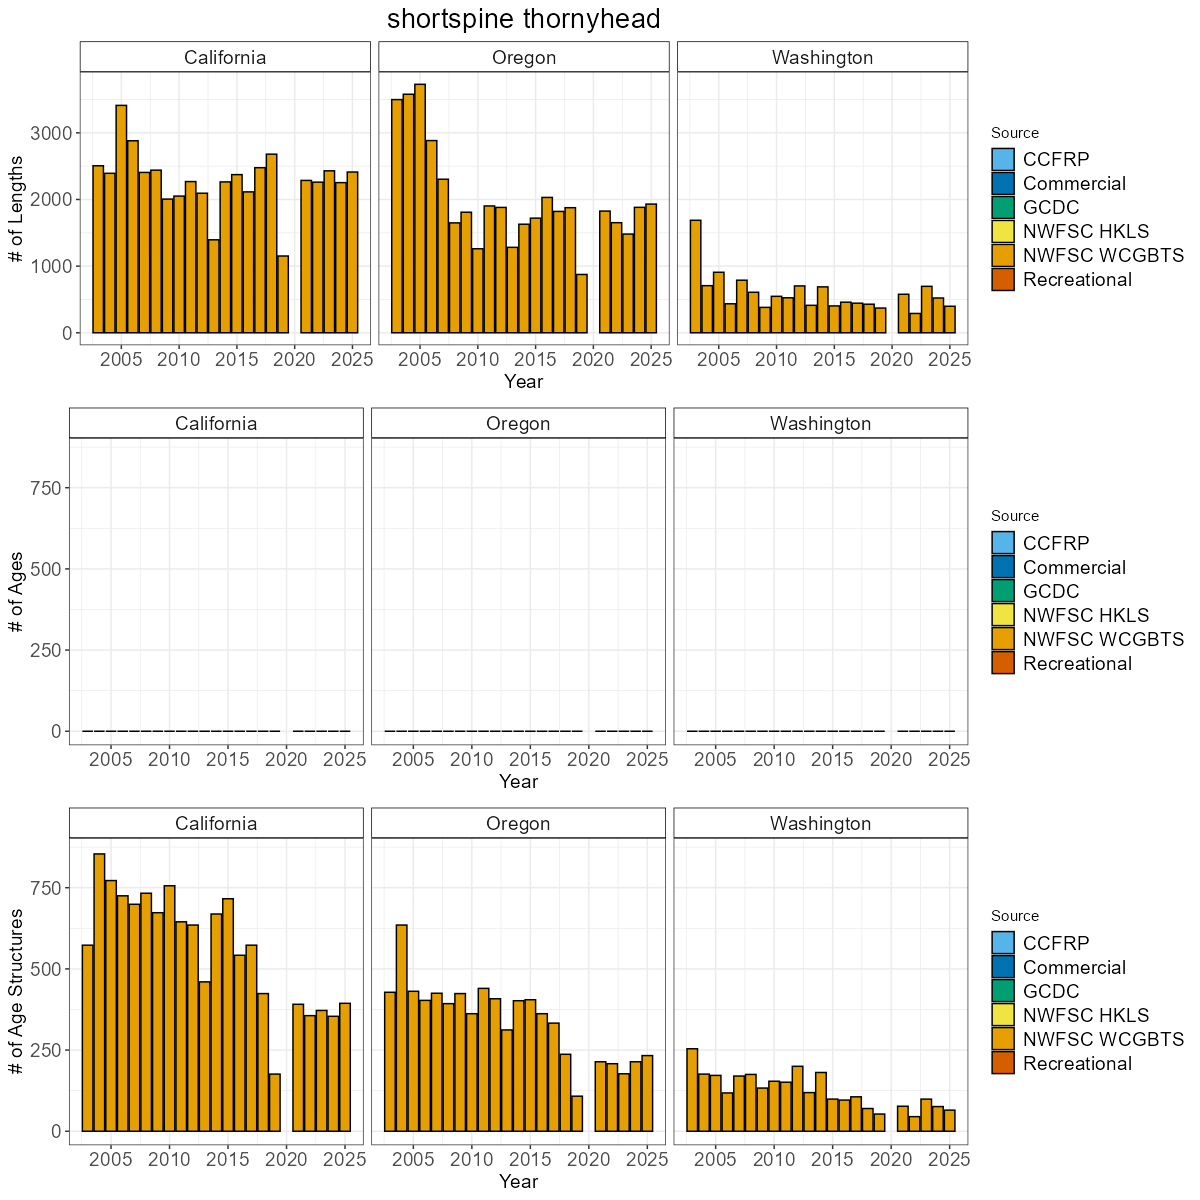
\includegraphics[keepaspectratio]{../plots/state_comparisons/shortspine_thornyhead_state_compositions.png}}

}

\caption{Total number of available lengths, read ages, and unread age
structures by data source by year. Note the y-axis is unique for the
number of lengths plot row compared to the number of age and age
structure plot rows.}

\end{figure}%

\newpage{}

\subsection{Silvergray rockfish}\label{silvergray-rockfish}

To date, no assessment or analysis has been conducted on silvergray
rockfish. Across available data, silvergray rockfish have been observed
and sampled by the NWFSC WCGBT survey. The NWFSC WCGBTS survey has an
average of 6 positive tows per year. Across the coast a total of 0
maturity samples have been collected with 0 read maturities.

\begingroup\fontsize{10}{12}\selectfont
\begingroup\fontsize{10}{12}\selectfont

\begin{longtable}[t]{>{\raggedleft\arraybackslash}p{2cm}>{\raggedleft\arraybackslash}p{3.5cm}>{\raggedleft\arraybackslash}p{2cm}>{\raggedleft\arraybackslash}p{2cm}>{\raggedleft\arraybackslash}p{2cm}}
\caption{\label{tab:unnamed-chunk-177}Total number of available lengths, read ages, and unread age structures by data source and
state between for silvergray rockfish.}\\
\toprule
State & Source & Lengths & Ages & Age Structures\\
\midrule
\endfirsthead
\caption[]{Total number of available lengths, read ages, and unread age structures by data source and
state between for silvergray rockfish. (\textit{continued)}}\\
\toprule
State & Source & Lengths & Ages & Age Structures\\
\midrule
\endhead

\endfoot
\bottomrule
\endlastfoot
CA & NWFSC HKL & 4 & 0 & 3\\
CA & NWFSC WCGBTS & 15 & 0 & 15\\
OR & NWFSC WCGBTS & 481 & 0 & 393\\
WA & NWFSC WCGBTS & 425 & 0 & 398\\*
\end{longtable}
\endgroup{}
\endgroup{}

\begin{figure}[H]

{\centering \pandocbounded{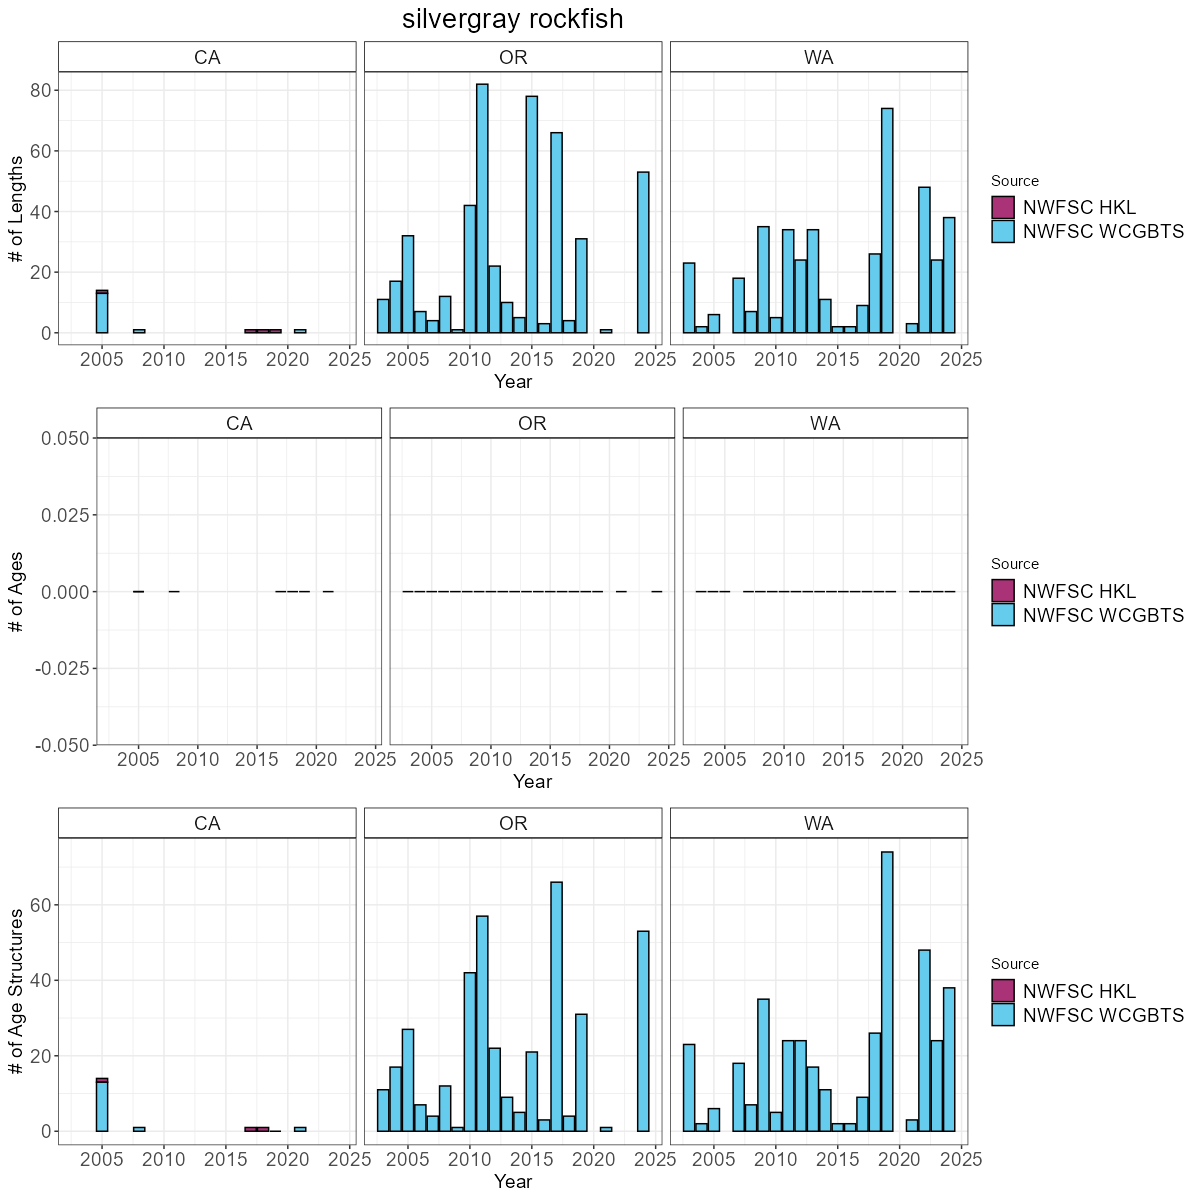
\includegraphics[keepaspectratio]{../plots/state_comparisons/silvergray_rockfish_state_compositions.png}}

}

\caption{Total number of available lengths, read ages, and unread age
structures by data source by year. Note the y-axis is unique for the
number of lengths plot row compared to the number of age and age
structure plot rows.}

\end{figure}%

\newpage{}

\subsection{Splitnose rockfish}\label{splitnose-rockfish}

The most recent assessment of splitnose rockfish was a benchmark
assessment conducted in 2009. Across available data, splitnose rockfish
have been observed and sampled by the NWFSC WCGBT survey. The NWFSC
WCGBTS survey has an average of 122 positive tows per year. Across the
coast a total of 0 maturity samples have been collected with 0 read
maturities.

\begingroup\fontsize{10}{12}\selectfont
\begingroup\fontsize{10}{12}\selectfont

\begin{longtable}[t]{>{\raggedleft\arraybackslash}p{2cm}>{\raggedleft\arraybackslash}p{3.5cm}>{\raggedleft\arraybackslash}p{2cm}>{\raggedleft\arraybackslash}p{2cm}>{\raggedleft\arraybackslash}p{2cm}}
\caption{\label{tab:unnamed-chunk-182}Total number of available lengths, read ages, and unread age structures by data source and
state between for splitnose rockfish.}\\
\toprule
State & Source & Lengths & Ages & Age Structures\\
\midrule
\endfirsthead
\caption[]{Total number of available lengths, read ages, and unread age structures by data source and
state between for splitnose rockfish. (\textit{continued)}}\\
\toprule
State & Source & Lengths & Ages & Age Structures\\
\midrule
\endhead

\endfoot
\bottomrule
\endlastfoot
CA & NWFSC WCGBTS & 33,681 & 1,573 & 6,123\\
OR & NWFSC WCGBTS & 17,858 & 1,044 & 3,584\\
WA & NWFSC WCGBTS & 3,145 & 294 & 654\\*
\end{longtable}
\endgroup{}
\endgroup{}

\begin{figure}[H]

{\centering \pandocbounded{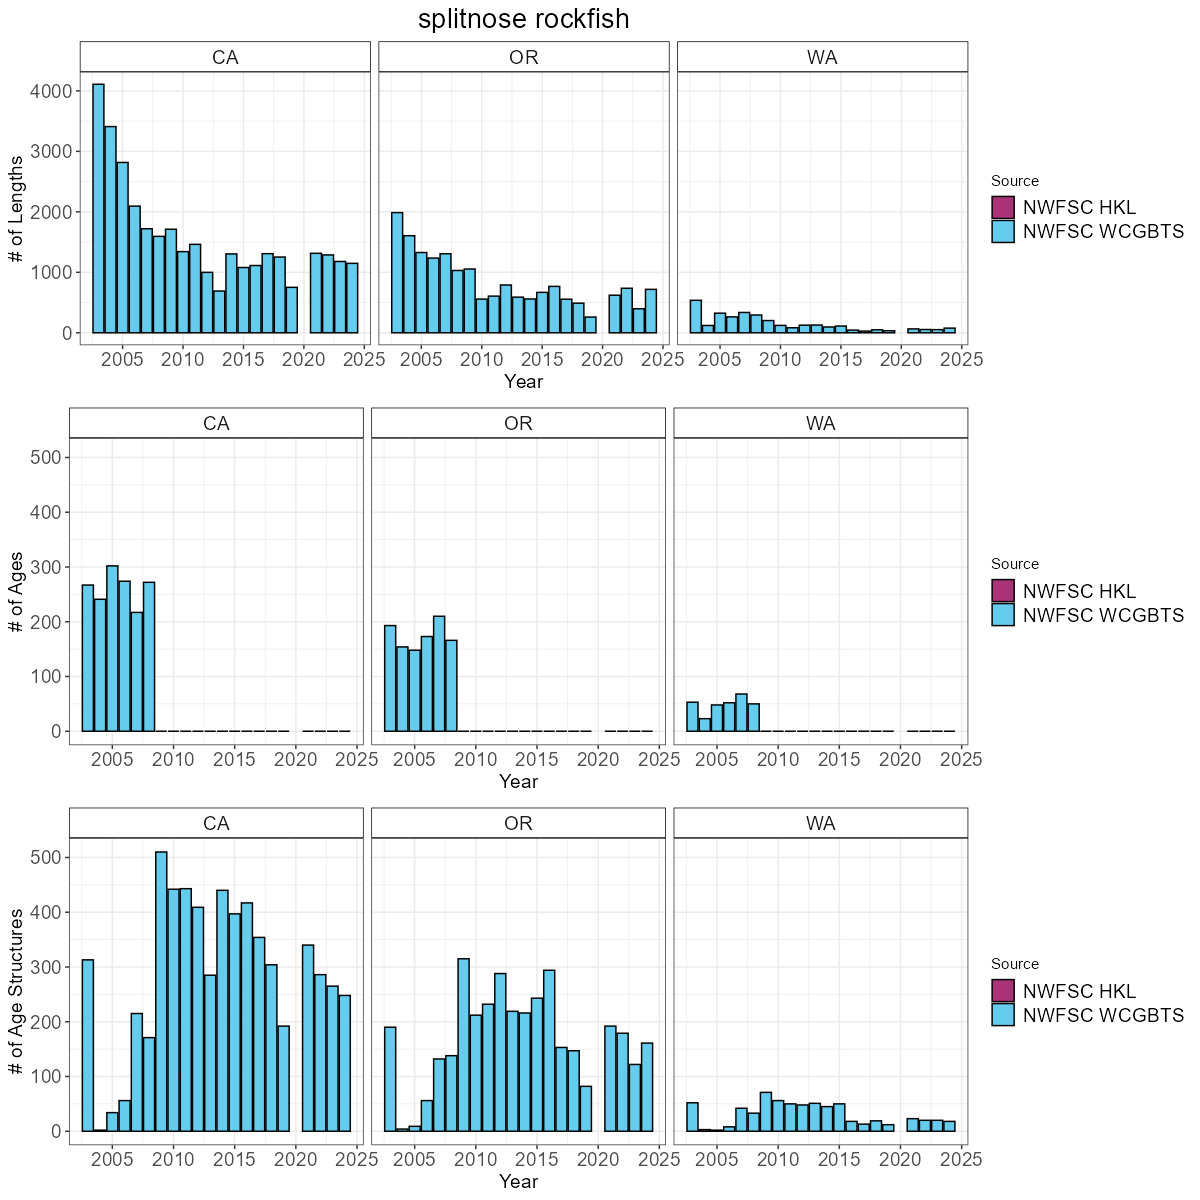
\includegraphics[keepaspectratio]{../plots/state_comparisons/splitnose_rockfish_state_compositions.png}}

}

\caption{Total number of available lengths, read ages, and unread age
structures by data source by year. Note the y-axis is unique for the
number of lengths plot row compared to the number of age and age
structure plot rows.}

\end{figure}%

\newpage{}

\subsection{Squarespot rockfish}\label{squarespot-rockfish}

The most recent assessment of squarespot rockfish was a data-moderate
assessment conducted in 2021. Across available data, squarespot rockfish
have been observed and sampled by both the NWFSC WCGBT and HKL surveys.
The NWFSC HKL survey has an average of 28 positive tows per year. The
NWFSC WCGBTS survey has an average of 9 positive tows per year. Across
the coast a total of 118 maturity samples have been collected with 118
read maturities.

\begingroup\fontsize{10}{12}\selectfont
\begingroup\fontsize{10}{12}\selectfont

\begin{longtable}[t]{>{\raggedleft\arraybackslash}p{2cm}>{\raggedleft\arraybackslash}p{3.5cm}>{\raggedleft\arraybackslash}p{2cm}>{\raggedleft\arraybackslash}p{2cm}>{\raggedleft\arraybackslash}p{2cm}}
\caption{\label{tab:unnamed-chunk-187}Total number of available lengths, read ages, and unread age structures by data source and
state between for squarespot rockfish.}\\
\toprule
State & Source & Lengths & Ages & Age Structures\\
\midrule
\endfirsthead
\caption[]{Total number of available lengths, read ages, and unread age structures by data source and
state between for squarespot rockfish. (\textit{continued)}}\\
\toprule
State & Source & Lengths & Ages & Age Structures\\
\midrule
\endhead

\endfoot
\bottomrule
\endlastfoot
CA & NWFSC HKL & 2,309 & 344 & 1,862\\
CA & NWFSC WCGBTS & 4,929 & 402 & 1,210\\
OR & NWFSC WCGBTS & 4 & 1 & 1\\*
\end{longtable}
\endgroup{}
\endgroup{}

\begin{figure}[H]

{\centering \pandocbounded{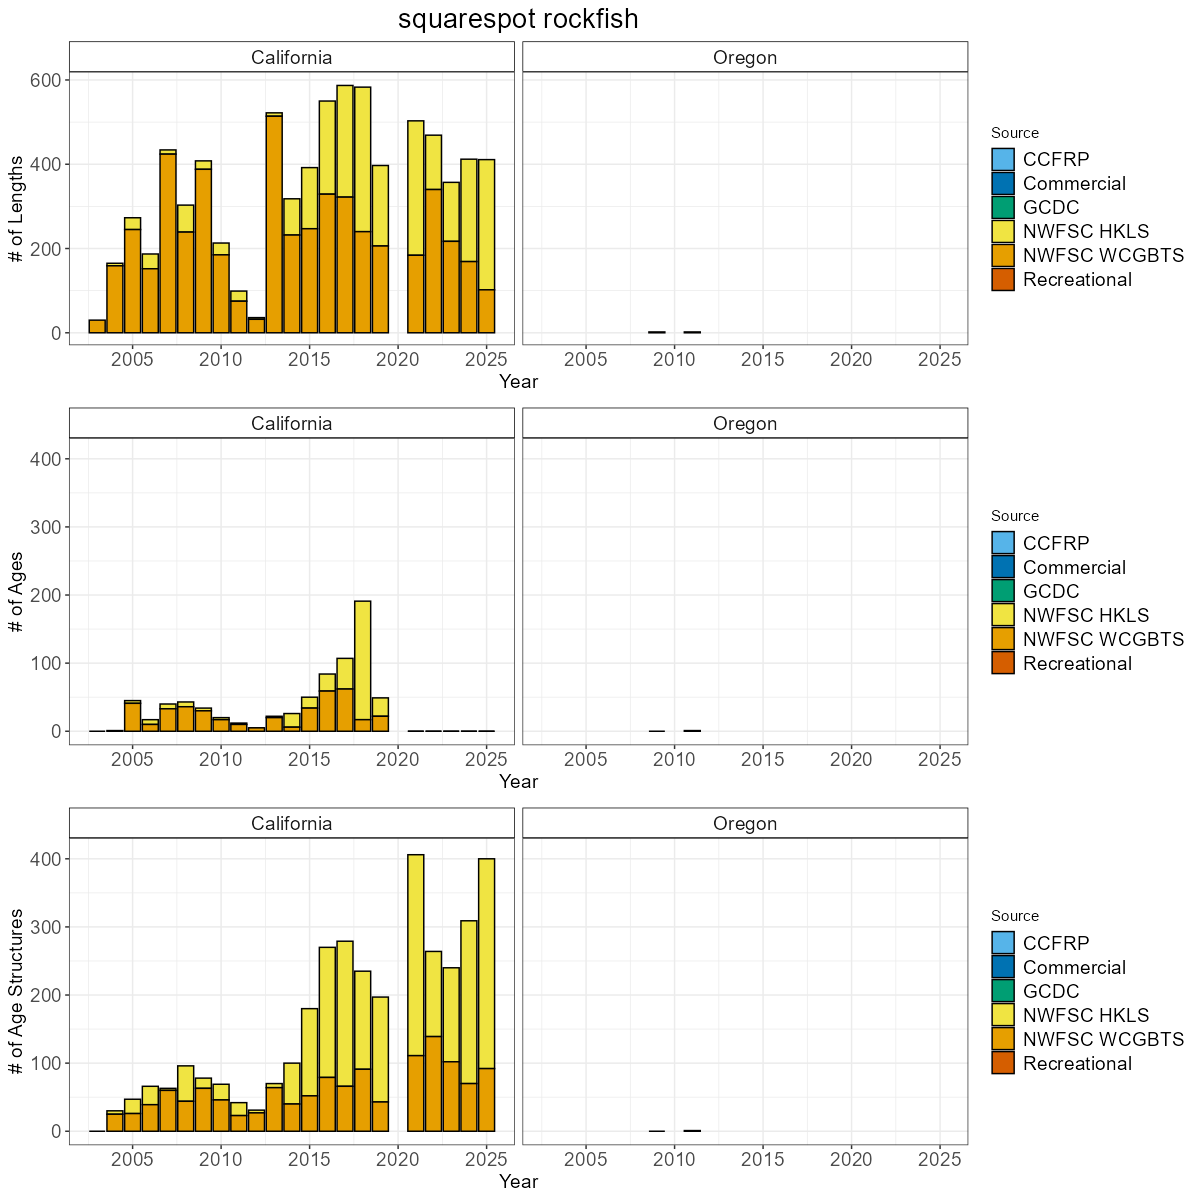
\includegraphics[keepaspectratio]{../plots/state_comparisons/squarespot_rockfish_state_compositions.png}}

}

\caption{Total number of available lengths, read ages, and unread age
structures by data source by year. Note the y-axis is unique for the
number of lengths plot row compared to the number of age and age
structure plot rows.}

\end{figure}%

\newpage{}

\subsection{Starry rockfish}\label{starry-rockfish}

To date, no assessment or analysis has been conducted on starry
rockfish. Across available data, starry rockfish have been observed and
sampled by the NWFSC HKL survey. The NWFSC HKL survey has an average of
52 positive tows per year. Across the coast a total of 340 maturity
samples have been collected with 0 read maturities.

\begingroup\fontsize{10}{12}\selectfont
\begingroup\fontsize{10}{12}\selectfont

\begin{longtable}[t]{>{\raggedleft\arraybackslash}p{2cm}>{\raggedleft\arraybackslash}p{3.5cm}>{\raggedleft\arraybackslash}p{2cm}>{\raggedleft\arraybackslash}p{2cm}>{\raggedleft\arraybackslash}p{2cm}}
\caption{\label{tab:unnamed-chunk-192}Total number of available lengths, read ages, and unread age structures by data source and
state between for starry rockfish.}\\
\toprule
State & Source & Lengths & Ages & Age Structures\\
\midrule
\endfirsthead
\caption[]{Total number of available lengths, read ages, and unread age structures by data source and
state between for starry rockfish. (\textit{continued)}}\\
\toprule
State & Source & Lengths & Ages & Age Structures\\
\midrule
\endhead

\endfoot
\bottomrule
\endlastfoot
CA & NWFSC HKL & 3,692 & 0 & 3,566\\
CA & NWFSC WCGBTS & 98 & 0 & 91\\*
\end{longtable}
\endgroup{}
\endgroup{}

\begin{figure}[H]

{\centering \pandocbounded{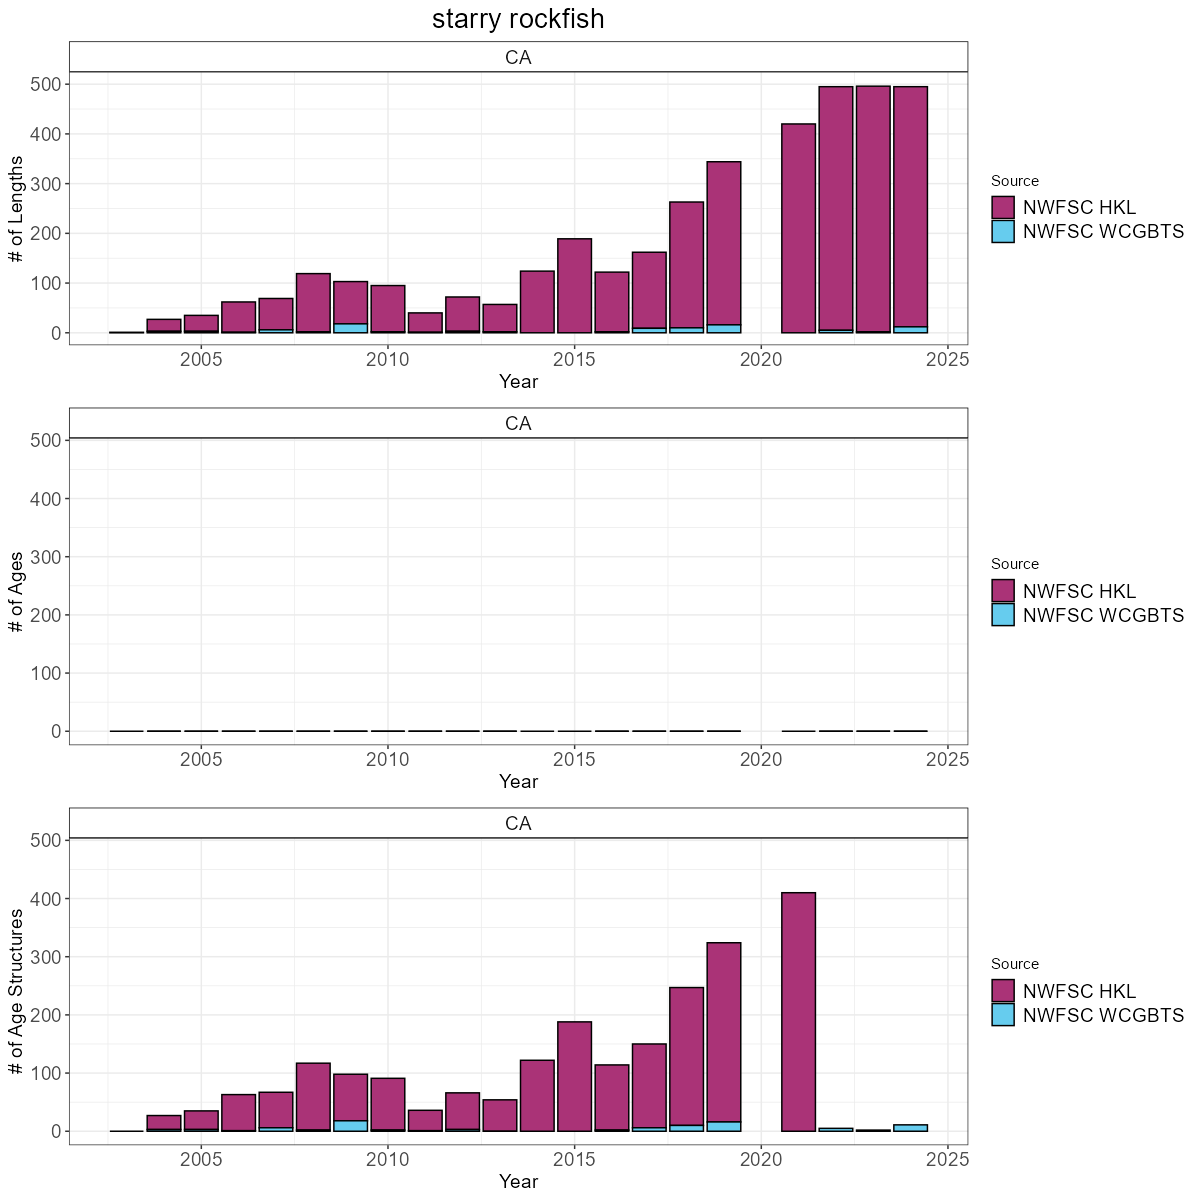
\includegraphics[keepaspectratio]{../plots/state_comparisons/starry_rockfish_state_compositions.png}}

}

\caption{Total number of available lengths, read ages, and unread age
structures by data source by year. Note the y-axis is unique for the
number of lengths plot row compared to the number of age and age
structure plot rows.}

\end{figure}%

\newpage{}

\subsection{Stripetail rockfish}\label{stripetail-rockfish}

To date, no assessment or analysis has been conducted on stripetail
rockfish. Across available data, stripetail rockfish have been observed
and sampled by the NWFSC WCGBT survey. The NWFSC WCGBTS survey has an
average of 133 positive tows per year. Across the coast a total of 67
maturity samples have been collected with 67 read maturities.

\begingroup\fontsize{10}{12}\selectfont
\begingroup\fontsize{10}{12}\selectfont

\begin{longtable}[t]{>{\raggedleft\arraybackslash}p{2cm}>{\raggedleft\arraybackslash}p{3.5cm}>{\raggedleft\arraybackslash}p{2cm}>{\raggedleft\arraybackslash}p{2cm}>{\raggedleft\arraybackslash}p{2cm}}
\caption{\label{tab:unnamed-chunk-197}Total number of available lengths, read ages, and unread age structures by data source and
state between for stripetail rockfish.}\\
\toprule
State & Source & Lengths & Ages & Age Structures\\
\midrule
\endfirsthead
\caption[]{Total number of available lengths, read ages, and unread age structures by data source and
state between for stripetail rockfish. (\textit{continued)}}\\
\toprule
State & Source & Lengths & Ages & Age Structures\\
\midrule
\endhead

\endfoot
\bottomrule
\endlastfoot
CA & NWFSC HKL & 3 & 0 & 3\\
CA & NWFSC WCGBTS & 42,456 & 0 & 8,619\\
OR & NWFSC WCGBTS & 8,886 & 0 & 2,262\\
WA & NWFSC WCGBTS & 1,492 & 0 & 508\\*
\end{longtable}
\endgroup{}
\endgroup{}

\begin{figure}[H]

{\centering \pandocbounded{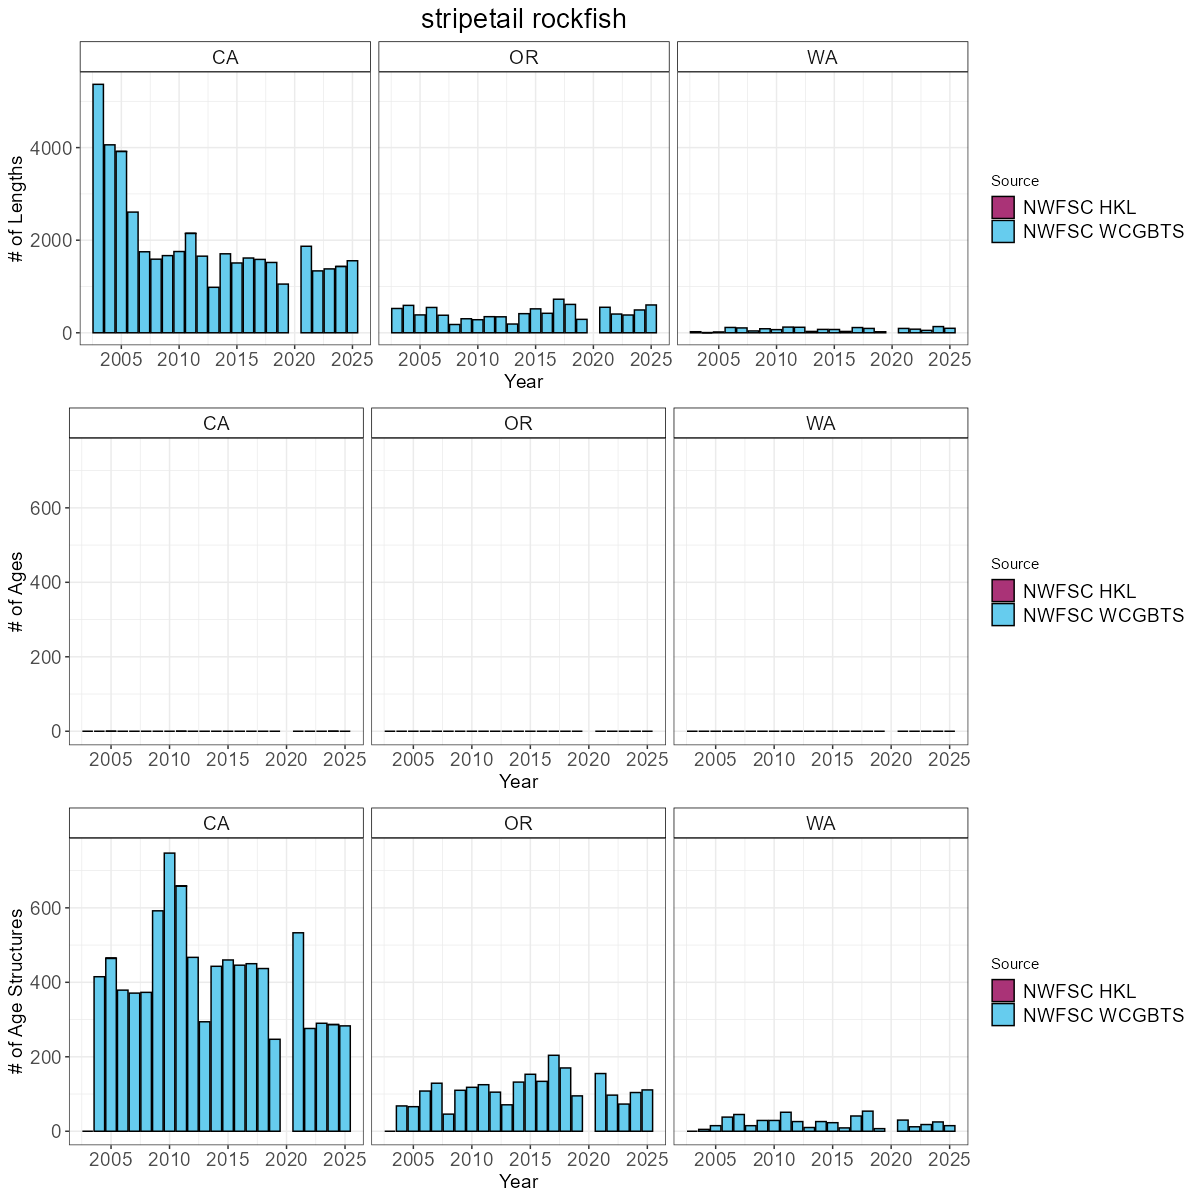
\includegraphics[keepaspectratio]{../plots/state_comparisons/stripetail_rockfish_state_compositions.png}}

}

\caption{Total number of available lengths, read ages, and unread age
structures by data source by year. Note the y-axis is unique for the
number of lengths plot row compared to the number of age and age
structure plot rows.}

\end{figure}%

\newpage{}

\subsection{Vermilion and sunset
rockfish}\label{vermilion-and-sunset-rockfish}

The most recent assessment of vermilion and sunset rockfish was a
benchmark assessment conducted in 2021. Across available data, vermilion
and sunset rockfish have been observed and sampled by both the NWFSC
WCGBT and HKL surveys. The NWFSC HKL survey has an average of 107
positive tows per year. The NWFSC WCGBTS survey has an average of 12
positive tows per year. Across the coast a total of 1728 maturity
samples have been collected with 1405 read maturities.

\begingroup\fontsize{10}{12}\selectfont
\begingroup\fontsize{10}{12}\selectfont

\begin{longtable}[t]{>{\raggedleft\arraybackslash}p{2cm}>{\raggedleft\arraybackslash}p{3.5cm}>{\raggedleft\arraybackslash}p{2cm}>{\raggedleft\arraybackslash}p{2cm}>{\raggedleft\arraybackslash}p{2cm}}
\caption{\label{tab:unnamed-chunk-202}Total number of available lengths, read ages, and unread age structures by data source and
state between for vermilion and sunset rockfish.}\\
\toprule
State & Source & Lengths & Ages & Age Structures\\
\midrule
\endfirsthead
\caption[]{Total number of available lengths, read ages, and unread age structures by data source and
state between for vermilion and sunset rockfish. (\textit{continued)}}\\
\toprule
State & Source & Lengths & Ages & Age Structures\\
\midrule
\endhead

\endfoot
\bottomrule
\endlastfoot
CA & NWFSC HKL & 42,075 & 15,460 & 16,189\\
CA & NWFSC WCGBTS & 3,432 & 1,753 & 717\\
OR & NWFSC WCGBTS & 2 & 2 & 0\\*
\end{longtable}
\endgroup{}
\endgroup{}

\begin{figure}[H]

{\centering \pandocbounded{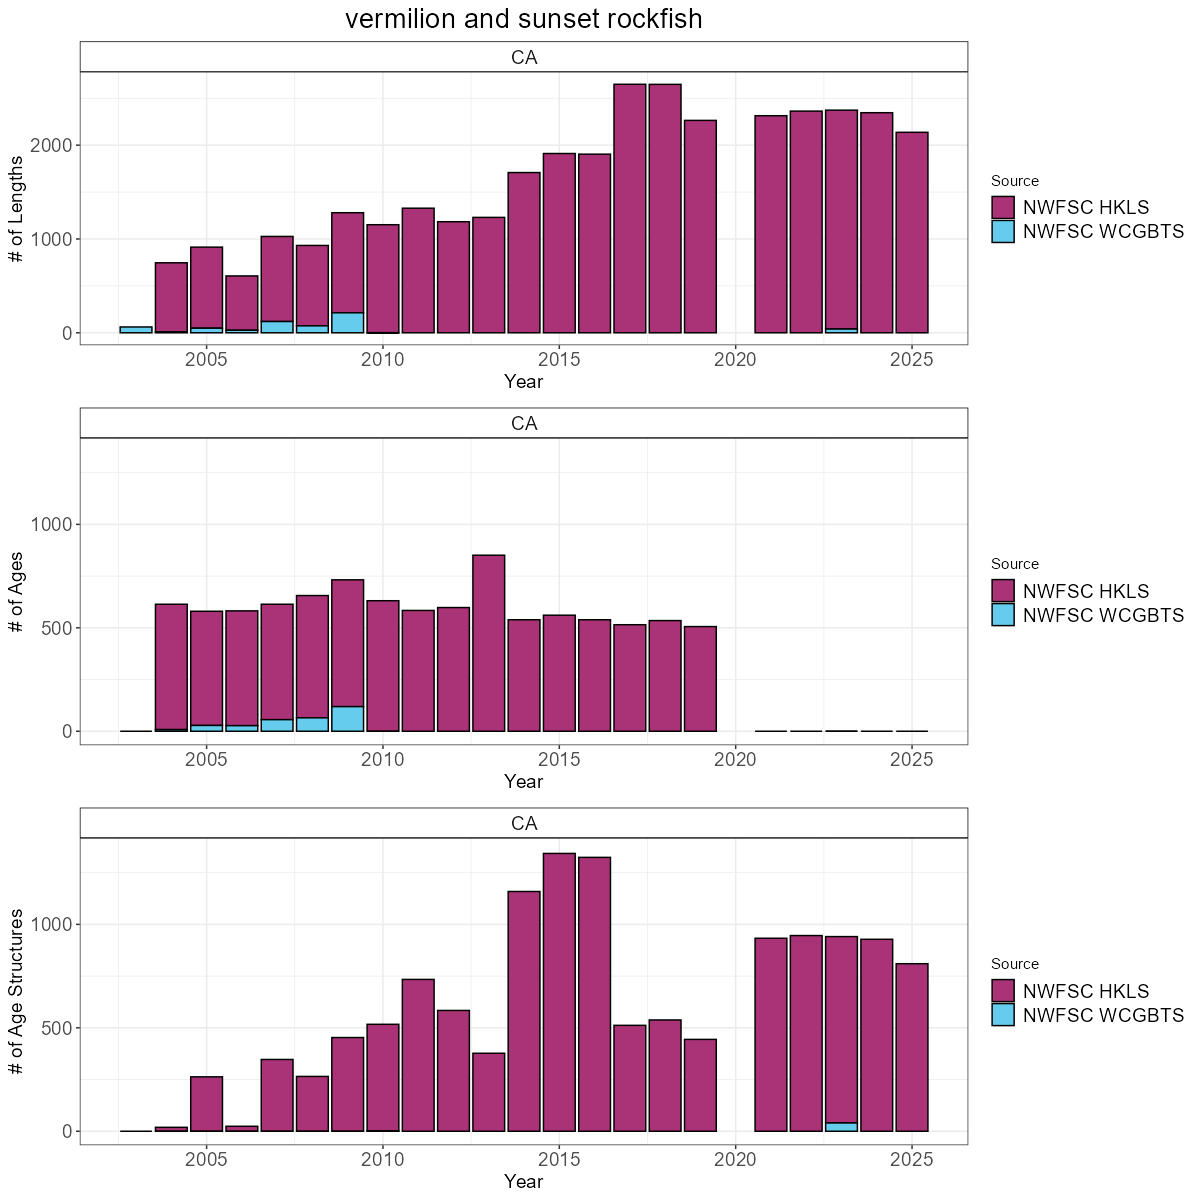
\includegraphics[keepaspectratio]{../plots/state_comparisons/vermilion_and_sunset_rockfish_state_compositions.png}}

}

\caption{Total number of available lengths, read ages, and unread age
structures by data source by year. Note the y-axis is unique for the
number of lengths plot row compared to the number of age and age
structure plot rows.}

\end{figure}%

\newpage{}

\subsection{Widow rockfish}\label{widow-rockfish}

The most recent assessment of widow rockfish was an update assessment
conducted in 2025. Across available data, widow rockfish have been
observed and sampled by both the NWFSC WCGBT and HKL surveys. The NWFSC
HKL survey has an average of 14 positive tows per year. The NWFSC WCGBTS
survey has an average of 24 positive tows per year. Across the coast a
total of 322 maturity samples have been collected with 92 read
maturities.

\begingroup\fontsize{10}{12}\selectfont
\begingroup\fontsize{10}{12}\selectfont

\begin{longtable}[t]{>{\raggedleft\arraybackslash}p{2cm}>{\raggedleft\arraybackslash}p{3.5cm}>{\raggedleft\arraybackslash}p{2cm}>{\raggedleft\arraybackslash}p{2cm}>{\raggedleft\arraybackslash}p{2cm}}
\caption{\label{tab:unnamed-chunk-207}Total number of available lengths, read ages, and unread age structures by data source and
state between for widow rockfish.}\\
\toprule
State & Source & Lengths & Ages & Age Structures\\
\midrule
\endfirsthead
\caption[]{Total number of available lengths, read ages, and unread age structures by data source and
state between for widow rockfish. (\textit{continued)}}\\
\toprule
State & Source & Lengths & Ages & Age Structures\\
\midrule
\endhead

\endfoot
\bottomrule
\endlastfoot
CA & NWFSC HKL & 899 & 0 & 877\\
CA & NWFSC WCGBTS & 1,985 & 1,363 & 9\\
OR & NWFSC WCGBTS & 2,161 & 1,417 & 10\\
WA & NWFSC WCGBTS & 921 & 520 & 4\\*
\end{longtable}
\endgroup{}
\endgroup{}

\begin{figure}[H]

{\centering \pandocbounded{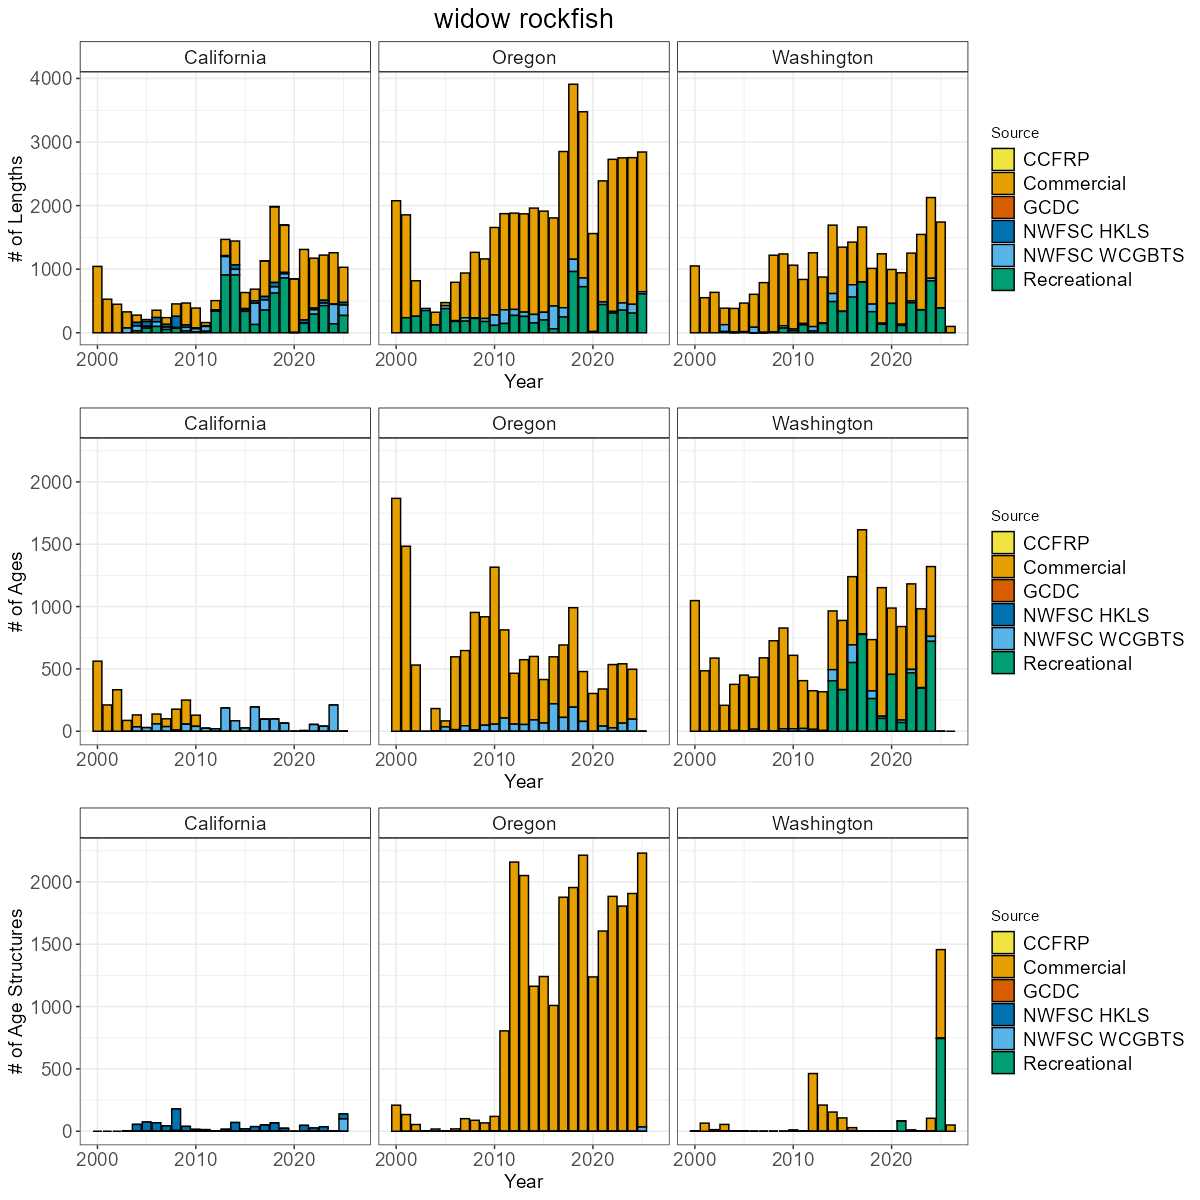
\includegraphics[keepaspectratio]{../plots/state_comparisons/widow_rockfish_state_compositions.png}}

}

\caption{Total number of available lengths, read ages, and unread age
structures by data source by year. Note the y-axis is unique for the
number of lengths plot row compared to the number of age and age
structure plot rows.}

\end{figure}%

\newpage{}

\subsection{Yelloweye rockfish}\label{yelloweye-rockfish}

The most recent assessment of yelloweye rockfish was an update
assessment conducted in 2025. Across available data, yelloweye rockfish
have been observed and sampled by both the NWFSC WCGBT and HKL surveys.
The NWFSC HKL survey has an average of 4 positive tows per year. The
NWFSC WCGBTS survey has an average of 15 positive tows per year. Across
the coast a total of 708 maturity samples have been collected with 119
read maturities.

\begingroup\fontsize{10}{12}\selectfont
\begingroup\fontsize{10}{12}\selectfont

\begin{longtable}[t]{>{\raggedleft\arraybackslash}p{2cm}>{\raggedleft\arraybackslash}p{3.5cm}>{\raggedleft\arraybackslash}p{2cm}>{\raggedleft\arraybackslash}p{2cm}>{\raggedleft\arraybackslash}p{2cm}}
\caption{\label{tab:unnamed-chunk-212}Total number of available lengths, read ages, and unread age structures by data source and
state between for yelloweye rockfish.}\\
\toprule
State & Source & Lengths & Ages & Age Structures\\
\midrule
\endfirsthead
\caption[]{Total number of available lengths, read ages, and unread age structures by data source and
state between for yelloweye rockfish. (\textit{continued)}}\\
\toprule
State & Source & Lengths & Ages & Age Structures\\
\midrule
\endhead

\endfoot
\bottomrule
\endlastfoot
CA & NWFSC HKL & 159 & 0 & 151\\
CA & NWFSC WCGBTS & 168 & 167 & 1\\
OR & NWFSC WCGBTS & 465 & 457 & 7\\
WA & NWFSC WCGBTS & 416 & 410 & 6\\*
\end{longtable}
\endgroup{}
\endgroup{}

\begin{figure}[H]

{\centering \pandocbounded{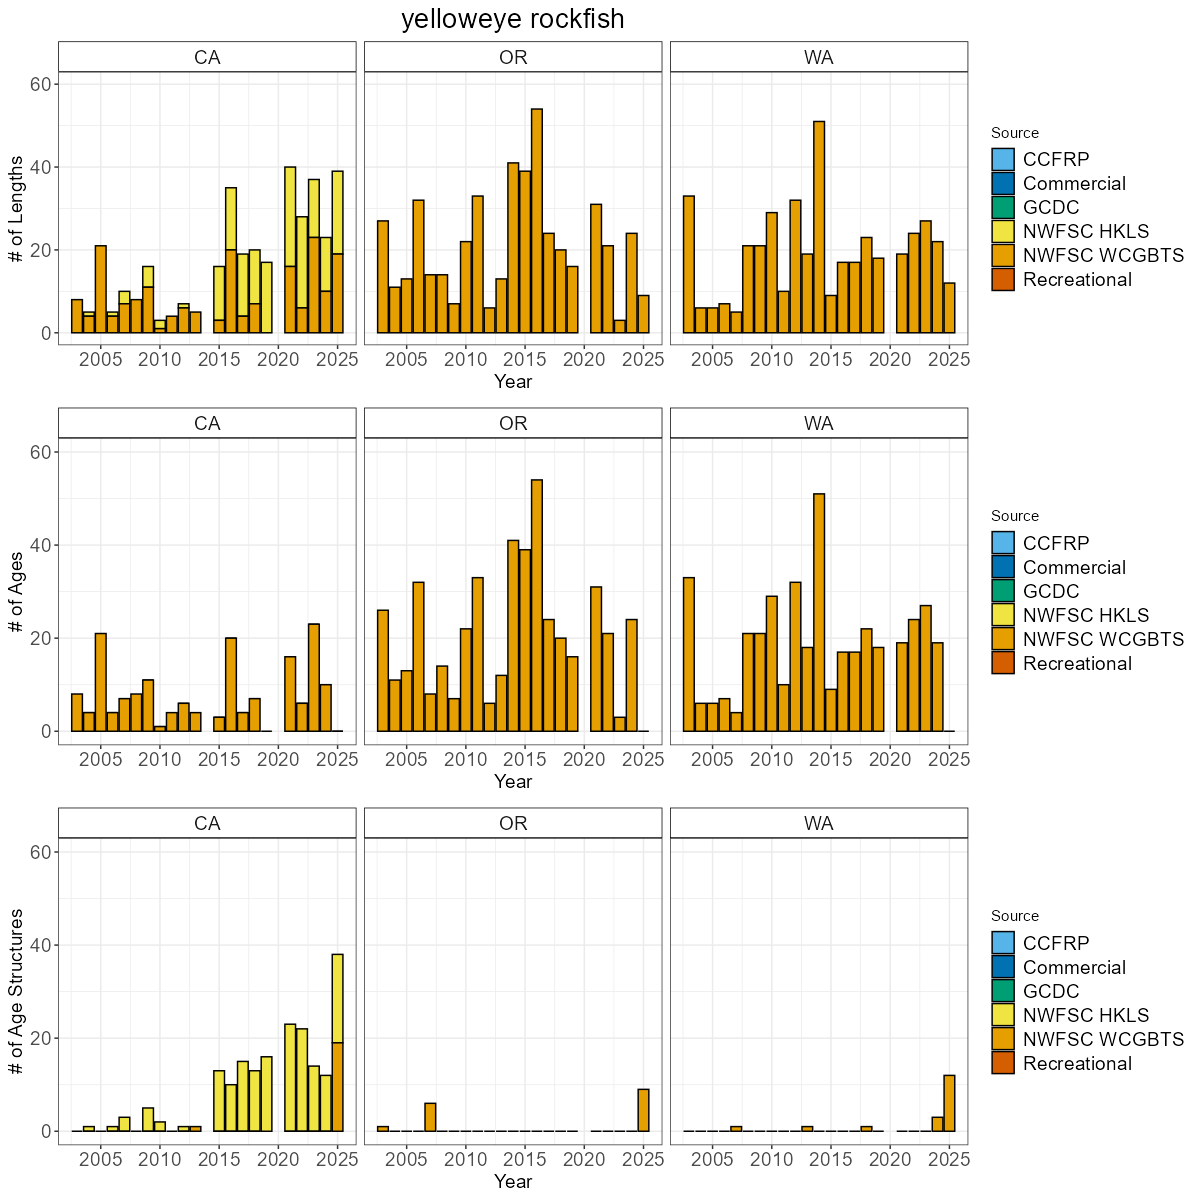
\includegraphics[keepaspectratio]{../plots/state_comparisons/yelloweye_rockfish_state_compositions.png}}

}

\caption{Total number of available lengths, read ages, and unread age
structures by data source by year. Note the y-axis is unique for the
number of lengths plot row compared to the number of age and age
structure plot rows.}

\end{figure}%

\newpage{}

\subsection{Yellowmouth rockfish}\label{yellowmouth-rockfish}

To date, no assessment or analysis has been conducted on yellowmouth
rockfish. Across available data, yellowmouth rockfish have been observed
and sampled by the NWFSC WCGBT survey. Across the coast a total of 12
maturity samples have been collected with 0 read maturities.

\begingroup\fontsize{10}{12}\selectfont
\begingroup\fontsize{10}{12}\selectfont

\begin{longtable}[t]{>{\raggedleft\arraybackslash}p{2cm}>{\raggedleft\arraybackslash}p{3.5cm}>{\raggedleft\arraybackslash}p{2cm}>{\raggedleft\arraybackslash}p{2cm}>{\raggedleft\arraybackslash}p{2cm}}
\caption{\label{tab:unnamed-chunk-217}Total number of available lengths, read ages, and unread age structures by data source and
state between for yellowmouth rockfish.}\\
\toprule
State & Source & Lengths & Ages & Age Structures\\
\midrule
\endfirsthead
\caption[]{Total number of available lengths, read ages, and unread age structures by data source and
state between for yellowmouth rockfish. (\textit{continued)}}\\
\toprule
State & Source & Lengths & Ages & Age Structures\\
\midrule
\endhead

\endfoot
\bottomrule
\endlastfoot
CA & NWFSC WCGBTS & 1 & 0 & 1\\
OR & NWFSC WCGBTS & 572 & 0 & 303\\
WA & NWFSC WCGBTS & 52 & 0 & 52\\*
\end{longtable}
\endgroup{}
\endgroup{}

\begin{figure}[H]

{\centering \pandocbounded{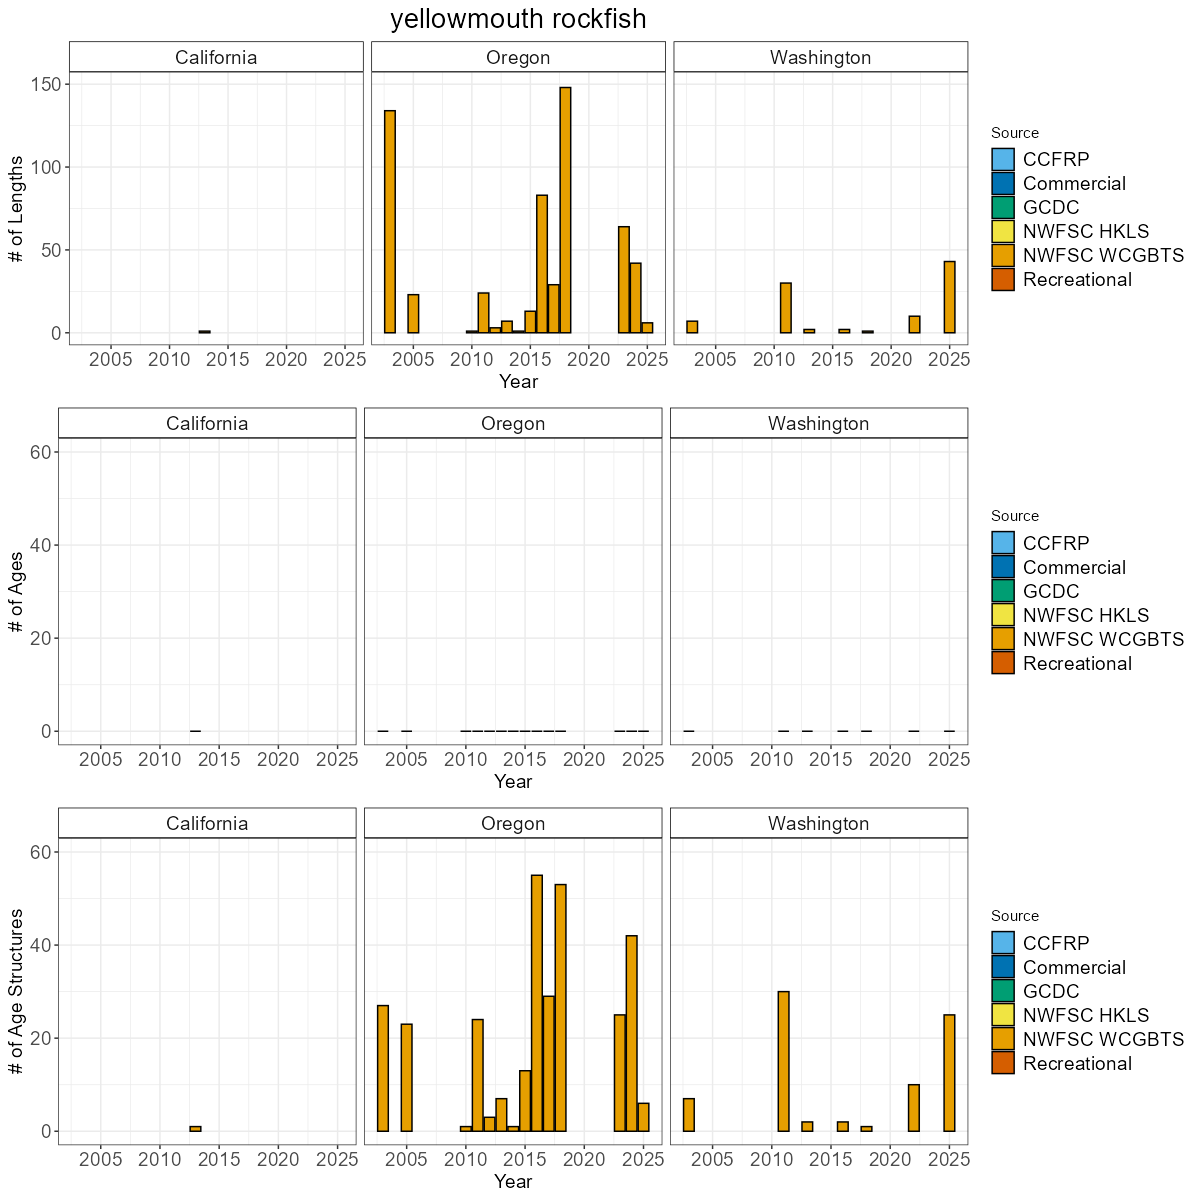
\includegraphics[keepaspectratio]{../plots/state_comparisons/yellowmouth_rockfish_state_compositions.png}}

}

\caption{Total number of available lengths, read ages, and unread age
structures by data source by year. Note the y-axis is unique for the
number of lengths plot row compared to the number of age and age
structure plot rows.}

\end{figure}%

\newpage{}

\subsection{Yellowtail rockfish north}\label{yellowtail-rockfish-north}

The most recent assessment of yellowtail rockfish north was a benchmark
assessment conducted in 2025. Across available data, yellowtail rockfish
north have been observed and sampled by the NWFSC WCGBT survey. The
NWFSC WCGBTS survey has an average of 41 positive tows per year. Across
the coast a total of 739 maturity samples have been collected with 672
read maturities. ODFW scientists are planning a research cruise to Cobb
Sea Mount in the summer of 2026 to sample age and sex distributions of
rockfish species.

\begingroup\fontsize{10}{12}\selectfont
\begingroup\fontsize{10}{12}\selectfont

\begin{longtable}[t]{>{\raggedleft\arraybackslash}p{2cm}>{\raggedleft\arraybackslash}p{3.5cm}>{\raggedleft\arraybackslash}p{2cm}>{\raggedleft\arraybackslash}p{2cm}>{\raggedleft\arraybackslash}p{2cm}}
\caption{\label{tab:unnamed-chunk-222}Total number of available lengths, read ages, and unread age structures by data source and
state between for yellowtail rockfish north.}\\
\toprule
State & Source & Lengths & Ages & Age Structures\\
\midrule
\endfirsthead
\caption[]{Total number of available lengths, read ages, and unread age structures by data source and
state between for yellowtail rockfish north. (\textit{continued)}}\\
\toprule
State & Source & Lengths & Ages & Age Structures\\
\midrule
\endhead

\endfoot
\bottomrule
\endlastfoot
CA & NWFSC WCGBTS & 792 & 292 & 27\\
OR & NWFSC WCGBTS & 3,912 & 1,947 & 404\\
WA & NWFSC WCGBTS & 12,624 & 5,633 & 877\\*
\end{longtable}
\endgroup{}
\endgroup{}

\begin{figure}[H]

{\centering \pandocbounded{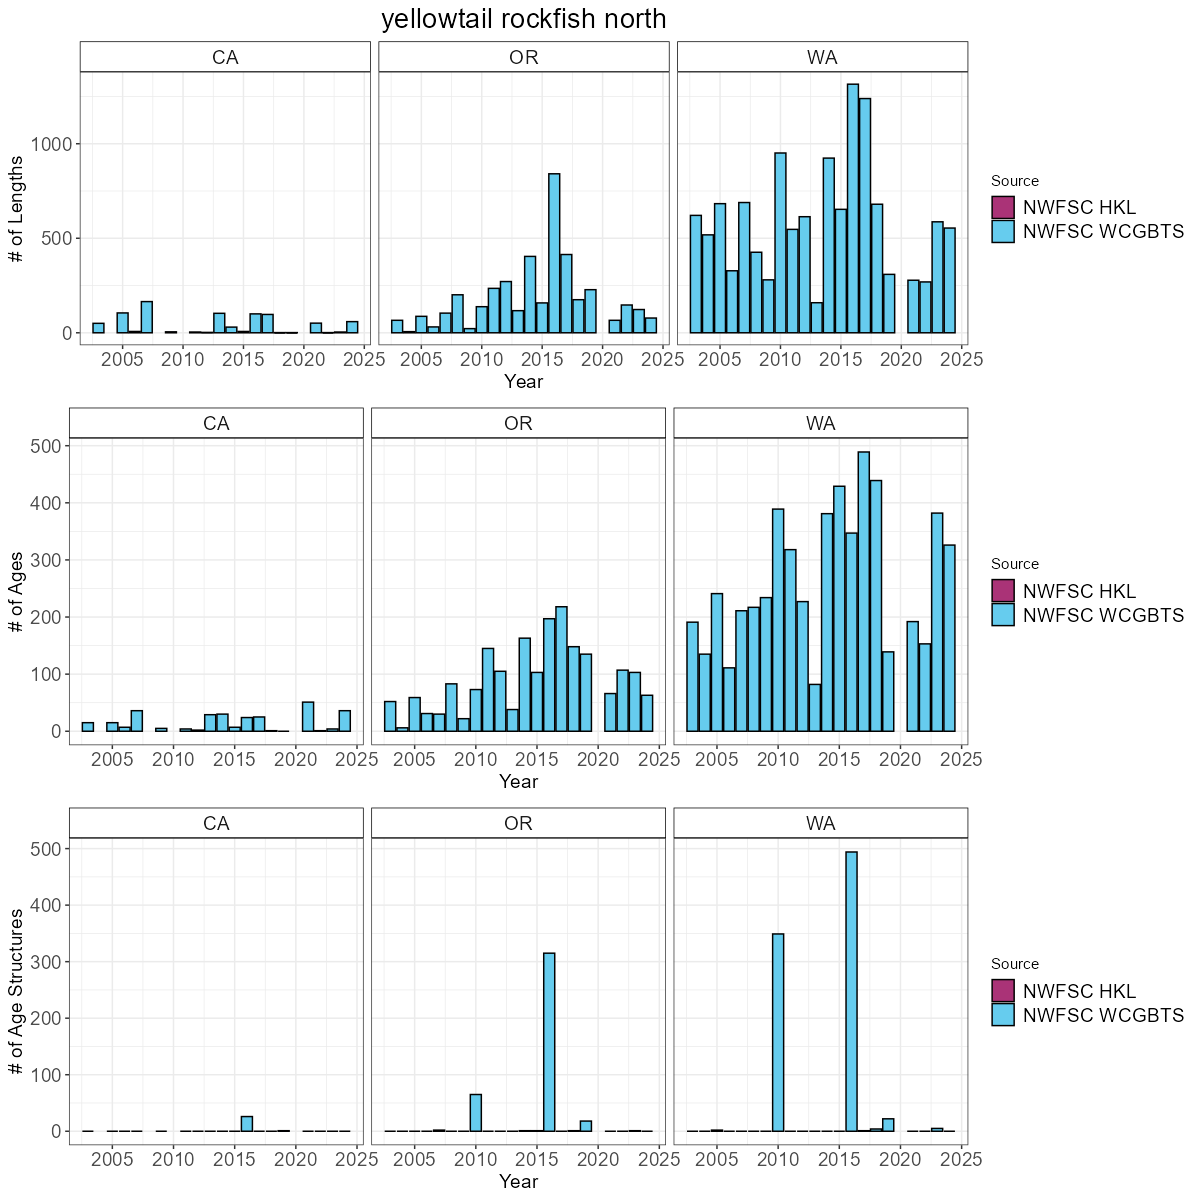
\includegraphics[keepaspectratio]{../plots/state_comparisons/yellowtail_rockfish_north_state_compositions.png}}

}

\caption{Total number of available lengths, read ages, and unread age
structures by data source by year. Note the y-axis is unique for the
number of lengths plot row compared to the number of age and age
structure plot rows.}

\end{figure}%

\newpage{}

\subsection{Yellowtail rockfish south}\label{yellowtail-rockfish-south}

To date, no assessment or analysis has been conducted on yellowtail
rockfish south. Across available data, yellowtail rockfish south have
been observed and sampled by both the NWFSC WCGBT and HKL surveys. The
NWFSC HKL survey has an average of 13 positive tows per year. Across the
coast a total of 739 maturity samples have been collected with 672 read
maturities.

\begingroup\fontsize{10}{12}\selectfont
\begingroup\fontsize{10}{12}\selectfont

\begin{longtable}[t]{>{\raggedleft\arraybackslash}p{2cm}>{\raggedleft\arraybackslash}p{3.5cm}>{\raggedleft\arraybackslash}p{2cm}>{\raggedleft\arraybackslash}p{2cm}>{\raggedleft\arraybackslash}p{2cm}}
\caption{\label{tab:unnamed-chunk-227}Total number of available lengths, read ages, and unread age structures by data source and
state between for yellowtail rockfish south.}\\
\toprule
State & Source & Lengths & Ages & Age Structures\\
\midrule
\endfirsthead
\caption[]{Total number of available lengths, read ages, and unread age structures by data source and
state between for yellowtail rockfish south. (\textit{continued)}}\\
\toprule
State & Source & Lengths & Ages & Age Structures\\
\midrule
\endhead

\endfoot
\bottomrule
\endlastfoot
CA & NWFSC HKL & 1,907 & 124 & 1,564\\
CA & NWFSC WCGBTS & 1,072 & 534 & 21\\*
\end{longtable}
\endgroup{}
\endgroup{}

\begin{figure}[H]

{\centering \pandocbounded{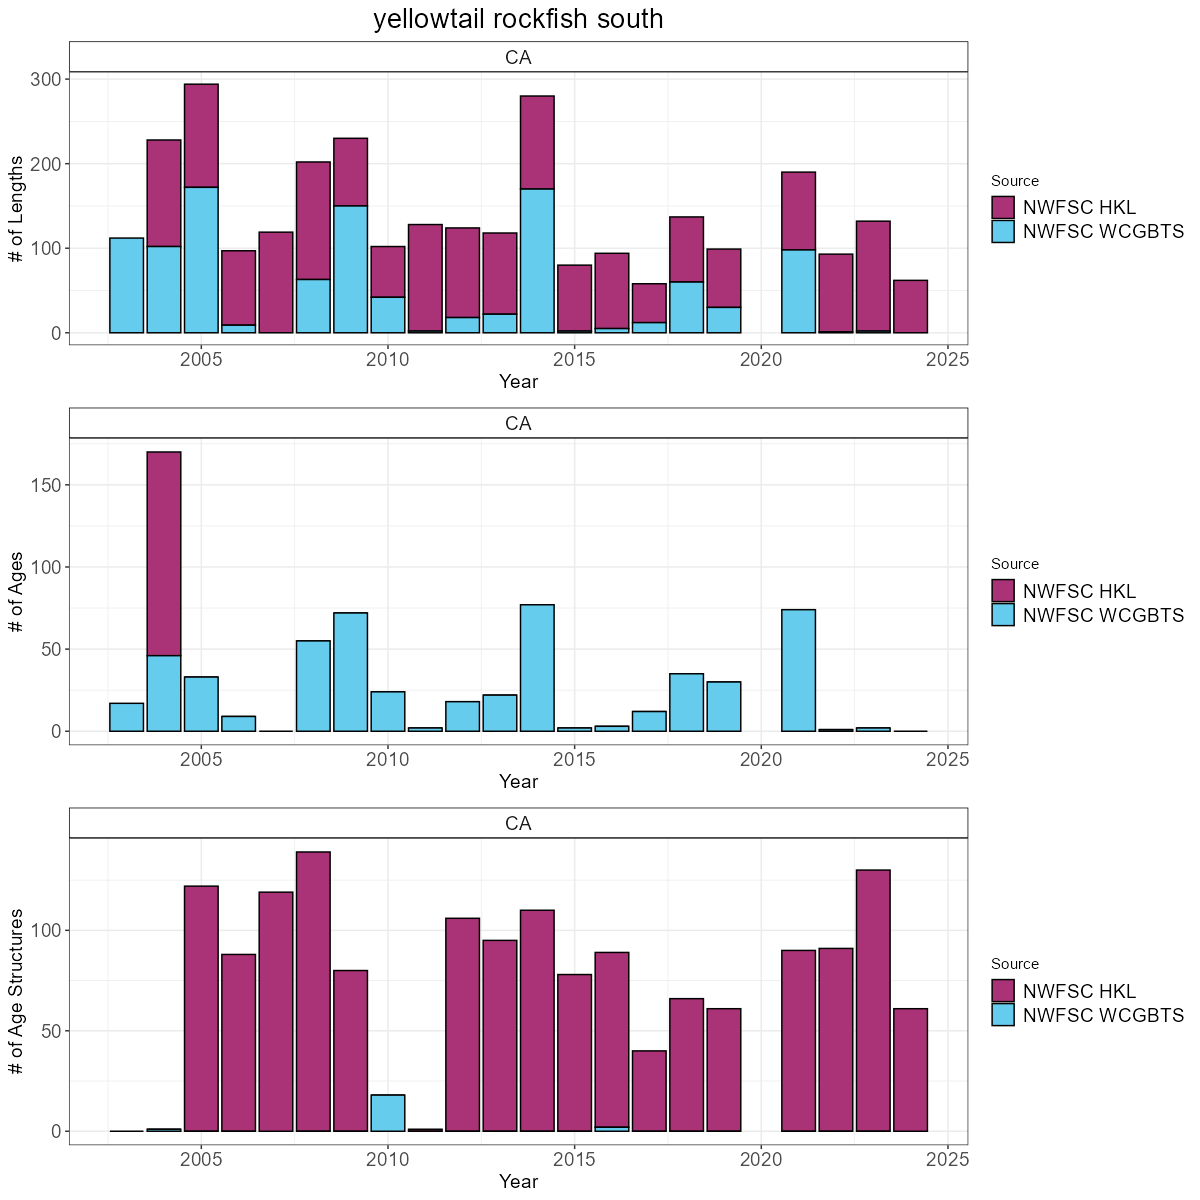
\includegraphics[keepaspectratio]{../plots/state_comparisons/yellowtail_rockfish_south_state_compositions.png}}

}

\caption{Total number of available lengths, read ages, and unread age
structures by data source by year. Note the y-axis is unique for the
number of lengths plot row compared to the number of age and age
structure plot rows.}

\end{figure}%

\newpage{}

\section{Index Estimation for the NWFSC WCGBT
Survey}\label{wcgbt-index-settings}

\begingroup\fontsize{7}{9}\selectfont

\begin{landscape}\begingroup\fontsize{7}{9}\selectfont

\begin{longtable}[t]{>{\raggedright\arraybackslash}p{0.1 cm}>{\raggedright\arraybackslash}p{2.5 cm}>{\raggedright\arraybackslash}p{2.5 cm}>{\raggedright\arraybackslash}p{4 cm}>{\raggedright\arraybackslash}p{1 cm}>{\raggedright\arraybackslash}p{1 cm}>{\raggedright\arraybackslash}p{1 cm}>{\raggedright\arraybackslash}p{0.1 cm}>{\raggedright\arraybackslash}p{2.5 cm}>{\raggedright\arraybackslash}p{2.5 cm}>{\raggedright\arraybackslash}p{4 cm}>{\raggedright\arraybackslash}p{1 cm}>{\raggedright\arraybackslash}p{1 cm}>{\raggedright\arraybackslash}p{1 cm}>{\raggedright\arraybackslash}p{0.1 cm}>{\raggedright\arraybackslash}p{2.5 cm}>{\raggedright\arraybackslash}p{2.5 cm}}
\caption{\label{tab:survey-settings}Setting used for estimating indices of abundance for the NWFSC WCGBT survey by species.}\\
\toprule
species & family & formula & min latitude & max latitude & spatiotemporal1 & spatiotemporal2\\
\midrule
\endfirsthead
\caption[]{Setting used for estimating indices of abundance for the NWFSC WCGBT survey by species. (\textit{continued)}}\\
\toprule
species & family & formula & min latitude & max latitude & spatiotemporal1 & spatiotemporal2\\
\midrule
\endhead

\endfoot
\bottomrule
\endlastfoot
canary rockfish & delta\_lognormal() & catch\_weight \textasciitilde{} 0 + fyear + pass\_scaled & 31.9 & 49.0 & iid & off\\
chilipepper & delta\_lognormal() & catch\_weight \textasciitilde{} 0 + fyear + pass\_scaled + depth\_scaled + depth\_scaled\_squared & 31.9 & 46.2 & iid & off\\
rougheye rockfish & delta\_lognormal() & catch\_weight \textasciitilde{} 0 + fyear + pass\_scaled & 42.0 & 49.0 & off & off\\
sablefish & delta\_gamma() & catch\_weight \textasciitilde{} 0 + fyear + pass\_scaled & 31.9 & 49.0 & iid & iid\\
widow rockfish & delta\_lognormal() & catch\_weight \textasciitilde{} 0 + fyear + pass\_scaled & 33.5 & 49.0 & iid & off\\
yelloweye rockfish & delta\_lognormal() & catch\_weight \textasciitilde{} 0 + fyear + pass\_scaled & 42.0 & 49.0 & off & off\\
yellowtail rockfish & delta\_lognormal() & catch\_weight \textasciitilde{} 0 + fyear*split\_mendocino + pass\_scaled & 33.5 & 49.0 & iid & off\\*
\end{longtable}
\endgroup{}
\end{landscape}
\endgroup{}

\newpage

\section{Acknowledgement}\label{acknowledgement}

We would like to thank the NWFSC Fisheries Resource Analysis and
Monitoring survey team and their dedication to collecting high quality
data that are essential to the assessment of West Coast groundfish
stocks.




\end{document}
